% Reconstruction in LArTPC
% Target length: 30 pages

\graphicspath{{LArTPCReconstruction/Figs/}}

%----------------------------------------------------------------------------------------------------------------------------------------------------------------------------
\chapter{Reconstruction in a Liquid Argon TPC}\label{chap:LArTPCReconstruction}

{\color{red} Should the title of this chapter reflect more of the original work which is discussed within?  e.g. Shower Reconstruction in a Liquid Argon TPC?  Although  it is a general reconstruction chapter, everything in Shower Reconstruction in LArTPCs is original.}

The use of LArTPCs in future high-precision projects, such as long-baseline neutrino experiments, is very well motivated by the unprecedented spatial and energy resolution available to detectors utilising the technology.  In order to take advantage of all this accessible information, accurate reconstruction must be developed to perform pattern recognition and energy determination for use by the proceeding analyses.  The techniques and status of reconstruction in LArTPCs is the subject of this chapter, with particular focus on novel methods developed for the reconstruction of electromagnetic showers.

The implementation of the reconstruction algorithms discussed in this chapter utilises the Liquid Argon Software framework (LArSoft), developed at FNAL and shared between all experiments in the LAr program.  LArSoft will be overviewed in Section~\ref{sec:LArSoft} before the reconstruction chain is described in Section~\ref{sec:ReconstructionChain}.  The development of new techniques in the reconstruction of showers will compose the main discussion in this chapter and is contained in Section~\ref{sec:ShowerReconstruction}.

%----------------------------------------------------------------------------------------------------------------------------------------------------------------------------
\section{The LArSoft Framework}\label{sec:LArSoft}

The Liquid Argon Software (LArSoft) \cite{LArSoftWebsite,LArSoft2013,LArSoft2016,Snider2016} collaboration supports the development, use, sharing and distributing of code utilised by all LAr experiments at FNAL.  The LArSoft framework is written in C++ and built on \textit{art} \cite{artWebsite,art2012}, the event-processing system established at FNAL and used by offline code developed for most experiments hosted at the lab.  As data from most LArTPC experiments share a similar basic format, LArSoft is envisioned to be agnostic to the detector specifics and provide a common interface, infrastructure and algorithms for simulation, reconstruction and analysis.  Along with vastly reducing duplicated effort, this also allows access to the most advanced software developments for smaller collaborations who otherwise may not have the required resources.

LArSoft provides well defined interfaces to various external packages, such as GENIE \cite{GENIE2010} and GEANT4 \cite{GEANT42006}, and access by particular experiments utilises configurable descriptions of the detector geometry, the electronics, detector response and other unique features.  This structure is demonstrated in Figure~\ref{fig:LArSoftStructure}.  This architecture ensures a flexible structure which facilitates the addition and evolution of algorithms and with contingency for future developments to be introduced with ease.

\begin{figure}
  \centering
  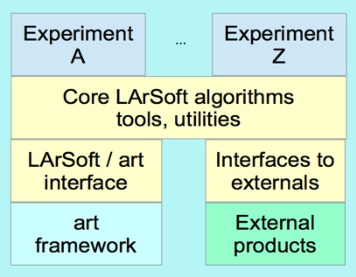
\includegraphics[width=7cm]{LArSoftStructure.pdf}
  \caption[The LArSoft architecture, highlighting support for both common and experiment-specific algorithms and methods and the interfacing with other packages.]{The LArSoft architecture, highlighting support for both common and experiment-specific algorithms and methods and the interfacing with other packages.  Taken from \cite{LArSoft2016}.}
  \label{fig:LArSoftStructure}
\end{figure}

The \textit{art} framework provides an interface to the information stored for each event by user-written `modules' and handles execution by processing each entry and making the data available to these plug-in modules.  Additionally, `services', which exist outside of the event structure, are provided and may be used to obtain general information such as detector geometry or LAr properties whenever needed.  The two main module types, named \texttt{Analyzers} (sic) and \texttt{Producers}, can access the data products stored in a particular event and, in the case of \texttt{Producers}, have the ability to place data into the event for use in future processes.  All modules, regardless of their type, have only read-only access to the existing information in the event.  Configuration of an \textit{art} job utilises the custom Fermilab Hierarchical Configuration Language (\textit{fhicl}, pronounced `fickle') which may be used to define the modules (including their order) and services to be run and to provide run-time parameters for use by these products.

The end-to-end configuration for a given experiment involves the following standard stages: generation (provided by a generator, such as GENIE), propagation (executed with GEANT4), detector response simulation, and reconstruction.  The results from the first three steps aim to reproduce as closely as possible the expectations from real data, with the same reconstruction applied to both the simulated output from the detector and data.  The processes are configured, using \texttt{Producer} modules, in \textit{art} using \textit{fhicl}, generally separated into four jobs representing each of the stages.

LArSoft was initially developed for use in ArgoNeuT in around 2011 and has since progressed into the large collaboration which it is today, with more than 100 code authors spanning multiple experiments.  The constant progression of algorithms have resulted in very well-developed, advanced simulation and reconstruction tools with corresponding shared expertise.  The recent uses of LArSoft reconstruction on real data, in MicroBooNE \cite{MicroBooNEReconstruction2017} and the 35~ton (Chapter~\ref{chap:35tonAnalysis}), are providing an excellent test of the efficacy of the simulation along with the validation of reconstruction applied to data.  The current reconstruction chain is discussed in Section~\ref{sec:ReconstructionChain}.

Until recently, convincing electromagnetic shower reconstruction has not existed within LArSoft.  Despite this being a major advantage of LArTPCs, it is particularly challenging and requires significant investment of resources to fully understand.  This motivated the development of new algorithms within the LArSoft framework, BlurredCluster and EMShower, which will be discussed in detail in Section~\ref{sec:ShowerReconstruction}.

%----------------------------------------------------------------------------------------------------------------------------------------------------------------------------
\section{The Reconstruction Chain}\label{sec:ReconstructionChain}

Reconstruction in LArSoft is the process of forming particle objects, with enough information to be able to perform identification, from the raw charge read out by the anode planes.  The process may be considered as three main components: calibrating the raw charge to remove detector effects; pattern recognition; calorimetry.  These will be discussed in Sections~\ref{sec:HitReconstruction},~\ref{sec:PatternRecognition} and~\ref{sec:Calorimetry} respectively.  The general workflow is shown schematically in Figure~\ref{fig:ReconstructionWorkflow}.

\begin{figure}
  \centering
  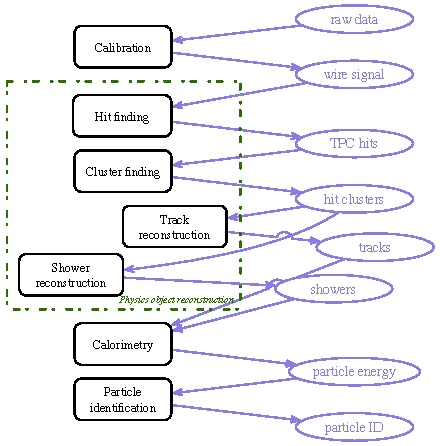
\includegraphics[width=8cm]{ReconstructionWorkflow.pdf}
  \caption[The LArSoft reconstruction workflow to produce 3D reconstructed objects from the raw charge read out by the anode wires.]{The LArSoft reconstruction workflow to produce 3D reconstructed objects from the raw charge read out by the anode wires \cite{LArSoft2016}.  The status of the reconstruction is shown on the right, with the various algorithms and their outputs represented on the left.}
  \label{fig:ReconstructionWorkflow}
\end{figure}

%----------------------------------------------------------------------------------------------------------------------------------------------------------------------------
\subsection{Raw Charge Calibration}\label{sec:HitReconstruction}

The charge induced and collected on the readout wires is modified by detector effects which must be well understood in order to be properly accounted for.  The measured waveform, $p(t)$, obtained from the signal $s(t)$, measured as a function of time $t$, can be represented in pseudocode as
\begin{equation}
  p(t) = \left( s(t) \otimes e(t) \otimes f(t) \right) + n(t),
\end{equation}
where $e$ is the electronics response, $f$ is the field response and $n$ is the noise in the detector.  Together, $e(t) \otimes f(t)$ are referred to as the detector response.

The first step in the reconstruction, referred to as the `deconvolution stage', involves removing these detector responses.  This proceeds by subtracting the noise profile from the measured waveform before Fourier transforming into frequency space and dividing out the field and electronics components.  The detector responses must be accurate and the models used have been developed at test stands to ensure they best represent the detector effects.  This process is applied in reverse during the detector simulation stage of the simulation to reproduce the expectations from the data as much as possible.

The detector response is demonstrated in Figure~\ref{fig:DetectorResponse}.  The principle of current induction on the anode wires is described by the Shockley-Ramo \cite{Shockley1938,Ramo1939} theorem; the instantaneous induced current $i$ is given by
\begin{equation}
  i = q \vec{E_w} \cdot \vec{v_q},
\end{equation}
where $q$ is the charge of an element of ionisation, $\vec{E_w}$ is the field vector at the location of the charge and $\vec{v_q}$ is the velocity of the charge packet \cite{MicroBooNERawCharge2016}.  The electric potential for the full wire planes is based on a 2D Garfield simulation \cite{GarfieldWebsite}; simulated TPC signals for each of the planes are demonstrated in Figure~\ref{fig:FieldResponse}.  The induced current is received, amplified and shaped by the preamplifier in the front end electronics.  Typical shaping times and gains are demonstrated in Figure~\ref{fig:ElectronicsResponse}.

\begin{figure}
  \centering
  \begin{subfigure}[t]{0.48\linewidth}
    \centering
    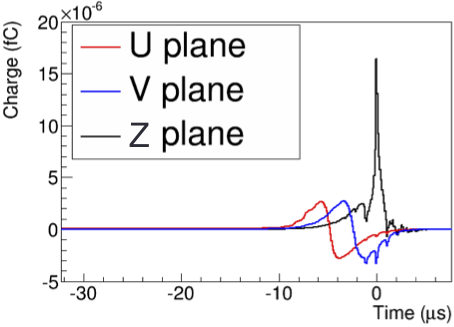
\includegraphics[width=0.98\textwidth]{FieldResponse.png}
    \caption{Field response.}
    \label{fig:FieldResponse}
  \end{subfigure}
  \hfill
  \begin{subfigure}[t]{0.48\linewidth}
    \centering
    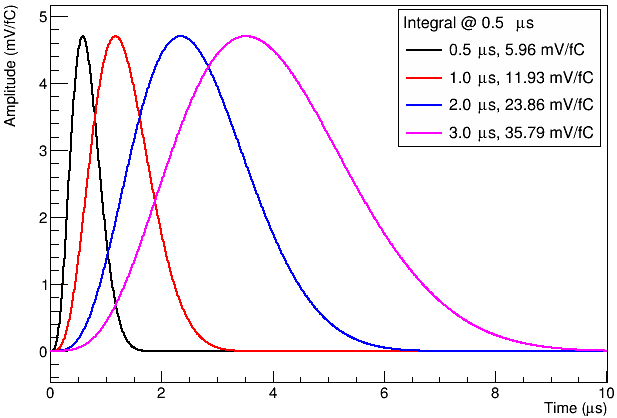
\includegraphics[width=0.98\textwidth]{ElectronicsResponse.png}
    \caption{Electronics response.}
    \label{fig:ElectronicsResponse}
  \end{subfigure}
  \caption[Detector response for charge readout in a LArTPC.]{Detector response for charge readout in a LArTPC.  The field response is shown in Figure~\ref{fig:FieldResponse} and the electronics response, set as configurable front end electronics settings, is demonstrated in Figure~\ref{fig:ElectronicsResponse}.  Based on descriptions in \cite{MicroBooNERawCharge2016}.}
  \label{fig:DetectorResponse}
\end{figure}

Following the deconvolution stage, the waveforms all have the form of a unipolar pulse.  The reconstruction proceeds with `hit finding', with the purpose to accurately determine the properties of the collected charge.  In particular, the peak time, width and total charge of the `hit's are pertinent for future reconstruction algorithms.  This is typically achieved by fitting a Gaussian to the pulse and using this to aid the determination of the hit properties.  The result of the deconvolution and hit finding stages are represented for simulated hits on three separate planes in Figure~\ref{fig:HitFinding}.  The hit finder used here is the Gaussian Hit Finder in LArSoft.

\begin{figure}
  \centering
  \begin{subfigure}[t]{0.3\linewidth}
    \centering
    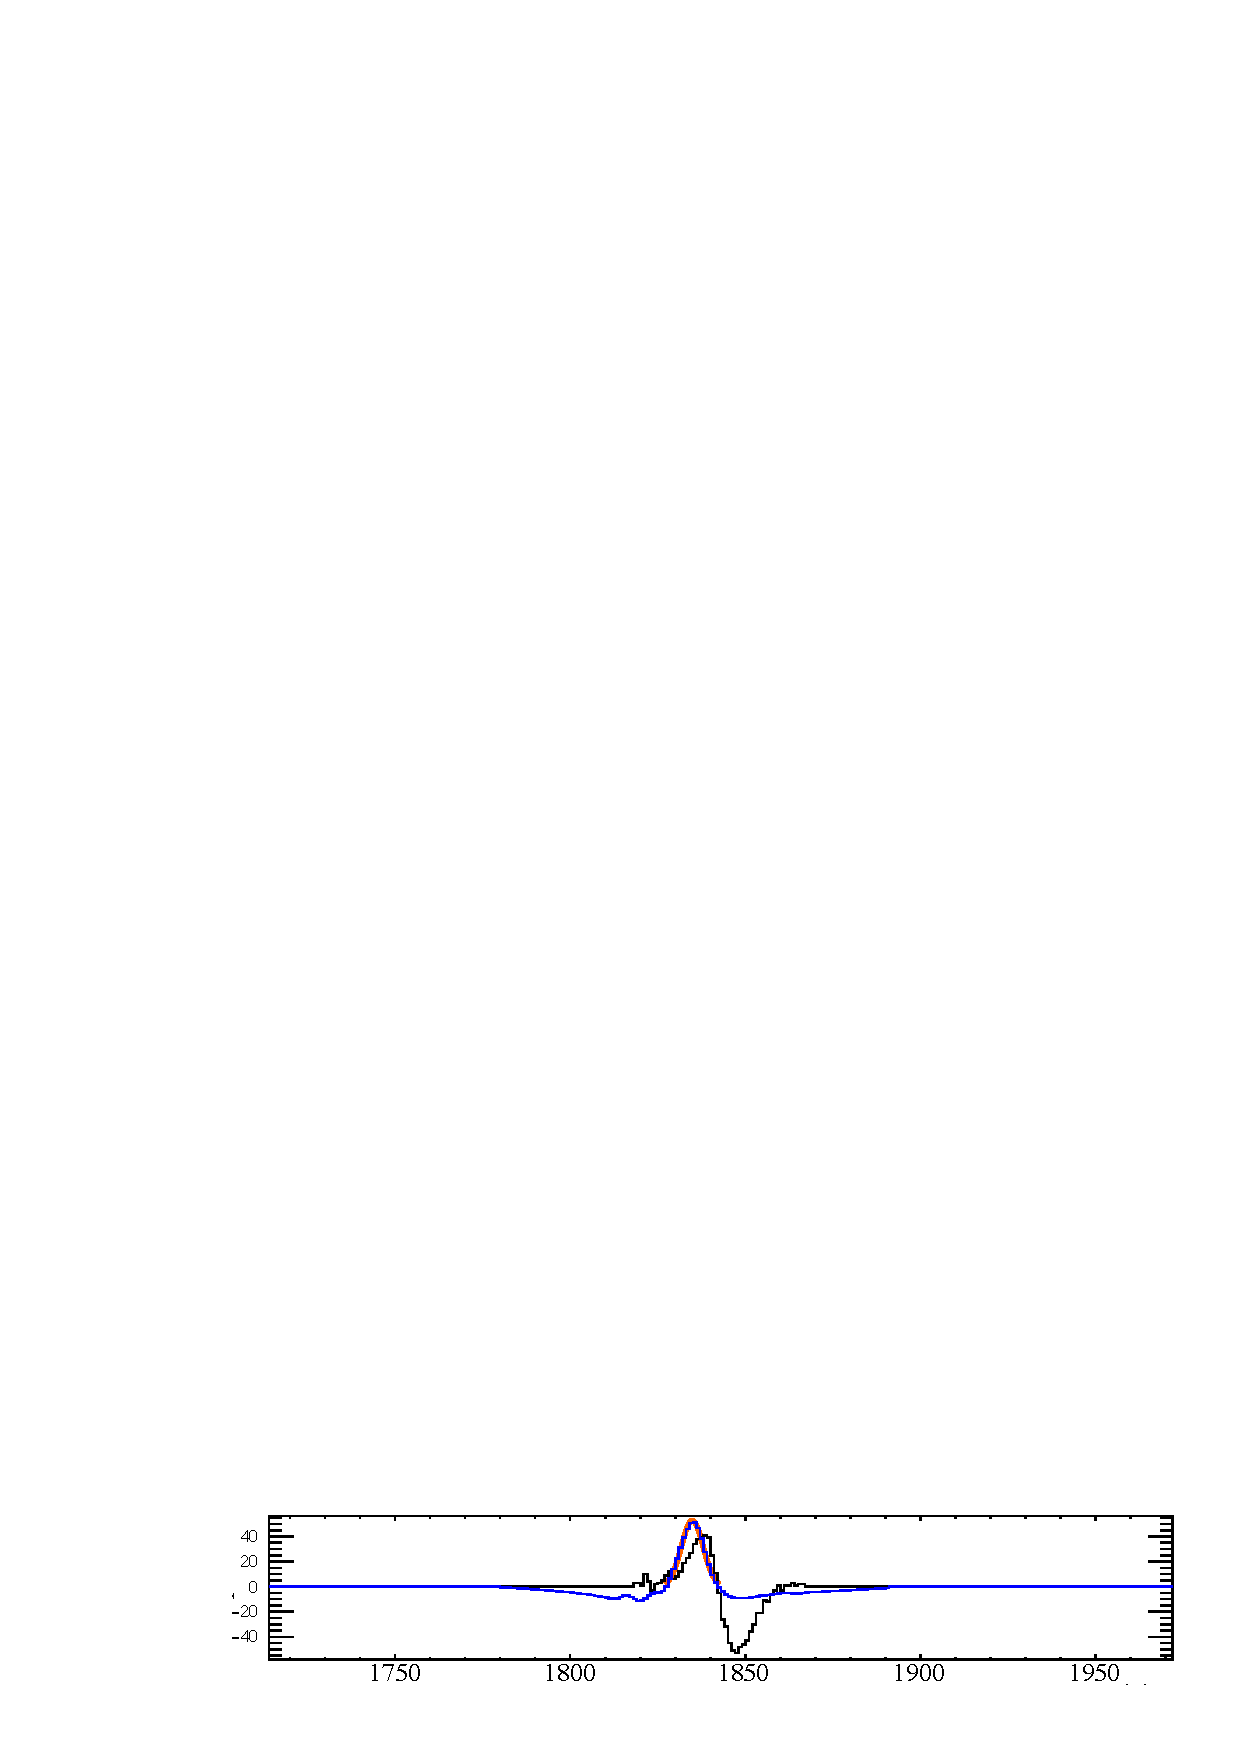
\includegraphics[width=\textwidth]{HitFindingU.pdf}
    \caption{U plane.}
    \label{fig:HitFindingU}
  \end{subfigure}
  \hfill
  \begin{subfigure}[t]{0.3\linewidth}
    \centering
    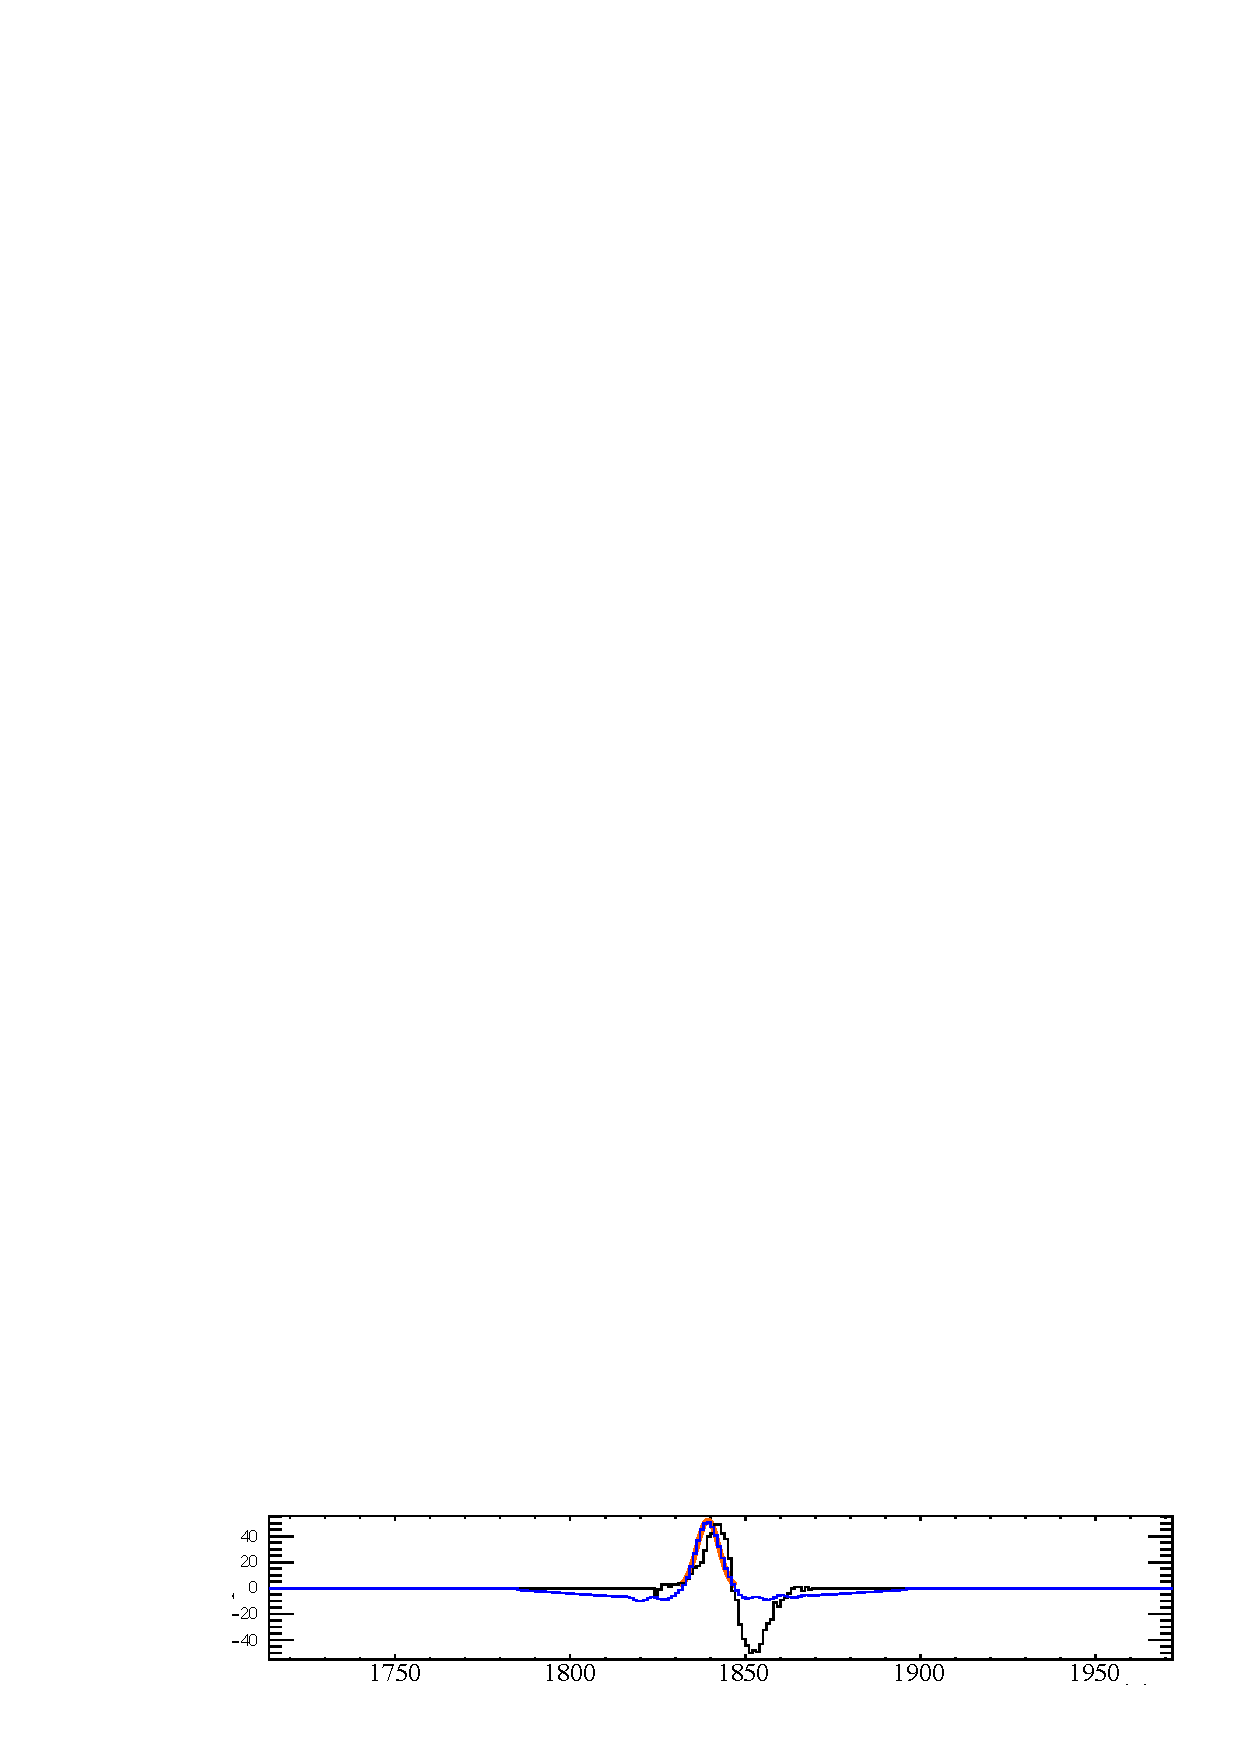
\includegraphics[width=\textwidth]{HitFindingV.pdf}
    \caption{V plane.}
    \label{fig:HitFindingV}
  \end{subfigure}
  \hfill
  \begin{subfigure}[t]{0.3\linewidth}
    \centering
    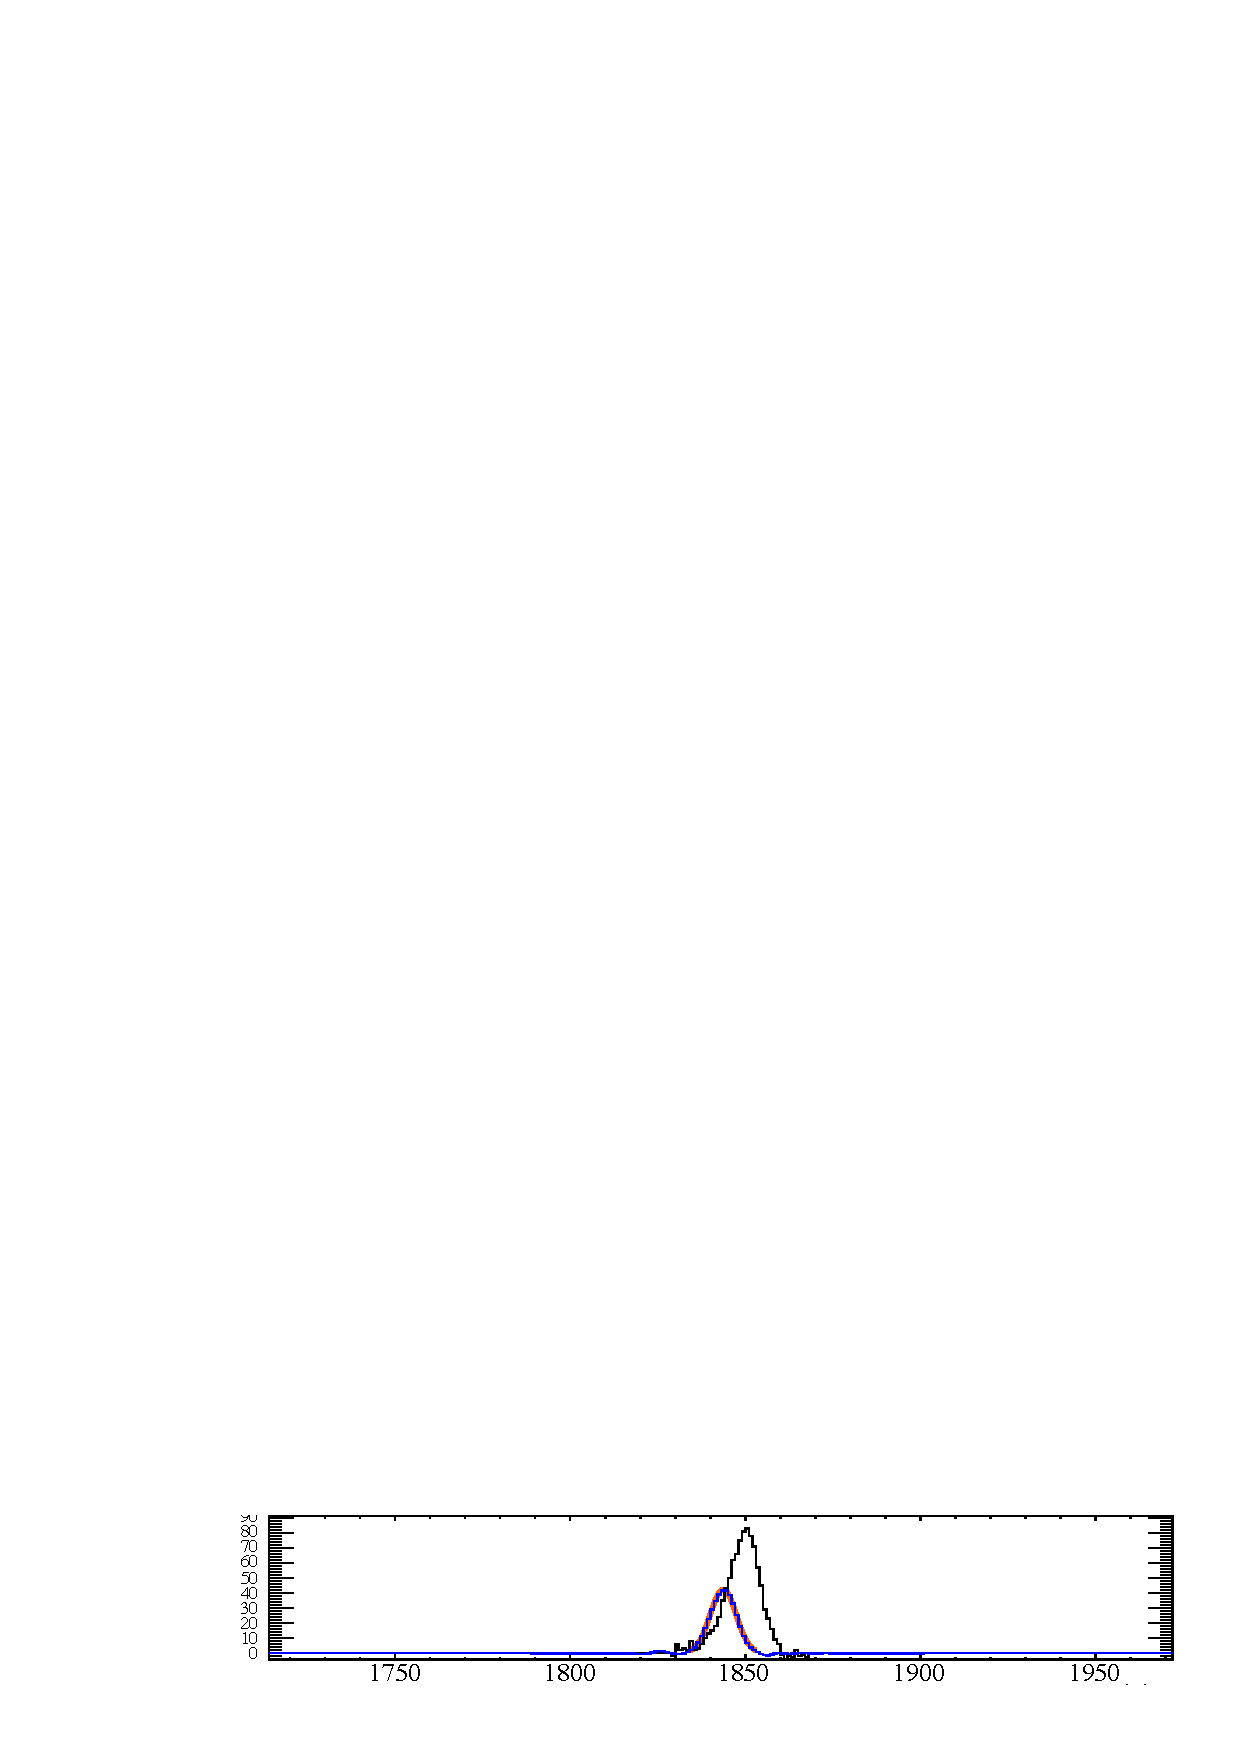
\includegraphics[width=\textwidth]{HitFindingZ.pdf}
    \caption{Z plane.}
    \label{fig:HitFindingZ}
  \end{subfigure}
  \caption[The process of deconvolution and hit finding to determine the correct charge from the measured pulses on the readout wires.]{The process of deconvolution and hit finding to determine the correct charge from the measured pulses on the readout wires.  Each 2D plane is represented as charge (ADC) as a function of time (tick).  In each case, the black waveform represents the raw measurement, the blue shows the outcome of deconvolution and the pink peak indicates the reconstructed hit.  Note the normalisation of the deconvoluted signal has been fixed to provide a factor four amplification for illustratory purposes.  The shift in time and shape is a result of the deconvolution from the electronics response (demonstrated in Figure~\ref{fig:ElectronicsResponse}).}
  \label{fig:HitFinding}
\end{figure}

Due to the wrapped wires, multiple hits will be reconstructed on each channel, one for each possible wire segment.  The final stage of hit processing is to perform disambiguation to select the correct hit for use in subsequent algorithms.  As previously discussed (Section~\ref{sec:DUNESinglePhase} and Section~\ref{sec:35tonTPC}), this is trivial in the far detector design as the wire wrapping angles are chosen such that no induction wire segment crosses each collection channel more than once.  In the 35~ton, the slight difference in angle between the two induction planes results in `triple points', where there are hits on each plane almost instantaneously, which facilitates a deduction of the correct induction channel hits.

%----------------------------------------------------------------------------------------------------------------------------------------------------------------------------
\subsection{Pattern Recognition}\label{sec:PatternRecognition}

The next typical stage of the reconstruction following hit finding is the process of forming 2D objects, or `clustering'.  In LArSoft, all 2D objects, regardless of their topology, are named `clusters' and are simply a collection of hits identified as being associated with a common ionising particle.  These 2D structures exist only on a given plane and do not have contributions from multiple views; the extension to 3D reconstruction involves combining numerous clusters between the views.  Multiple cluster algorithms exist in LArSoft, each designed for different specialisations.

An example 2D view of a $\nu_{\mu}$CC event, simulated in a reduced far detector volume, is shown in Figure~\ref{fig:2DnumuCC}.  This particular interaction is a deep inelastic scattering producing, along with the muon, multiple final state protons and a very high energy $\pi^+$ meson.  The outcome of hit reconstruction is demonstrated in Figure~\ref{fig:2DnumuCCHits} and the result of applying clustering to these hits is displayed in Figure~\ref{fig:2DnumuCCClusters}, with each colour representing a separate cluster.  The 2D cluster finder used here is Cluster Crawler \cite{ClusterCrawler}.

\begin{figure}
  \centering
  \begin{subfigure}[t]{0.48\linewidth}
    \centering
    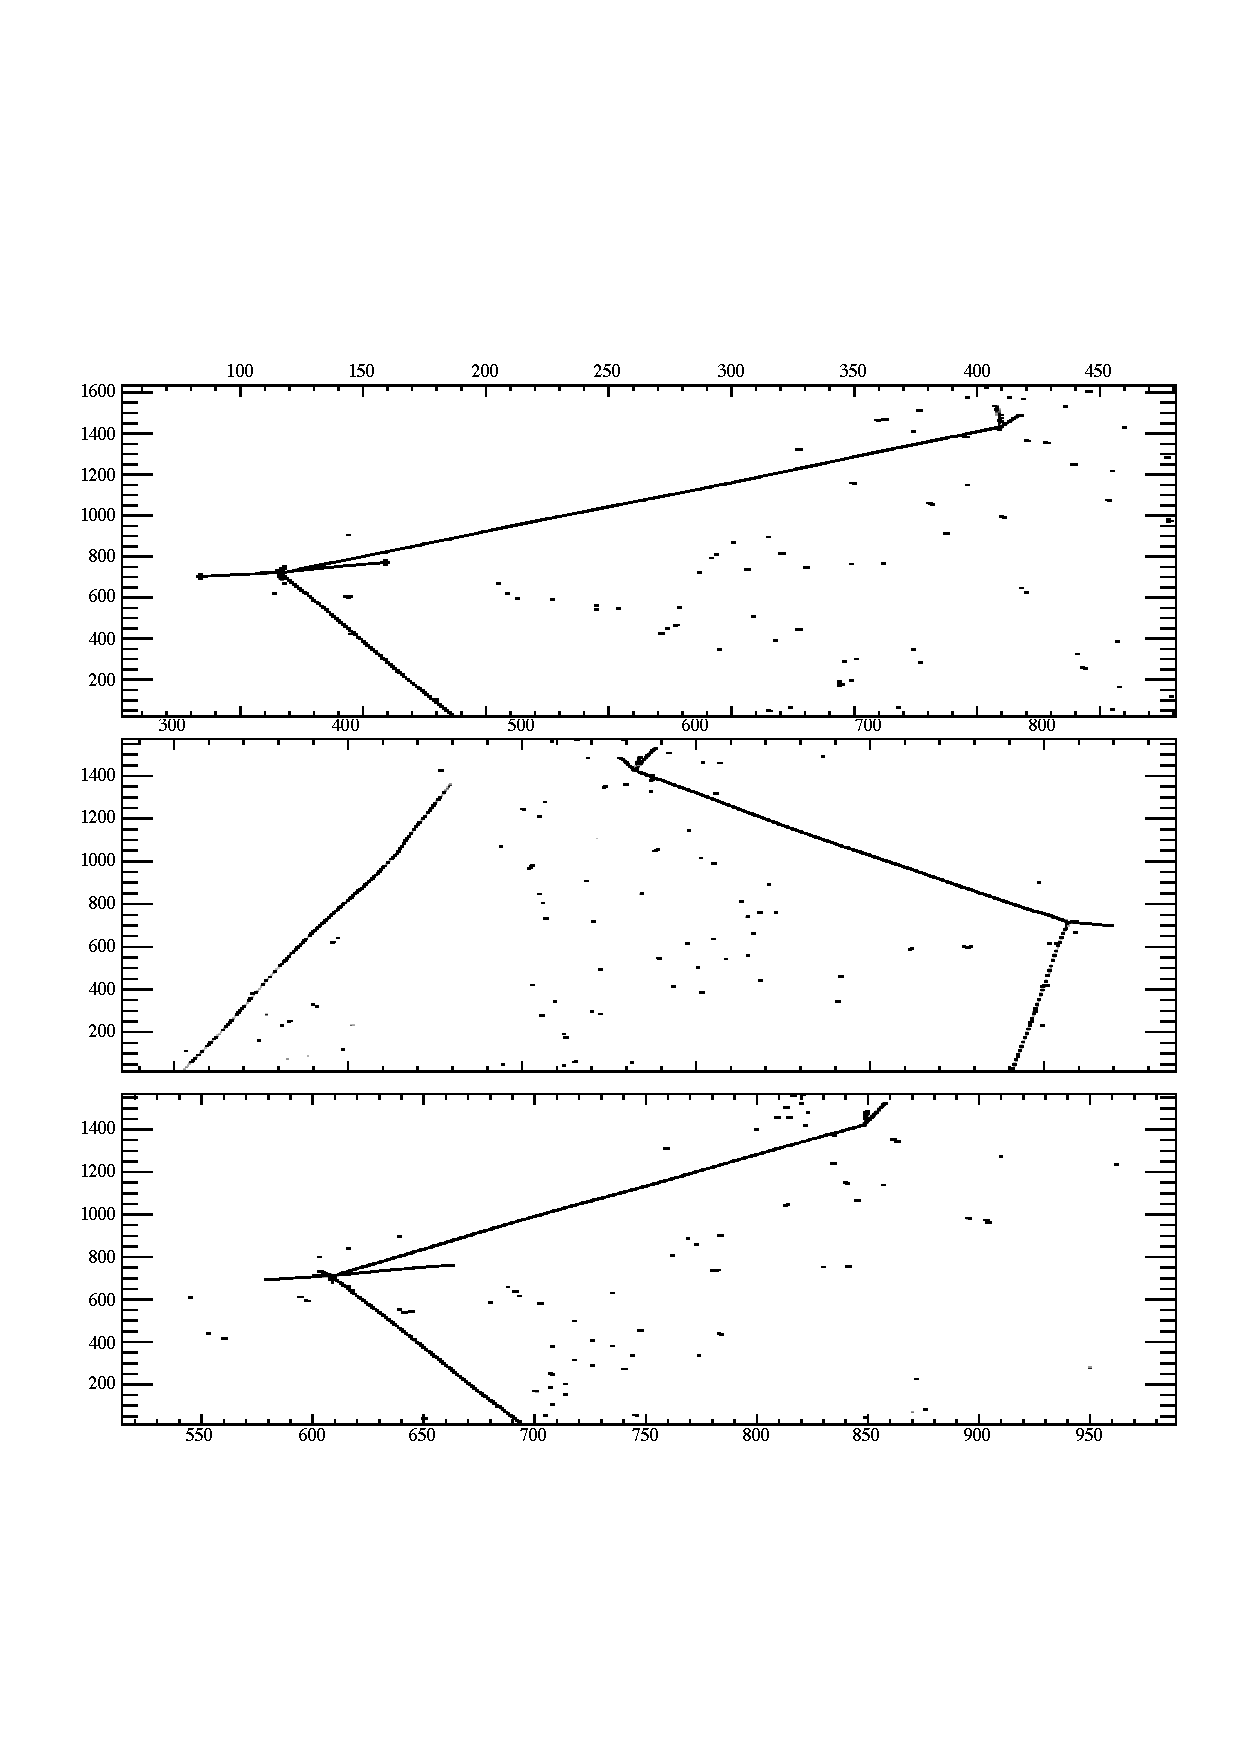
\includegraphics[width=0.98\textwidth]{2DnumuCCHits.pdf}
    \caption{Hit reconstruction.}
    \label{fig:2DnumuCCHits}
  \end{subfigure}
  \hfill
  \begin{subfigure}[t]{0.48\linewidth}
    \centering
    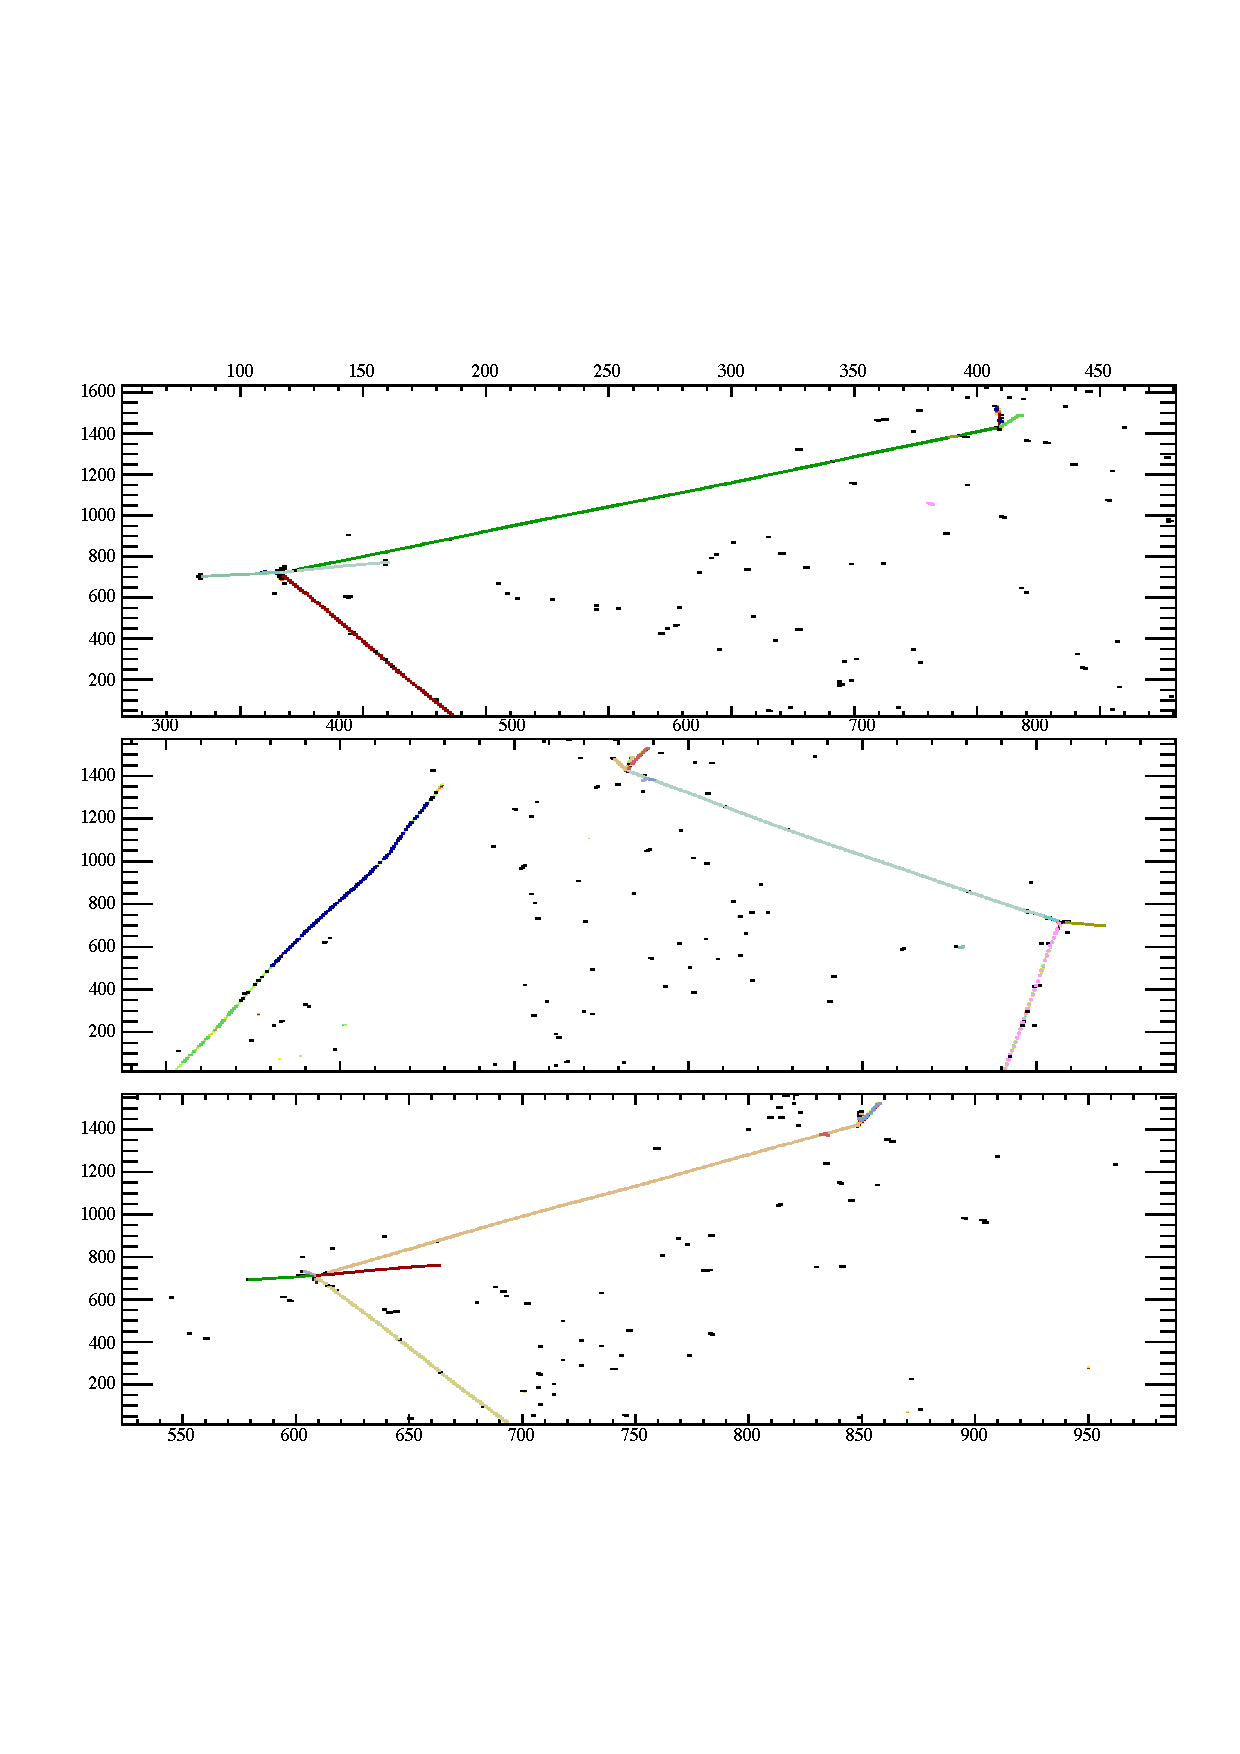
\includegraphics[width=0.98\textwidth]{2DnumuCCClusters.pdf}
    \caption{Cluster reconstruction.}
    \label{fig:2DnumuCCClusters}
  \end{subfigure}
  \caption[Demonstration of 2D reconstruction in LArSoft on a simulated $\nu_{\mu}$CC event.]{Demonstration of 2D reconstruction in LArSoft on a simulated $\nu_{\mu}$CC event.  The result of hit finding is shown in Figure~\ref{fig:2DnumuCCHits}, where each black rectangle represents a separate hit, and the grouping of these hits into clusters is illustrated in Figure~\ref{fig:2DnumuCCClusters}, where blocks of hits sharing a common colour are associated to the same cluster object.}
  \label{fig:2DnumuCC}
\end{figure}

Combining 2D information from multiple views in a LArTPC enables the formation of 3D objects.  In LArSoft, several 3D products exist: `space points', `vertices', `tracks' and `showers'.  Space points are a form of 3D hit, defined simply by a point in the detector Cartesian geometry, and vertices are a specific example of these locations created to represent an important part of the event (e.g. the neutrino interaction point or even just a track start).  Tracks and showers are more complete objects which represent individual particles and contain associated properties relevant to the topology of each.  Tracking is relatively advanced in LArSoft, with multiple track fitters shown to produce well-formed track objects efficiently; shower reconstruction is less so and will be discussed in detail in Section~\ref{sec:ShowerReconstruction}.

The result of applying track reconstruction to the $\nu_{\mu}$CC interaction discussed in Figure~\ref{fig:2DnumuCC} is shown in Figure~\ref{fig:3DnumuCC}.  As with clusters, each colour represents a unique track object and it is clear from Figure~\ref{fig:3DnumuCC2D} that hits across multiple planes contribute to a given track.  A complementary view is also shown in Figure~\ref{fig:3DnumuCC3D}, where the objects are represented in two orthogonal views in the detector coordinate system.  The track finder used here is Projection Matching Algorithm (PMA) \cite{PMA2013}.

\begin{figure}
  \centering
  \begin{subfigure}[t]{0.48\linewidth}
    \centering
    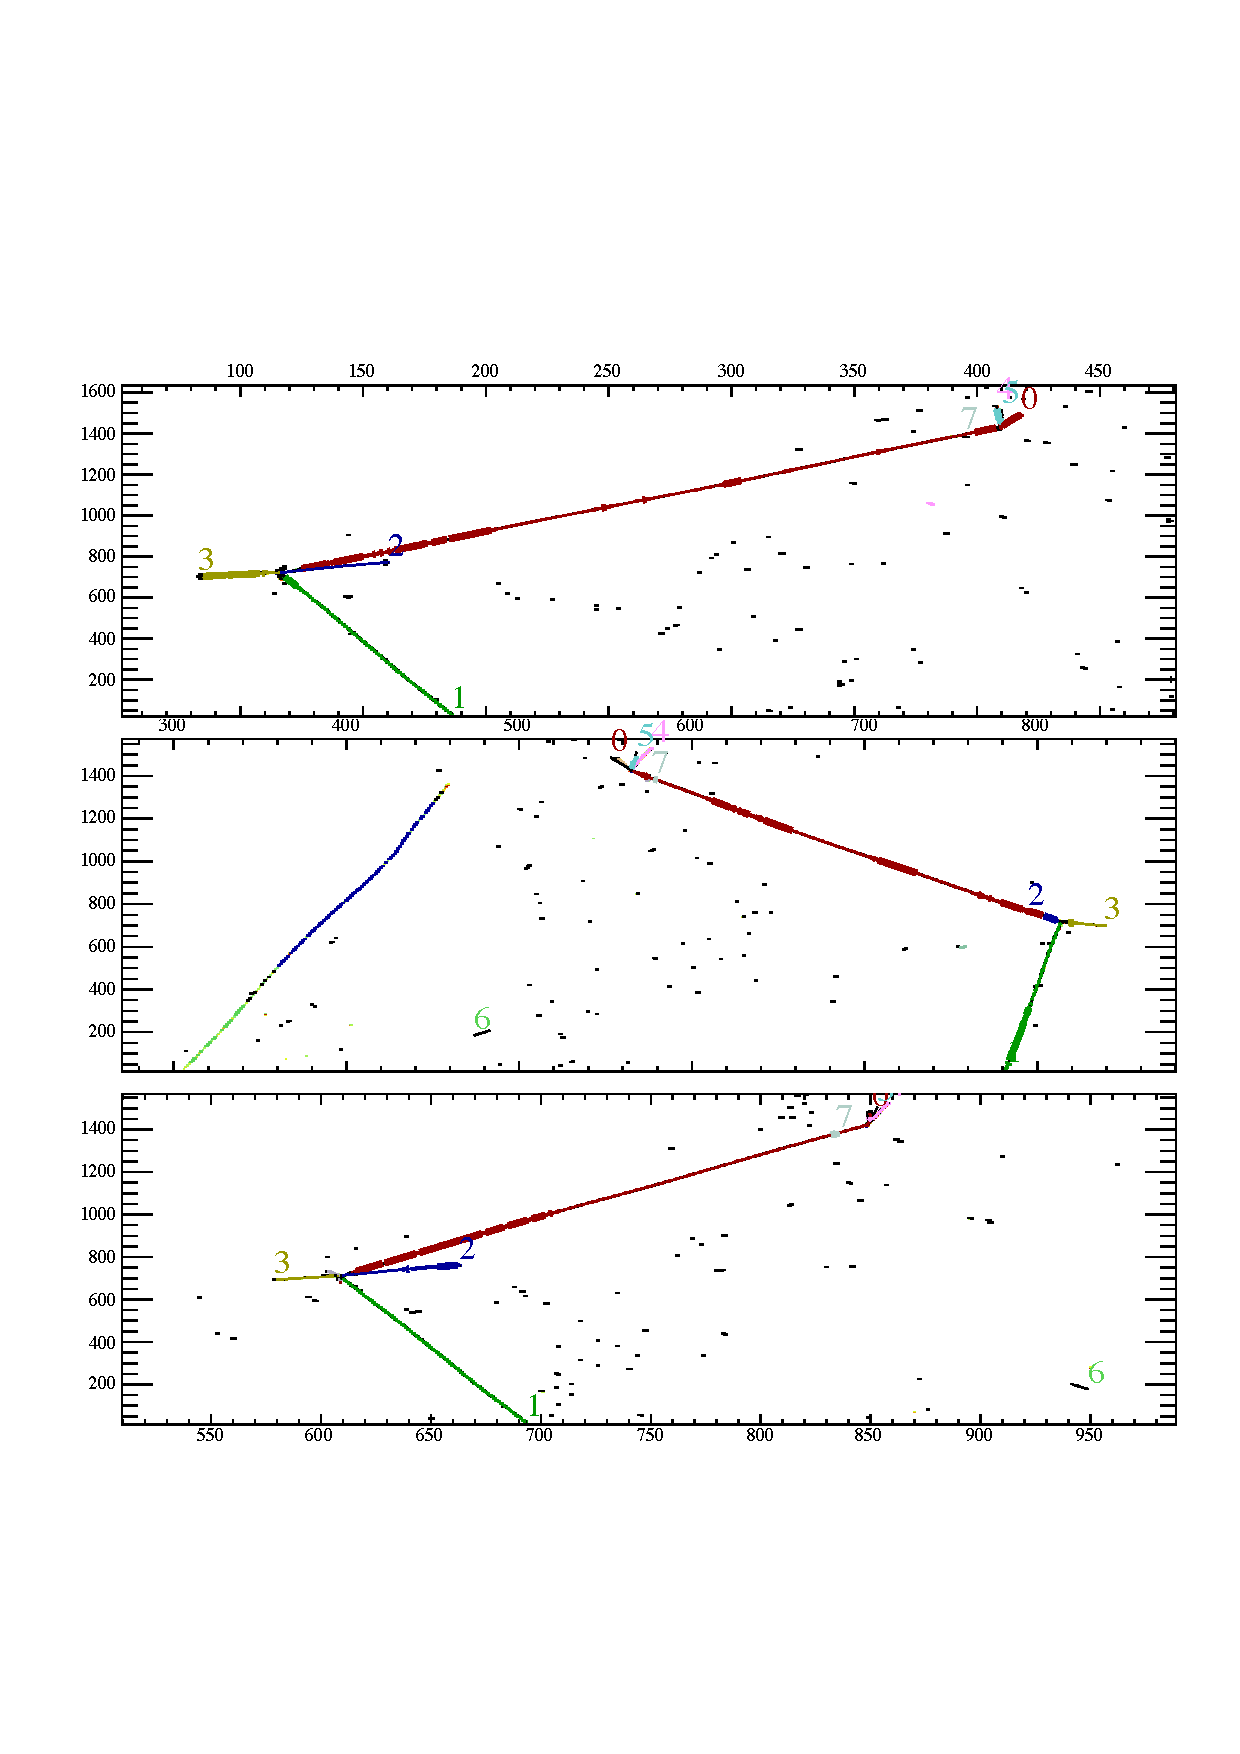
\includegraphics[width=0.98\textwidth]{3DnumuCC2D.pdf}
    \caption{2D view; wire vs tick for multiple wire planes.}
    \label{fig:3DnumuCC2D}
  \end{subfigure}
  \hfill
  \begin{subfigure}[t]{0.48\linewidth}
    \centering
    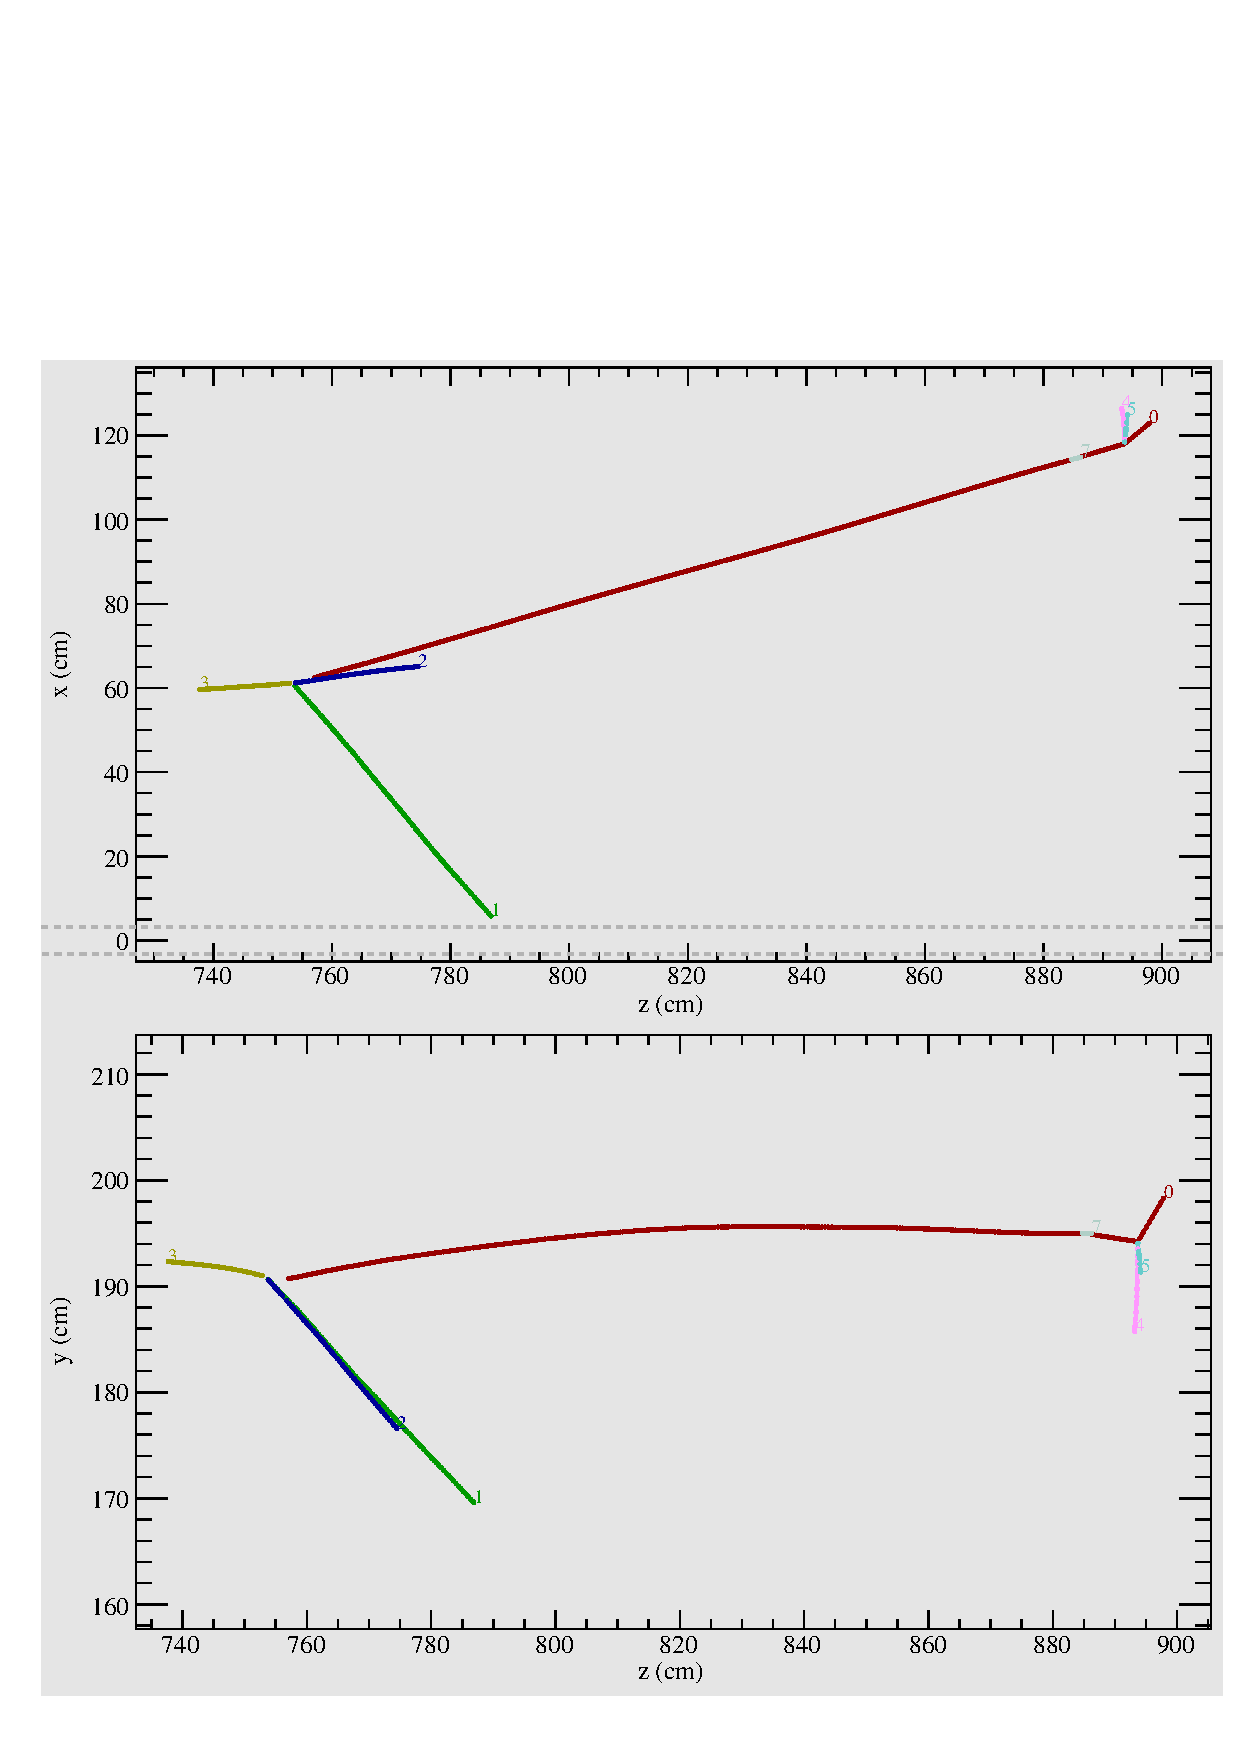
\includegraphics[width=0.98\textwidth]{3DnumuCC3D.pdf}
    \caption{3D view; $x$-$z$ and $y$-$z$ orthogonal planes.}
    \label{fig:3DnumuCC3D}
  \end{subfigure}
  \caption[Demonstration of 3D reconstruction in LArSoft on a simulated $\nu_{\mu}$CC event.]{Demonstration of 3D reconstruction in LArSoft on a simulated $\nu_{\mu}$CC event.  Each colour represents a unique 3D track object, with information shared between each of the anode planes; this is evident in Figure~\ref{fig:3DnumuCC2D}.  An additional view is demonstrated in Figure~\ref{fig:3DnumuCC3D} where two orthogonal planes of the detector geometry are shown.}
  \label{fig:3DnumuCC}
\end{figure}

It is worth noting the approach to forming the eventual 3D objects, from which particle identification and analysis may be executed, is not unique.  The method outlined above is most relevant to the shower reconstruction discussed in Section~\ref{sec:ShowerReconstruction} and is the most common chain used in most LArSoft processing; however, progress is being made on an additional technique which focusses directly on 3D reconstruction.  This is called `Wire-Cell' \cite{WireCellWebsite} and utilises a tomographic method, following the LArTPC principle that each plane observes the same amount of ionisation electrons, to build up a 3D image of the event.  This may then be characterised to find the properties of the particles and make the track and shower products.  All reconstruction methods utilise the same information provided by the detector but not necessarily in the same order.

%----------------------------------------------------------------------------------------------------------------------------------------------------------------------------
\subsection{Calorimetry}\label{sec:Calorimetry}

The possibility of extremely precise energy measurements is a hugely attractive feature of LArTPCs and is achieved by careful calibration of the charge received from the drift electrons.  There are a number of distinct calibrations which must be conducted to ensure reliable calorimetric measurements and the relevant procedures will be outlined in this section.  Setting the ADC to energy translation is the subject of Section~\ref{sec:EnergyDetermination} and determining the electromagnetic shower and neutrino energy conversion from the total deposited charge will be discussed in Sections~\ref{sec:ShowerEnergy} and~\ref{sec:NeutrinoEnergy} respectively.

%----------------------------------------------------------------------------------------------------------------------------------------------------------------------------
\subsubsection{Energy Determination}\label{sec:EnergyDetermination}

Following deconvolution and hit finding, the charge carried by each packet of electrons is understood as the Gaussian integral of the hit and is normalised, by default, in units of 200~e$^-$ (often just `ADC' in certain following plots).  The `calorimetry constant', responsible for converting between digitised readout charge and the number of electrons which deposited the charge, is therefore $5\times10^{-3}$ in simulation (1/200), but is not necessarily equivalent in data due to limitations of the simulation.  This will be discussed further in Section~\ref{sec:DataCalorimetryReconstruction} in Chapter~\ref{chap:35tonAnalysis}.

The precise calorimetry constant may be tuned by considering minimally ionising particles (mips), which are known to deposit 2.1~MeV/cm energy when propagating through LAr.  The number of electrons contributing to a hit is determined using the calorimetry constant and corrected for lifetime and recombination to yield the total number of ionised electrons initially forming the ionisation packet.  Utilising the ionisation energy of LAr (23.6~eV/ion), the total energy deposited by the particle may be inferred.  Combining this information for hits on successive wires, accounting for the pitch of the particle track, enables a measurement of dE/dx to be made.  By plotting the distribution for multiple tracks, the calorimetry constant may be tuned until the dE/dx is as expected.

%----------------------------------------------------------------------------------------------------------------------------------------------------------------------------
\subsubsection{Shower Energy Reconstruction}\label{sec:ShowerEnergy}

For large groups of hits from a common source, such as for electromagnetic showers, an alternative approach may be employed.  A linear correlation is observed between the lifetime-corrected charge deposited and the true deposited energy energy, demonstrated in Figure~\ref{fig:ShowerEnergyConversion}.  This was made by simulating 1000 electrons in the DUNE far detector geometry at each of the energies 0.5,~1.0,~...,~5.0~GeV and taking a Gaussian fit of the total charge deposited in the detector for each energy.  An almost-perfect linear fit is observed and the associated parameters are used when determining the shower energy in reconstruction.

\begin{figure}
  \centering
  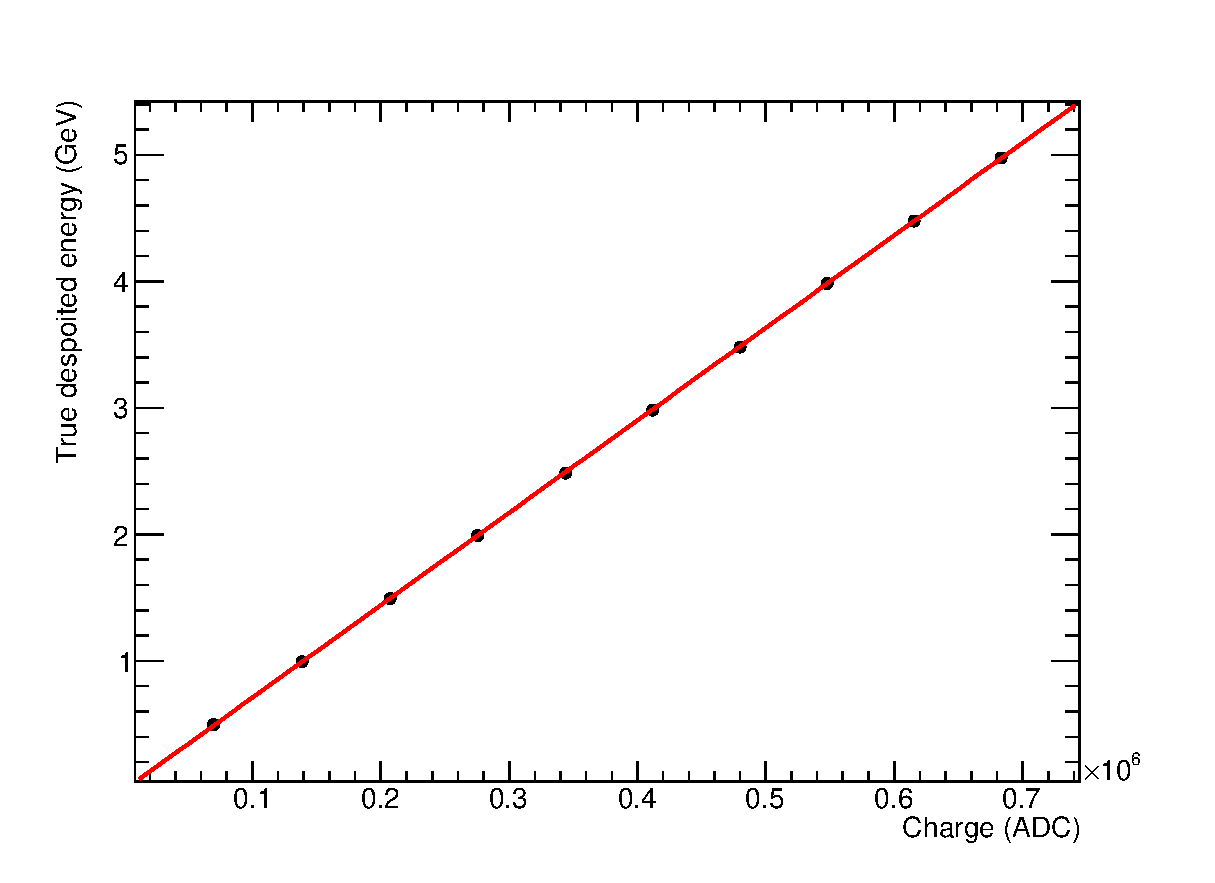
\includegraphics[width=10cm]{ShowerEnergyConversionFD.eps}
  \caption[Correlation between the true deposited energy in an electromagnetic shower and the total charge in the detector for electron showers in the DUNE far detector.]{Correlation between the true deposited energy in an electromagnetic shower and the total charge in the detector for electron showers in the DUNE far detector.  The parameters from the linear fit are extracted for use in the reconstruction.}
  \label{fig:ShowerEnergyConversion}
\end{figure}

%----------------------------------------------------------------------------------------------------------------------------------------------------------------------------
\subsubsection{Neutrino Energy Reconstruction}\label{sec:NeutrinoEnergy}

In order to reconstruct the neutrino energy from beam interactions, a similar approach to the method discussed in Section~\ref{sec:ShowerEnergy} is employed on the hadronic activity in the detector \cite{Grant2017}.  Leptonic energy (i.e. muon tracks and electron showers) is determined separately and subtracted from the total energy, leaving the charge deposited from hadrons which may be converted to deposited energy using the linear relationship.  This approach ensures the correct calibration for the hadronic energy, which often includes unseen contributions from neutrons.  The lepton energy is determined either from the electron shower energy or, in the case of a muon, by using either containment or multiple Coulomb scattering (MCS) considerations.

%----------------------------------------------------------------------------------------------------------------------------------------------------------------------------
\section{Shower Reconstruction in LArTPCs}\label{sec:ShowerReconstruction}

Reconstructing showers in a LArTPC is challenging and until recently was an unsolved problem in LArSoft.  This section describes the development of novel techniques for the purposes of complete shower reconstruction within a LArTPC.  The primary motivations for the undertaking were initially the desire to perform a $\pi^0$ analysis in the 35~ton dataset and the lack of available tools.  The reconstruction was thus developed with $\pi^0$s in mind, specifically focussing on the separation of closely occurring showers from the two photon daughters, but has utility in the reconstruction of all showering particles.

Excellent shower reconstruction is essential for the success of the DUNE experiment.  In order to distinguish between the main oscillation signal (discussed further in Chapter~\ref{chap:FDAnalysis})
\begin{equation}
  \nu_e + n \rightarrow e^- + p^+
\end{equation}
and the potentially tricky neutral current background
\begin{equation}
  \nu_{\mu} + n \rightarrow \nu_{\mu} + \pi^0 + \textnormal{hadrons},
\end{equation}
the electron and the $\pi^0$ decay photons must be well discriminated.  This motivates the requirement of high quality reconstruction of these electromagnetically showering particles.

The shower reconstruction problem is first overviewed in Section~\ref{sec:ShowersOverview} before the specific algorithms are discussed in Sections~\ref{sec:BlurredCluster} and~\ref{sec:EMShower} respectively.  A further problem in LArTPC reconstruction, track/shower separation, is the subject of Section~\ref{sec:TrackShowerSeparation}, before finally the performance of the reconstruction is evaluated in Section~\ref{sec:ReconstructionPerformance}.

%----------------------------------------------------------------------------------------------------------------------------------------------------------------------------
\subsection{Showers Overview}\label{sec:ShowersOverview}

High energy electrons and photons produce electromagnetic showers in a LArTPC via pair production and bremsstrahlung processes.  They may be distinguished using the excellent calorimetric properties of the detector by careful analysis of the initial part of the object, before showering occurs.  A photon, since it has no electric charge, does not ionise and so is only observable following pair production.  Thus, one would expect the initial part of a photon shower to be twice as ionising (two electrons) than the start of an electron shower (a single electron); the dE/dx at the beginning of an electron and a photon shower is 2.1~MeV/cm and 4.2~MeV/cm respectively.

The required properties provided by the reconstruction of electromagnetic showers include an accurate start position and direction, a dE/dx measurement for the first 3~cm of the shower and the total deposited energy left by the shower.  It is thus vital the object is as complete as possible and is orientated correctly.  Additionally, good separation between $\pi^0$ decay photon showers is required for calibration purposes and to reduce the neutral current $\pi^0$ backgrounds previously discussed.  An example 35~ton particle gun $\pi^0$ event is shown in Figure~\ref{fig:pi0Showers} to demonstrate the task presented to the reconstruction.

\begin{figure}
  \centering
  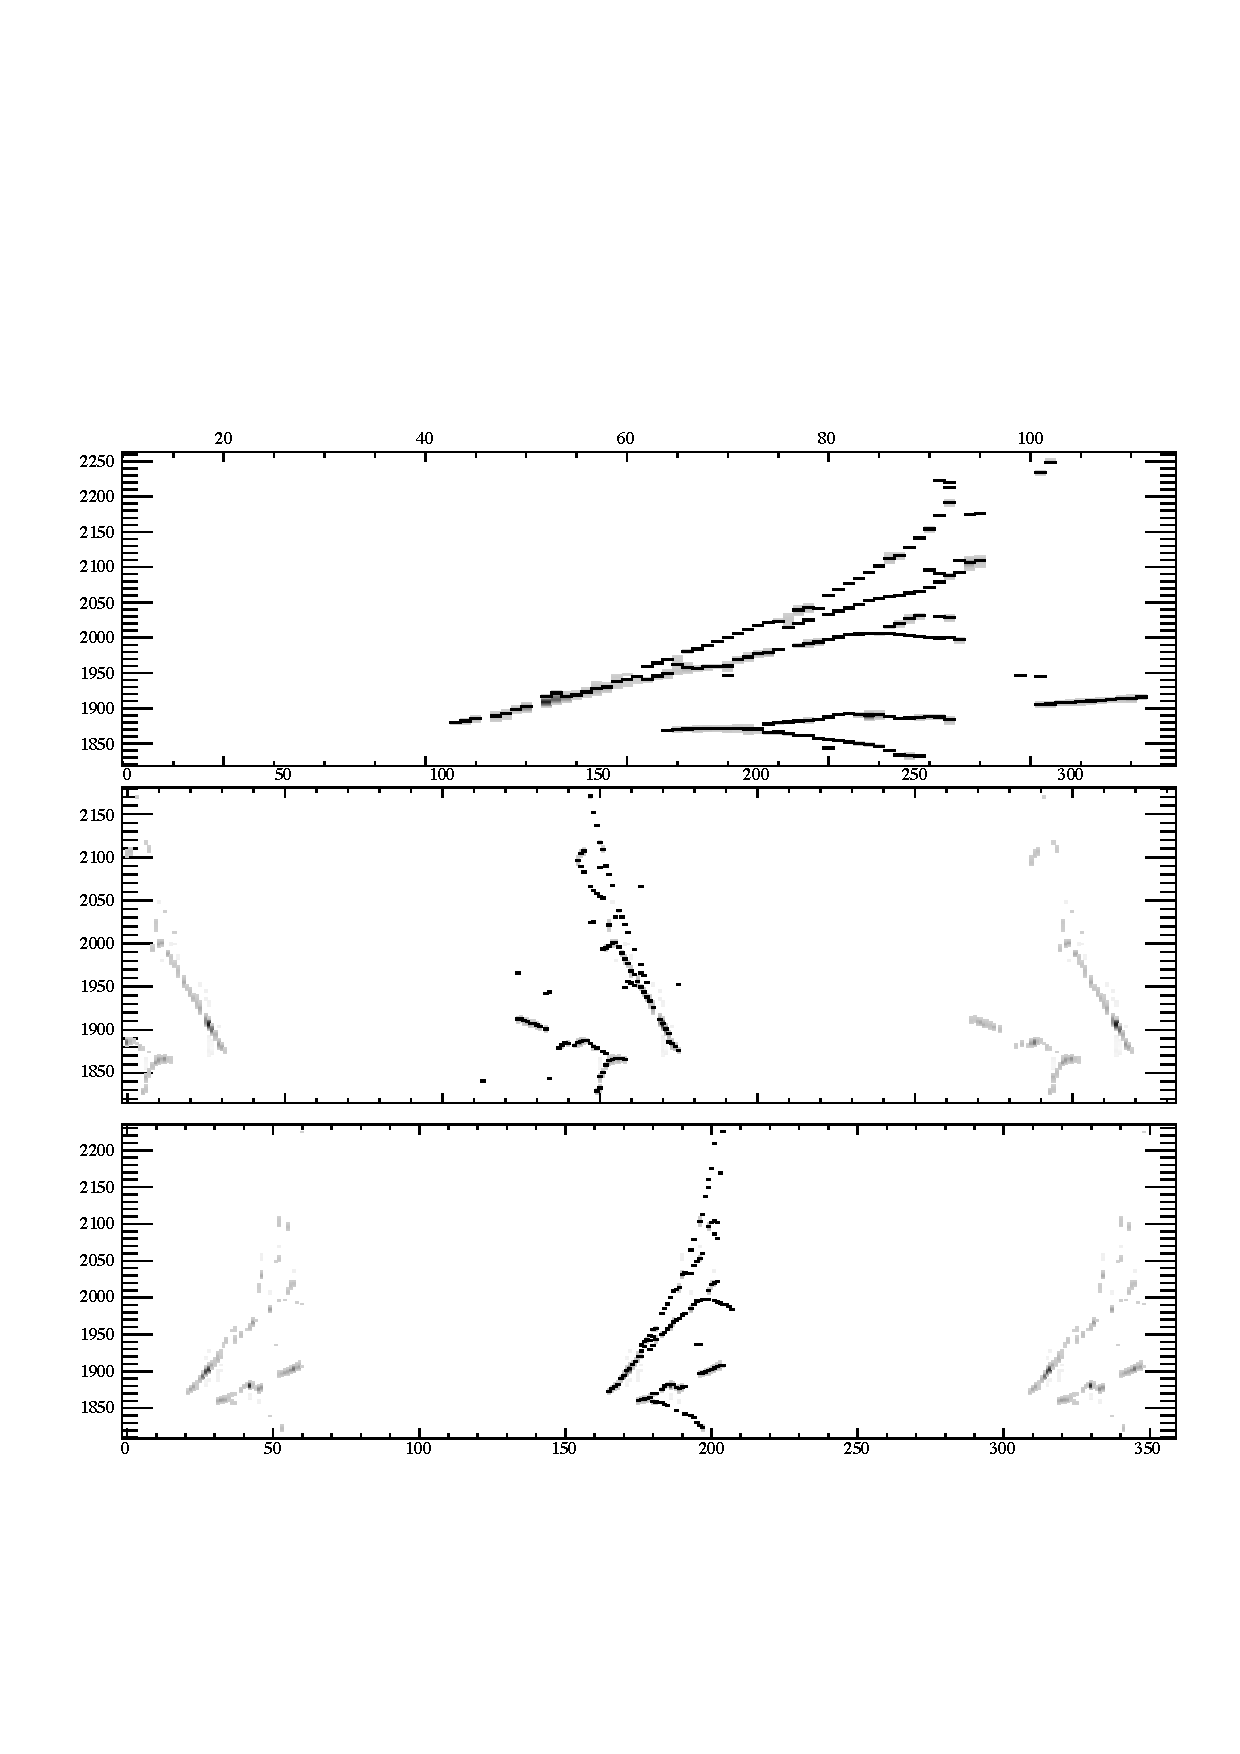
\includegraphics[width=10cm]{EVDPi0Hits.pdf}
  \caption[An example particle gun $\pi^0$ event in the 35~ton geometry.]{An example particle gun $\pi^0$ event in the 35~ton geometry.  Hit reconstruction (including disambiguation in the induction planes) has been applied with individual hits shown as black rectangles.  The two decay photons are visible by eye but shower very close to each other.}
  \label{fig:pi0Showers}
\end{figure}

The algorithms presented in the following section successfully meet these criteria and produce high quality reconstructed showers with high efficiency.  Two methods are outlined, BlurredCluster and EMShower, which are designed to perform 2D and 3D reconstruction respectively and together produce fully reconstructed shower objects.

%----------------------------------------------------------------------------------------------------------------------------------------------------------------------------
\subsection{BlurredCluster Algorithm}\label{sec:BlurredCluster}

The BlurredCluster algorithm is a 2D clustering algorithm \cite{KabothThesis} implemented with LArSoft \cite{BlurredCluster,BlurredClusterLArSoft}.  It is optimised for shower reconstruction in general and, more specifically, for the reconstruction of $\pi^0$s.  The method convolves the hit map with a Gaussian kernel in order to `smear' out the deposited charge and introduce `fake' hits to facilitate a more complete and accurate reconstruction.

%----------------------------------------------------------------------------------------------------------------------------------------------------------------------------
\subsubsection{Algorithm Description}\label{sec:BlurredClusterDescription}

The energy deposited by showering particles is contained on several discrete readout wires which are not necessarily representative of the initial deposition of charge, which is more diffuse.  This motivates the concept of `smearing' the charge between adjacent wires, reproducing the more realistic distribution.  In addition, since ionisation packets naturally spread in time (longitudinal diffusion), it is natural to take this into account when redistributing the deposited energy.

The smearing is performed using a 2D Gaussian kernel, given by
\begin{equation}\label{eq:2DGaussianKernel}
  \frac{1}{\sqrt{2\pi}\sigma_{\textnormal{wire}}} \frac{1}{\sqrt{2\pi}\sigma_{\textnormal{tick}}} e^{-\frac{r_{\textnormal{wire}}^2}{2\sigma_{\textnormal{wire}}^2}} e^{-\frac{r_{\textnormal{tick}}^2}{2\sigma_{\textnormal{tick}}^2}}
\end{equation}
and defined by two parameters in each dimension (wire and tick); the standard deviation $\sigma$ of the Gaussian function and the `blurring radius' $r$, the distance the blurring is extended in each direction.  An example of such a kernel is demonstrated in Figure~\ref{fig:2DGaussianKernel}.

\begin{figure}
  \centering
  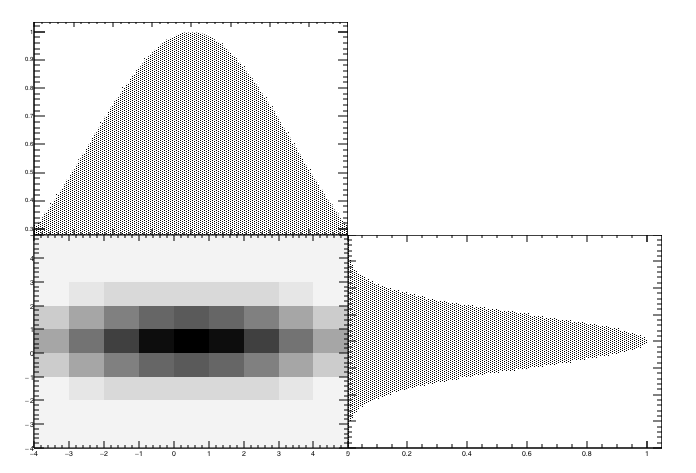
\includegraphics[width=10cm]{2DGaussianKernel.png}
  \caption[A example 2D Gaussian kernel alongside the contributions from each dimension.]{A example 2D Gaussian kernel, made using Equation~\ref{eq:2DGaussianKernel}, alongside the contributions from each dimension.  In the context of convolving with a hit map for reconstruction purposes, consider the charge at point (0, 0) to be a hit.  The neighbouring bins, within a given blurring radius $r$ (in this case, 4 in each direction), are assigned charge according to the value of the kernel at each point.  If no charge were originally deposited at that location, a `fake' hit is introduced.  In this example, the Gaussian in the horizontal direction is much wider ($\sigma=2.6$) than in the vertical direction ($\sigma=1$).}
  \label{fig:2DGaussianKernel}
\end{figure}

The Gaussian widths and blurring radii in each direction are determined dynamically for each individual hit map and even for individual hits.  This is achieved by initially guessing a direction of each shower (using least squares and Principal Component Analysis (PCA) considerations) and assigning the parameters values relevant to the assumed directionality.  For example, if it appears a particle shower is travelling primarily in the wire direction, an appropriate 2D kernel would be wider in the wire direction and would extend further in this dimension (i.e. $r_{\textnormal{wire}} \gg r_{\textnormal{tick}}$).  This example is demonstrated in Figure~\ref{fig:2DGaussianKernel} where it is clear the charge is noticeably smeared more in the wire (horizontal) than the tick (vertical) direction.  Additionally, the width of a particular hit in time is taken into account when selecting an appropriate kernel with which to smear its charge.  A hit with a greater width justifies a much wider kernel in the tick direction to take into account this distribution of charge.

A demonstration, in 1D, of the convolution process is the subject of Figure~\ref{fig:BlurringProcess}.  In this example, the width of the kernel is fixed and the blurring radius is set to 2.  The final charge distribution may be compared to the input hit map in the bottom right figure, in which a more realistic smearing of the deposited energy in the detector may be observed.  The process in 2D is identical to this simplified example but uses contributions from bins in two dimensions rather than just one.

\begin{figure}
  \centering
  \begin{subfigure}[t]{0.3\linewidth}
    \centering
    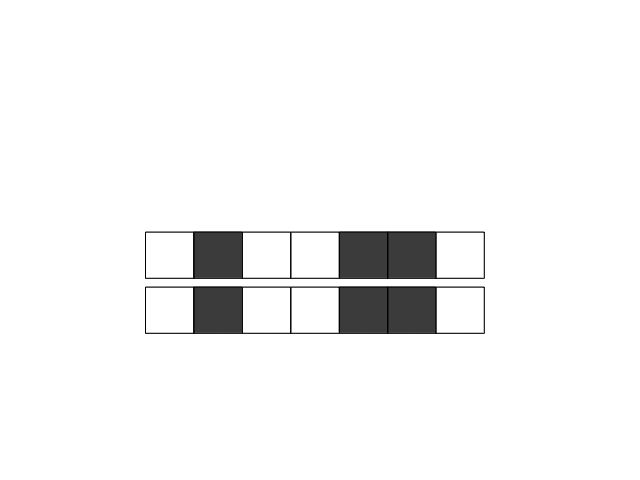
\includegraphics[width=\textwidth]{blurring1.png}
    %\caption{}
  \end{subfigure}
  \hfill
  \begin{subfigure}[t]{0.3\linewidth}
    \centering
    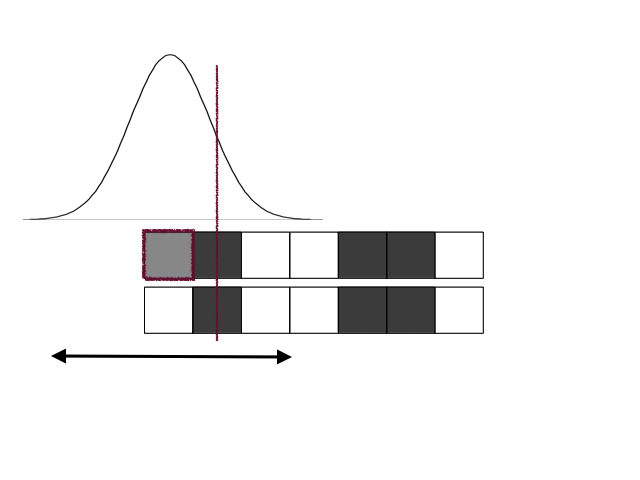
\includegraphics[width=\textwidth]{blurring2.png}
    %\caption{}
  \end{subfigure}
  \hfill
    \begin{subfigure}[t]{0.3\linewidth}
    \centering
    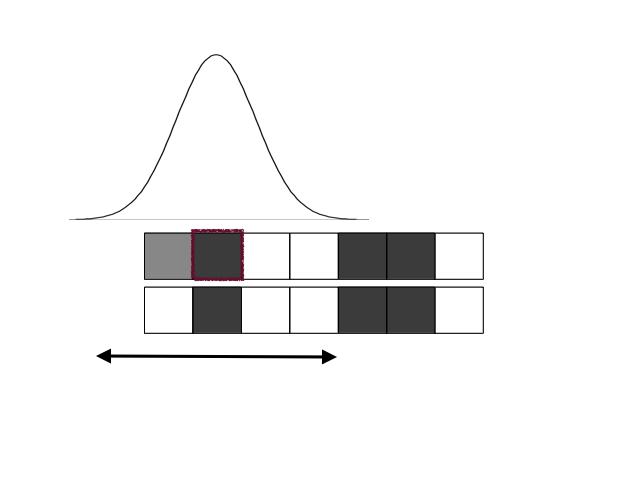
\includegraphics[width=\textwidth]{blurring3.png}
    %\caption{}
  \end{subfigure}
  \vfill
  \begin{subfigure}[t]{0.3\linewidth}
    \centering
    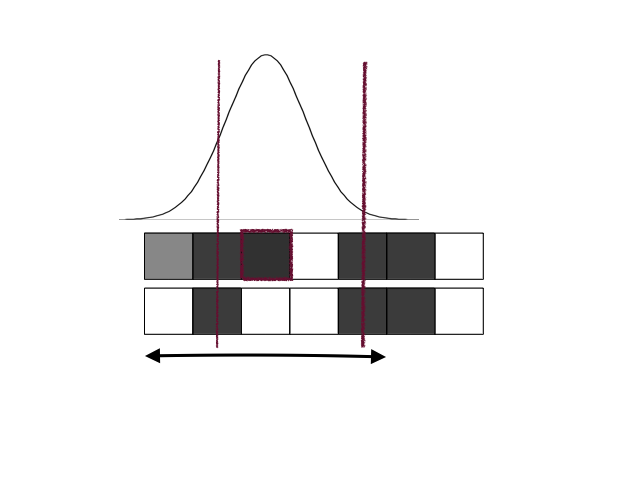
\includegraphics[width=\textwidth]{blurring4.png}
    %\caption{}
  \end{subfigure}
  \hfill
  \begin{subfigure}[t]{0.3\linewidth}
    \centering
    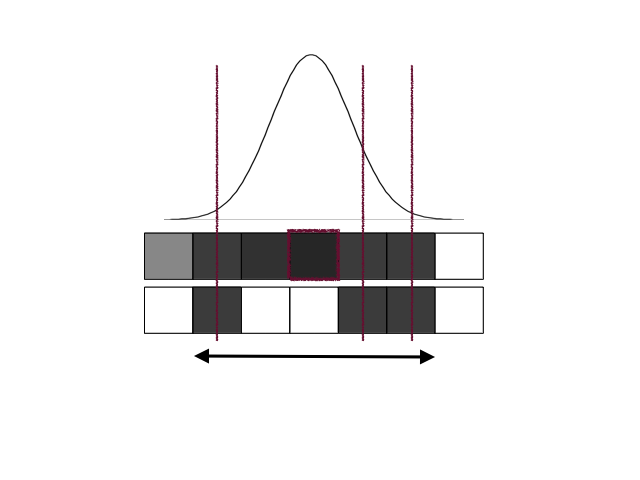
\includegraphics[width=\textwidth]{blurring5.png}
    %\caption{}
  \end{subfigure}
  \hfill
  \begin{subfigure}[t]{0.3\linewidth}
    \centering
    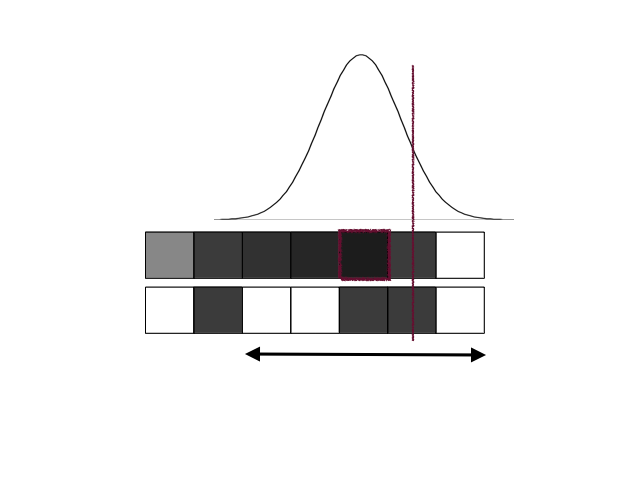
\includegraphics[width=\textwidth]{blurring6.png}
    %\caption{}
  \end{subfigure}
  \vfill
  \begin{subfigure}[t]{0.3\linewidth}
    \centering
    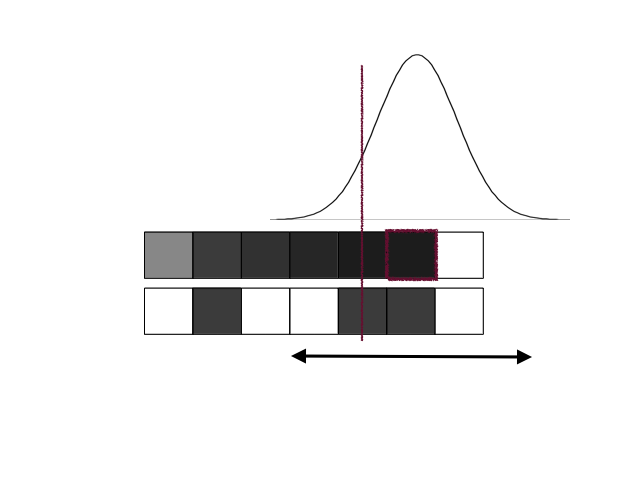
\includegraphics[width=\textwidth]{blurring7.png}
    %\caption{}
  \end{subfigure}
  \hfill
  \begin{subfigure}[t]{0.3\linewidth}
    \centering
    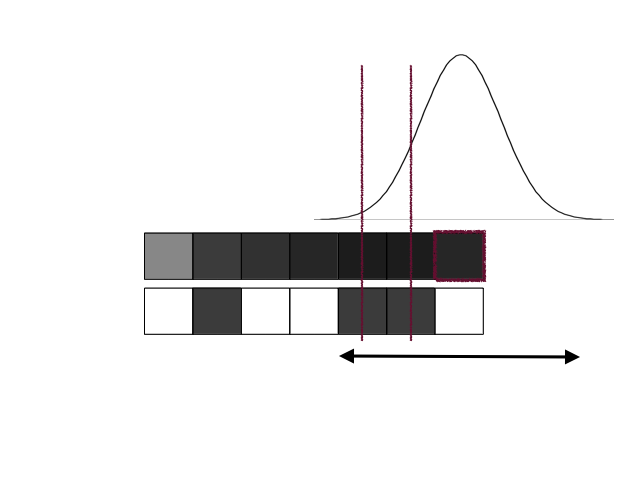
\includegraphics[width=\textwidth]{blurring8.png}
    %\caption{}
  \end{subfigure}
  \hfill
  \begin{subfigure}[t]{0.3\linewidth}
    \centering
    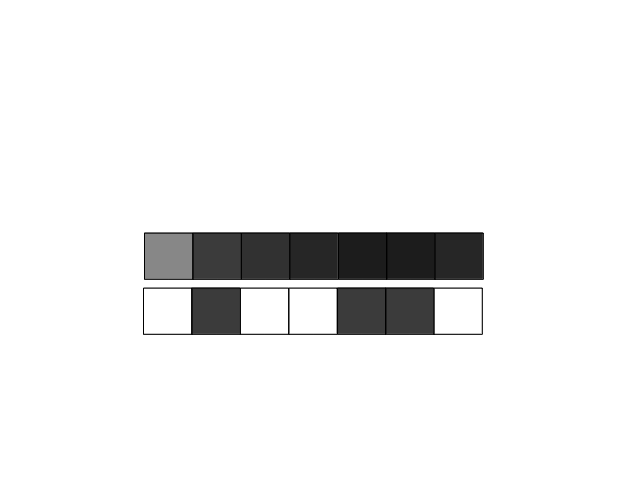
\includegraphics[width=\textwidth]{blurring9.png}
    %\caption{}
  \end{subfigure}
  \caption[Simplified demonstration, in 1D, of the blurring process used when smearing charge from a hit map.]{Simplified demonstration, in 1D, of the blurring process used when smearing charge from a hit map.  The process follows from left to right, top to bottom.  The Gaussian width is fixed for each hit and the blurring radius is set to 2.  For each bin, any real hits within the blurring radius (represented by red lines) contribute to the charge introduced as a fake hit.  The original hit map in shown underneath the blurred version, which is completed as the bins are looped through.  The final blurred hit map shows a nice smearing of the input charge according to the original distribution of charge and the particular Gaussian kernel used in the convolution.}
  \label{fig:BlurringProcess}
\end{figure}

The result of the Gaussian blurring process on the 35~ton $\pi^0$ depicted in Figure~\ref{fig:pi0Showers} is shown in Figure~\ref{fig:pi0ShowersBlurredMap}.  The efficacy with which the blurring encompasses the showers, whilst maintaining separation, is evident.  This is the aim for the smearing process and the resulting shower quality is directly dependent on how well the charge is redistributed before clustering.

\begin{figure}
  \centering
  \begin{subfigure}[t]{0.48\linewidth}
    \centering
    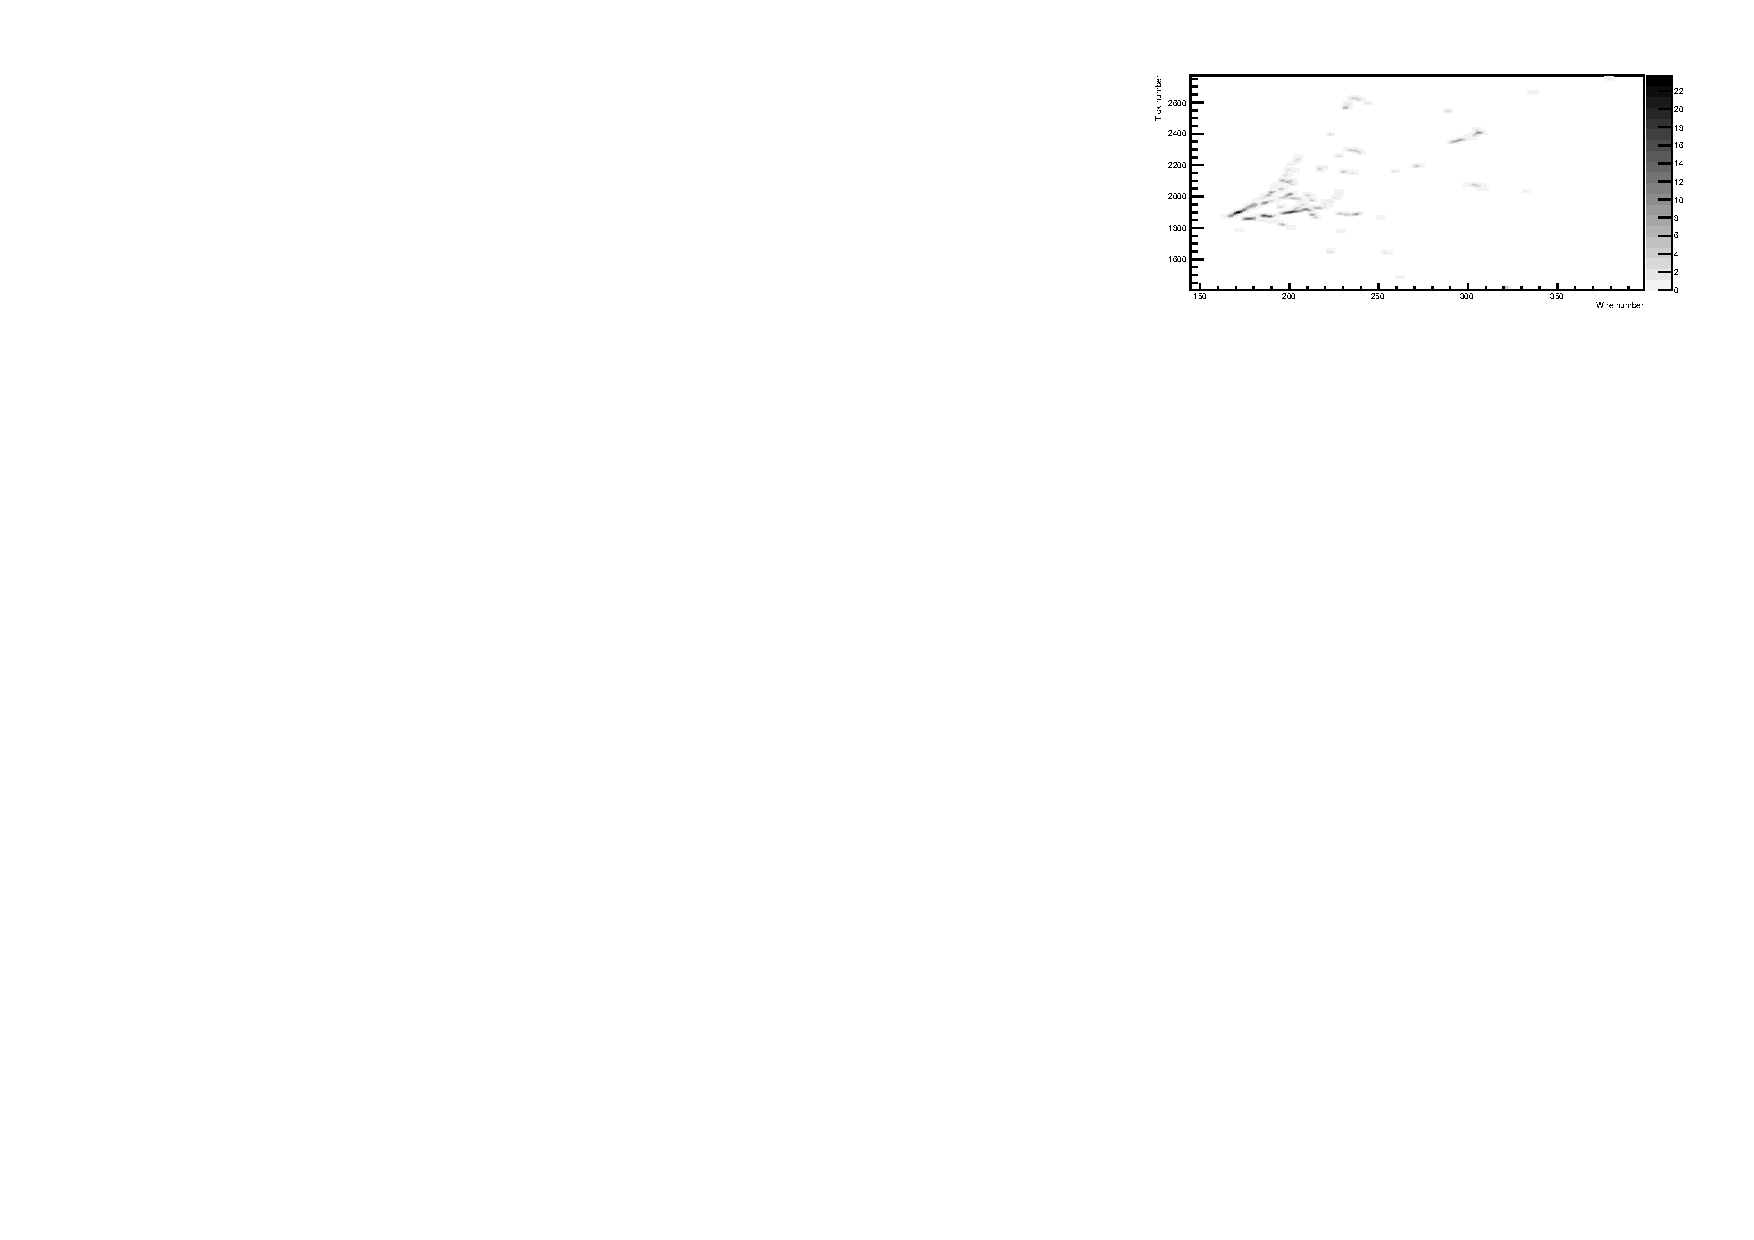
\includegraphics[width=0.98\textwidth]{EVDPi0BlurPlane0.pdf}
    \caption{Plane 0.}
    \label{fig:pi0ShowerBlurredMapPlane0}
  \end{subfigure}
  \hfill
  \begin{subfigure}[t]{0.48\linewidth}
    \centering
    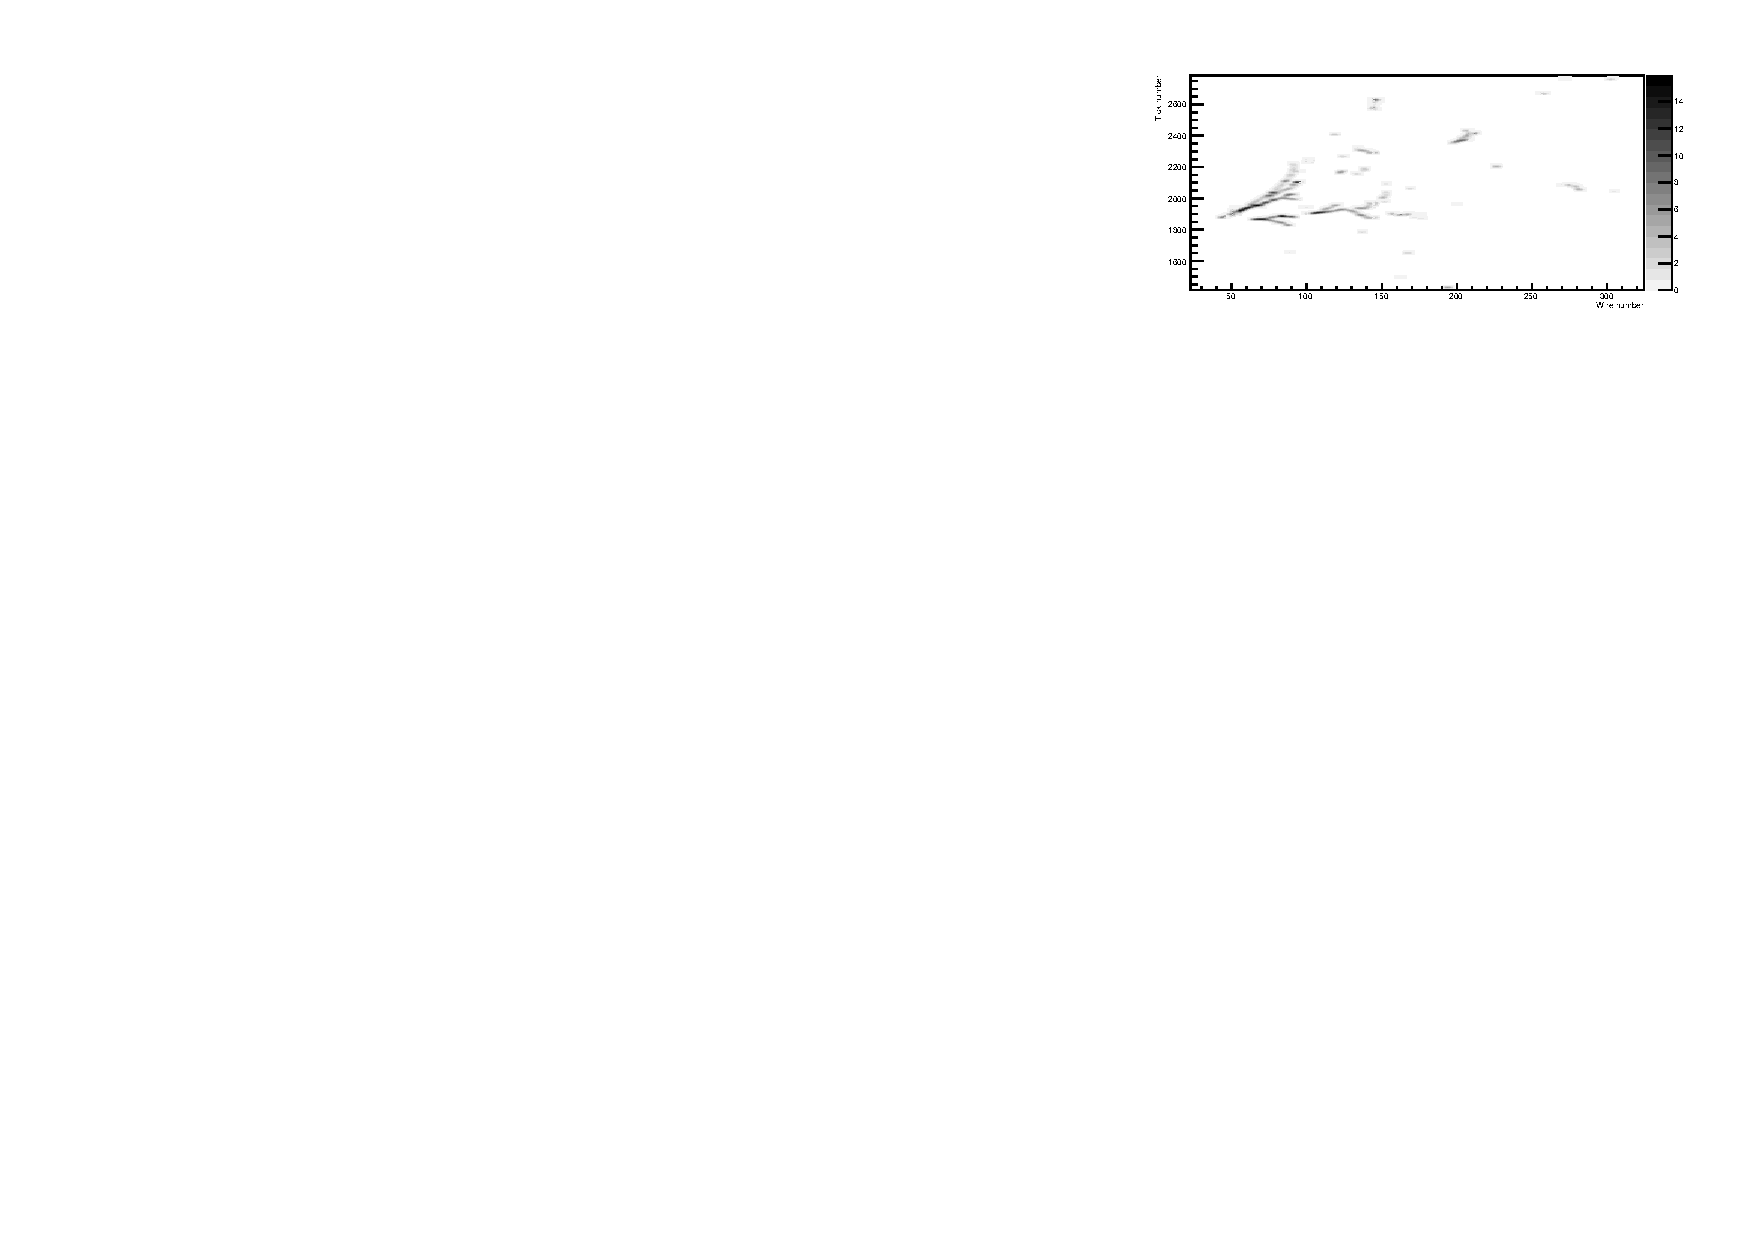
\includegraphics[width=0.98\textwidth]{EVDPi0BlurPlane2.pdf}
    \caption{Plane 2.}
    \label{fig:pi0ShowerBlurredMapPlane2}
  \end{subfigure}
  \caption[The output of the blurring stage of the BlurredCluster algorithm on the hit maps from two planes of the 35~ton $\pi^0$ event illustrated in Figure~\ref{fig:pi0Showers}.]{The output of the blurring stage of the BlurredCluster algorithm on the hit maps from two planes of the 35~ton $\pi^0$ event illustrated in Figure~\ref{fig:pi0Showers}.  The greyscale represents charge deposited in the wire/tick space.}
  \label{fig:pi0ShowersBlurredMap}
\end{figure}

Following completion of the hit map blurring, clustering proceeds utilising a simple nearest neighbour algorithm.  This is sufficient to group all hits of a shower together once the Gaussian smearing has smoothed out the charge distribution and introduced fake hits to populate gaps in the collected charge.  The final stage of the process involves identifying the original hits and producing the relevant output clusters for use in further algorithms.  The output clusters produced by the BlurredCluster algorithm for the 35~ton $\pi^0$ event are demonstrated in Figure~\ref{fig:pi0ShowersClusters}.

\begin{figure}
  \centering
  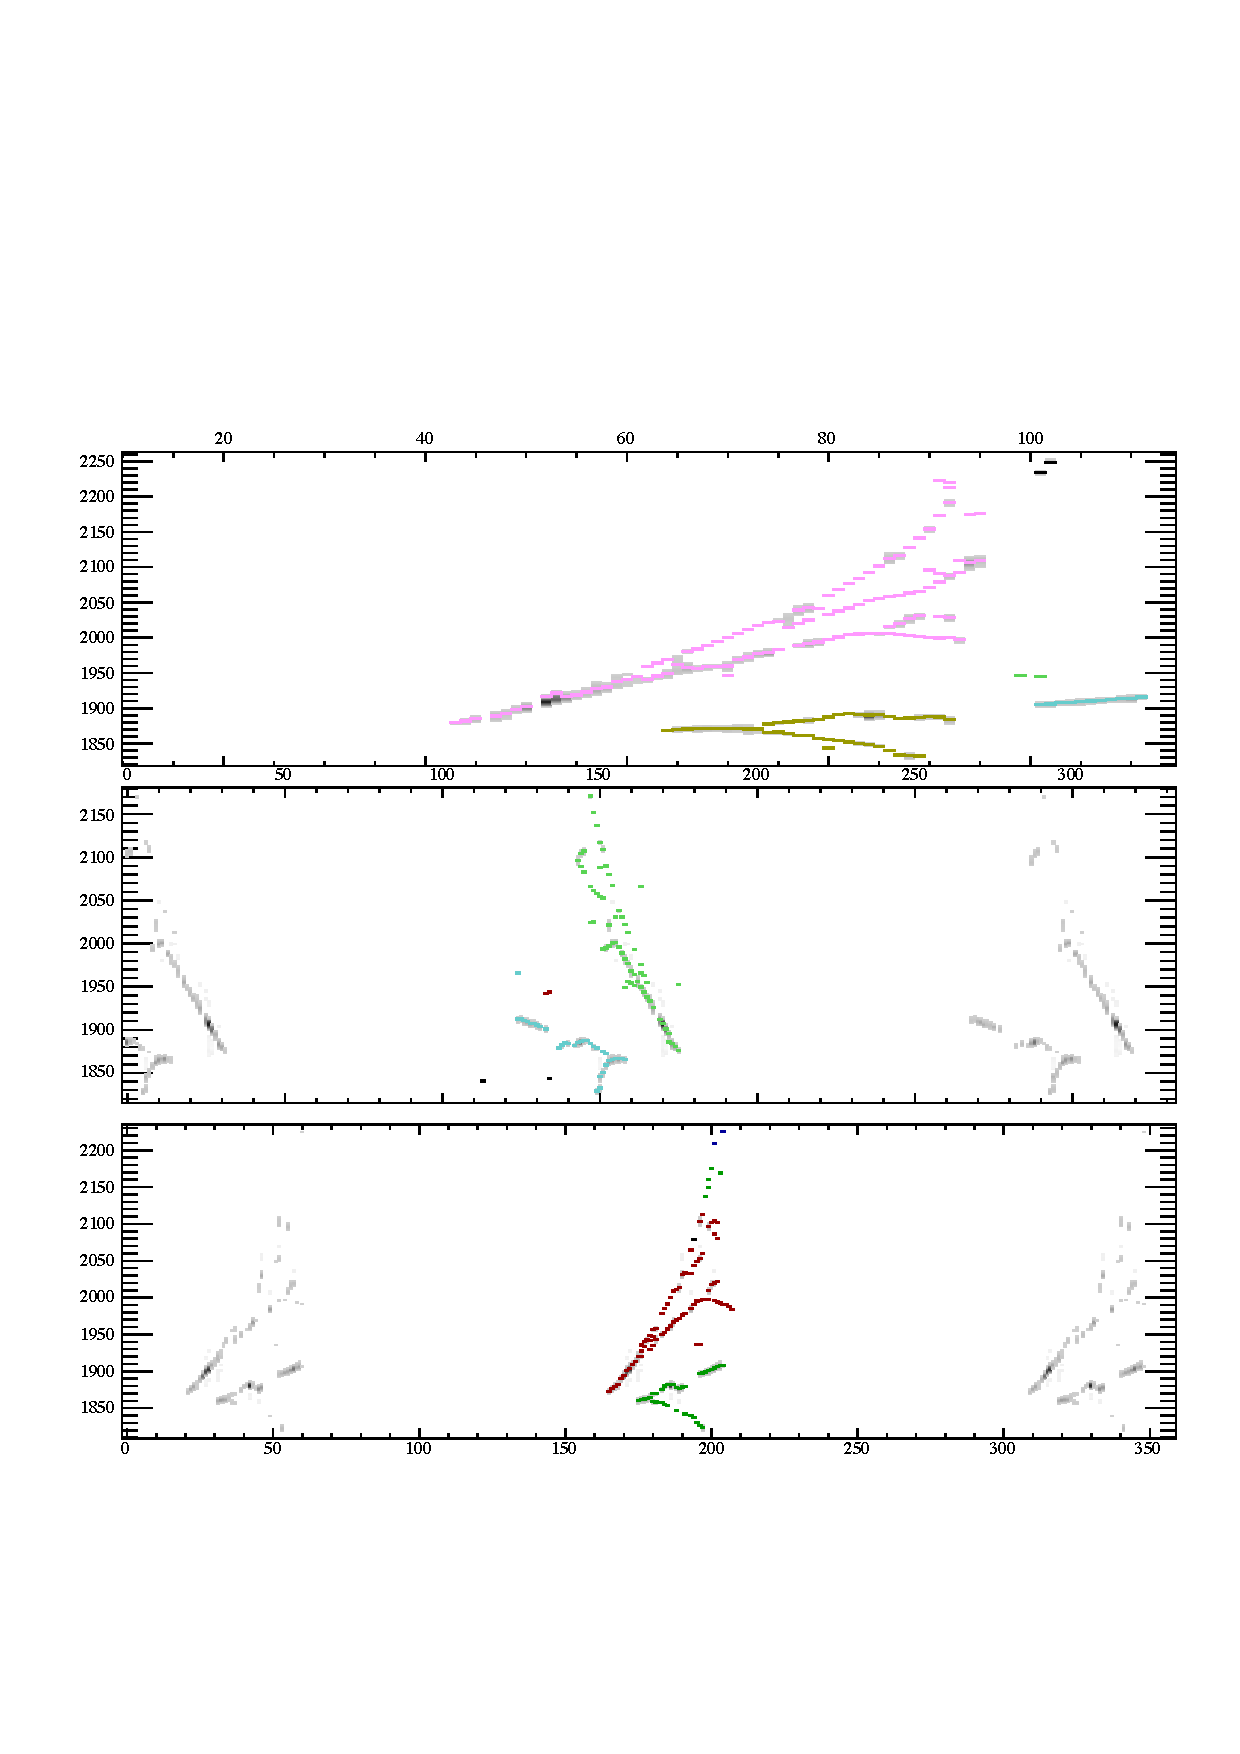
\includegraphics[width=10cm]{EVDPi0Clusters.pdf}
  \caption[The 2D clusters made using BlurredCluster when applied to the 35~ton $\pi^0$ event shown in Figure~\ref{fig:pi0Showers}.]{The 2D clusters made using BlurredCluster when applied to the 35~ton $\pi^0$ event shown in Figure~\ref{fig:pi0Showers}.  The different colours represent separate cluster objects.}
  \label{fig:pi0ShowersClusters}
\end{figure}

%----------------------------------------------------------------------------------------------------------------------------------------------------------------------------
\subsubsection{Configuring the Clustering}\label{sec:BlurredClusterConfiguration}

The BlurredCluster algorithm takes reconstructed hits as input, previously determined by a LArSoft hit finder (such as gaushit).  It places the output clusters, along with associations to the hits which comprise them, back into the event record.  There are multiple user-defined parameters which must be tuned to provide the best reconstruction.  This has been done for both the DUNE 35~ton and FD geometries and is dependent on detector properties such as the induction wire angle and anode wire pitch.

There are two ways in which the reconstruction can be performed in a given detector; either for each cryostat, drift volume (DV) and plane separately or alternatively across all DVs for each plane in a given cryostat.  This distinction is necessary due to the detector readout, which arbitrarily breaks up the active region into distinct DVs depending on the APA which reads the charge out.  When performing reconstruction, it is unnatural to consider each DV separately and so instead a `global' volume is defined.  Such a coordinate assigns a wire number for all wires on a given plane in a single cryostat, agnostic to the boundaries defined by the detector hardware.  This scheme is demonstrated in Figure~\ref{fig:GlobalWire} and is used by default by BlurredCluster.

\begin{figure}
  \centering
  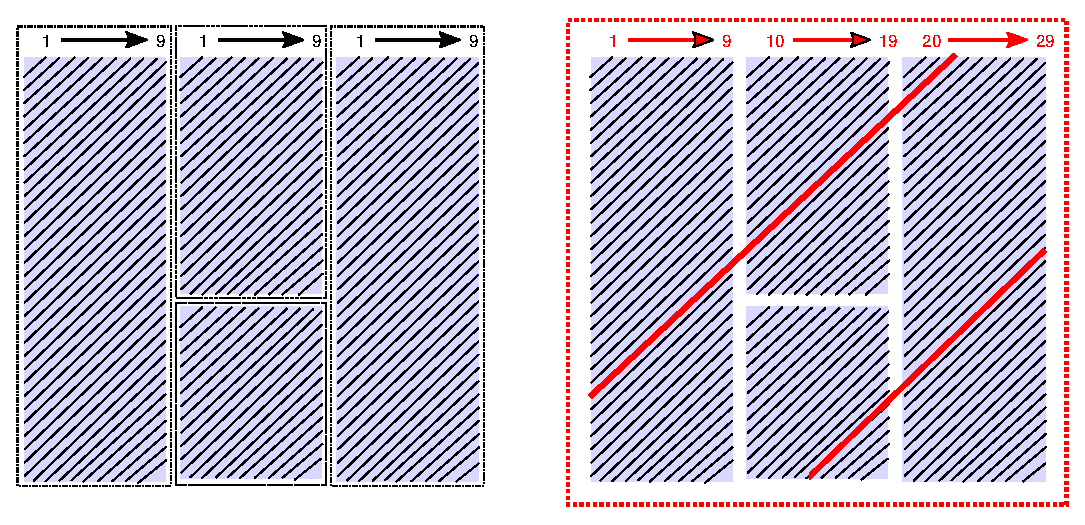
\includegraphics[width=12cm]{GlobalWire.eps}
  \caption[Demonstration of the `global wire' concept in single-phase LArTPC reconstruction.]{Demonstration of the `global wire' concept in single-phase LArTPC reconstruction.  A single hypothetical induction plane is shown across the 4~APAs in the 35~ton geometry.  The blue boxes represent the APAs and the black lines and numbering at the top show the wires in one plane.  In the left-hand figure, the APAs are considered separately and the conventional wire numbering is shown, with each wire represented by four numbers: the cryostat, DV, plane and wire number.  Reconstruction may be performed in each DV independently using the wire number as the spatial coordinate.  In the right-hand figure, the entire volume is considered as a whole and the wires are renumbered to reflect their position in the global geometry.  An imaginary line connecting wires which would overlap others on different APAs (and thus different DVs) if extended is used to give each of the wires a common index.  In this scheme, each is described using just three numbers: the cryostat, plane and global wire.}
  \label{fig:GlobalWire}
\end{figure}

%----------------------------------------------------------------------------------------------------------------------------------------------------------------------------
\subsection{EMShower Algorithm}\label{sec:EMShower}

The EMShower algorithm is a 3D shower reconstruction algorithm implemented within LArSoft \cite{EMShower,EMShowerLArSoft}.  It was conceived as an extension of the 2D BlurredCluster reconstruction method and takes these clusters as input.  The philosophy behind such a design choice is to perform as much of the reconstruction as possible in 2D, where most of the information exists, before simply applying a 3D matching algorithm to the output to produce complete objects.  Since BlurredCluster has been shown to produce very well formed, complete clusters, EMShower essentially just combines these clusters together to form 3D shower objects.

The shower reconstruction is intended to be very high-level and depend heavily on previous reconstruction to take advantage of as much available information as possible.  It is written very generically, making no assumptions on the specifics of the detector geometry such as the number of planes (LArIAT, which only possesses two readout planes, successfully uses EMShower to reconstruct showers).  The shower-forming proceeds in two general steps: pattern recognition provides the geometrical shower shapes by combining 2D clusters from multiple views before analysis of the hits across the views is performed to determine properties of these shower objects.  These stages will be discussed in the following Sections~\ref{sec:EMShowerPattern} and~\ref{sec:EMShowerProperties} respectively.

%----------------------------------------------------------------------------------------------------------------------------------------------------------------------------
\subsubsection{Shower Pattern Forming}\label{sec:EMShowerPattern}

Taking advantage of the well developed tools already within LArSoft, EMShower performs cluster matching by utilising previously conducted 3D track reconstruction.  This is demonstrated in Figure~\ref{fig:pi0ShowersTracks}, which shows the output of BlurredCluster adjacent to the 3D tracks found by the Projection Matching Algorithm for the 35~ton $\pi^0$ event shown in Figure~\ref{fig:pi0Showers}.  It is clear how using the respective hit associations facilitates connections between 2D clusters and 3D tracks, essentially matching the clusters between the views and forming 3D objects.  The output from this stage is a collection of hits which are assumed to be part of the same shower object; the shower properties are determined by analysing these hits.

\begin{figure}
  \centering
  \begin{subfigure}[t]{0.48\linewidth}
    \centering
    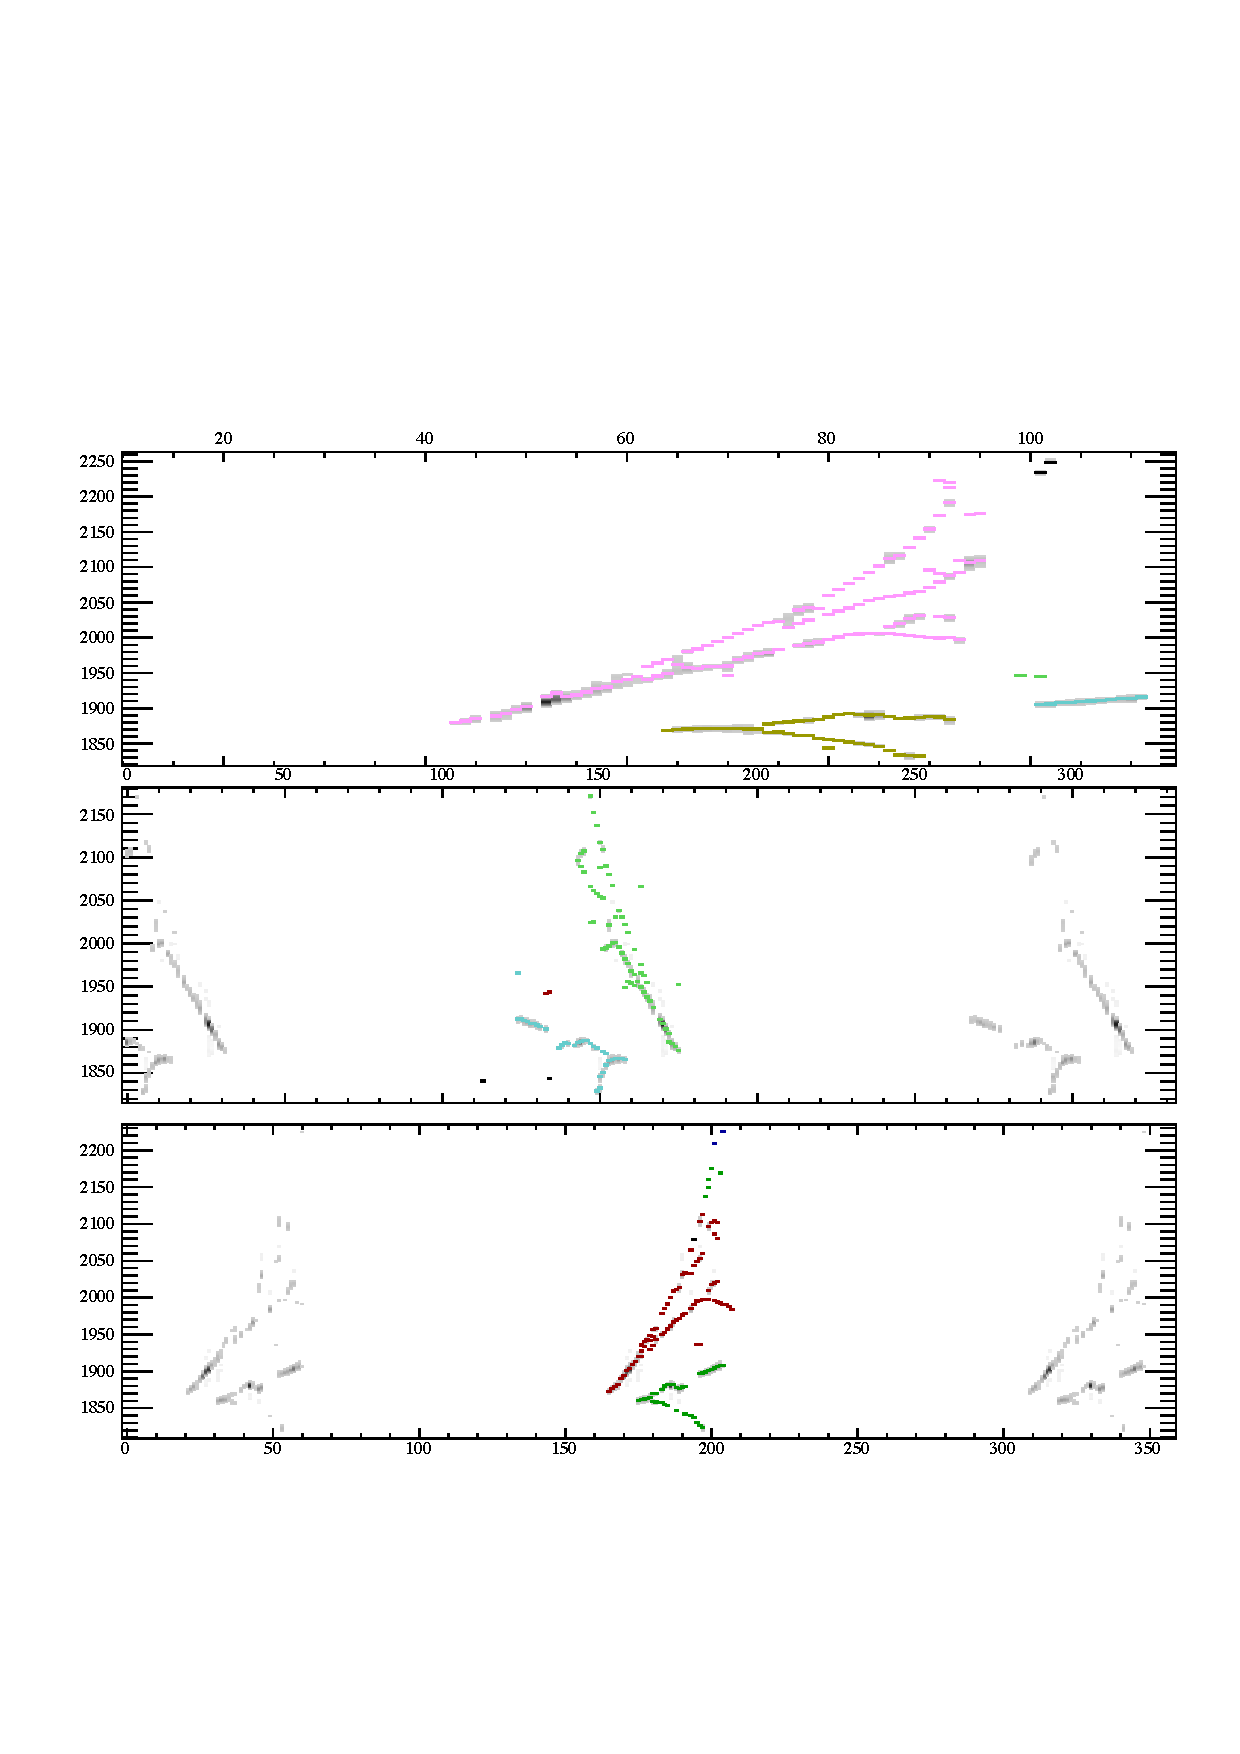
\includegraphics[width=0.98\textwidth]{EVDPi0Clusters.pdf}
    \caption{BlurredCluster.}
    \label{fig:pi0ShowersTracksClusters}
  \end{subfigure}
  \hfill
  \begin{subfigure}[t]{0.48\linewidth}
    \centering
    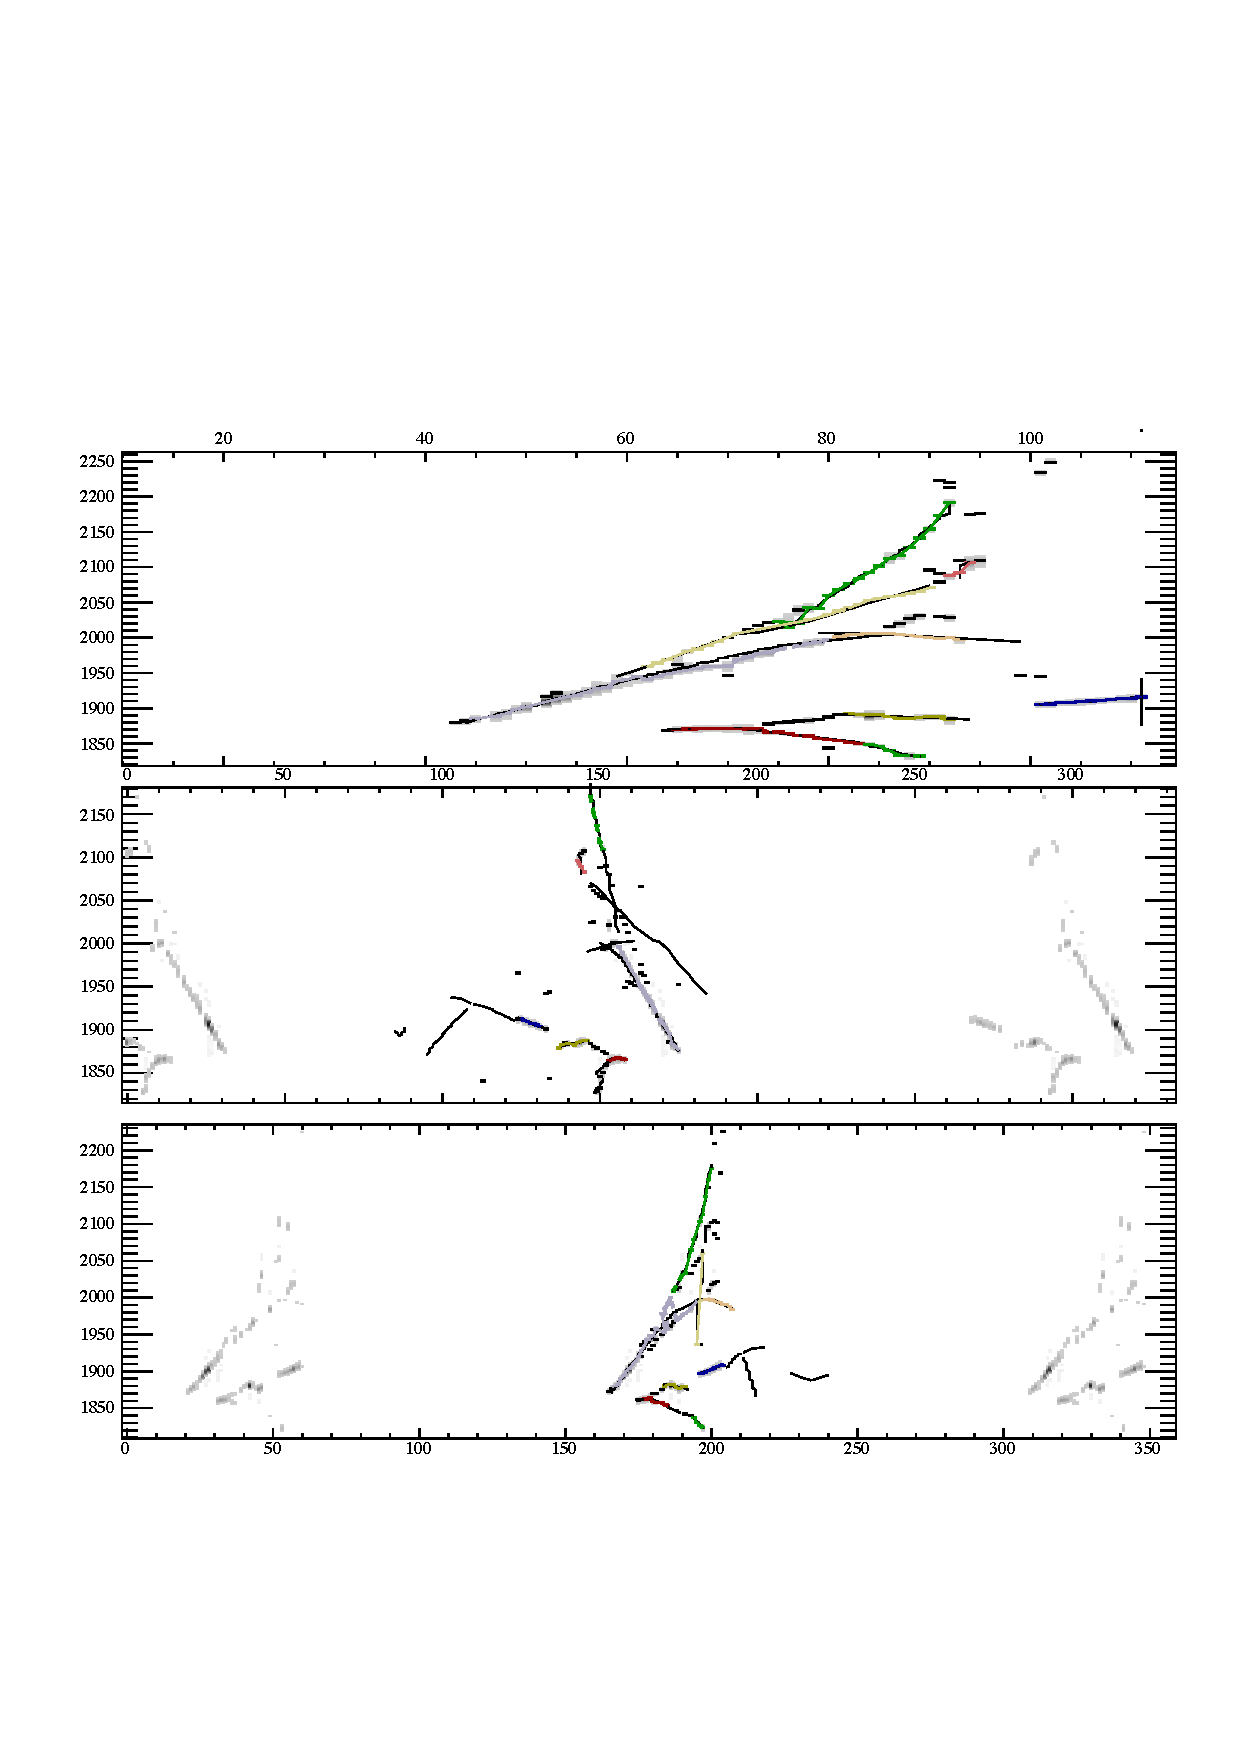
\includegraphics[width=0.98\textwidth]{EVDPi0Tracks2D.pdf}
    \caption{Projection Matching Algorithm.}
    \label{fig:pi0ShowersTracksTracks}
  \end{subfigure}
  \caption[Comparison of the 2D shower cluster reconstruction and the 3D tracking reconstruction for a 35~ton $\pi^0$ event.]{Comparison of the 2D shower cluster reconstruction and the 3D tracking reconstruction for a 35~ton $\pi^0$ event.  In both cases, the different colour represent individually reconstructed objects.  It should be noted that, due to the 3D nature of the tracks, the same colours are evident across multiple views in Figure~\ref{fig:pi0ShowersTracksTracks}, representing the hits used to construct the shower in each plane.}
  \label{fig:pi0ShowersTracks}
\end{figure}

The algorithm performs checks to ensure two cluster merge candidates are indeed related to the same particle.  The number of track hits associating the clusters and the length of the track are taken into account before matching two objects across views.  Additionally, with three planes, it is possible to analyse the 2D reconstruction to determine, for example, whether or not one plane contains one large cluster whilst the other two planes contain two smaller clusters, which may be indicative of poor reconstruction in the first view.

%----------------------------------------------------------------------------------------------------------------------------------------------------------------------------
\subsubsection{Shower Properties Reconstruction}\label{sec:EMShowerProperties}

Following the formation of the showers and the identification of all the associated hits in each view, the properties of the object may be determined.  The shower energy may be determined for each plane using the method discussed in Section~\ref{sec:ShowerEnergy}.  For all other relevant properties, it is imperative the start of the shower is successfully found and efficiently reconstructed.  From this initial track before the particle begins to shower, the start point (conversion point), initial direction and dE/dx may be determined.

In order to orient the shower, the hits are analysed in each plane separately whilst using information from other planes to validate.  Initially, the hits in each plane are assembled into a rough `order', corresponding to how far along the shower each is.  This is achieved by projecting each hit onto the axis determined using a least squares fit on all the hits in a given view.  In most cases, this order is accurate but not necessarily oriented correctly.  Occasionally, if the shower is not very well formed (such as if it travels very parallel to the wires) in one plane, the hit order is not defined and the view is discarded for the purposes of shower start finding.  This is accomplished by comparing the RMS of the perpendicular distance of all hits from the central axis and removing views in which this differs significantly.

Once there is sufficient confidence that the hits are correctly ordered in the remaining planes, they are then oriented correctly.  This is done by evaluating the `RMS gradient', the RMS of the distribution of the hits in discrete segments along the length of the shower.  Figure~\ref{fig:EMShowerOrientation} demonstrates how this may be utilised to correctly orient the shower.  This represents an overly simplified case but this method has been found to work surprisingly well across a wide range of differing shower and event topologies, at least as an initial guess.  Additional checks are in place to ensure the orientations agree between views and to reevaluate the shower ordering if necessary.

\begin{figure}
  \centering
  \begin{subfigure}[t]{0.48\linewidth}
    \centering
    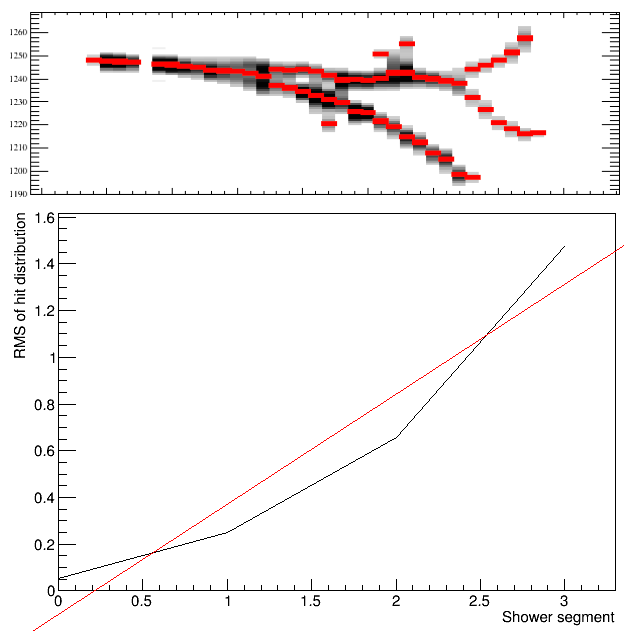
\includegraphics[width=0.98\textwidth]{ShowerReconDirectionPositive.png}
    \caption{Positive gradient.}
    \label{fig:EMShowerOrientationPositive}
  \end{subfigure}
  \hfill
  \begin{subfigure}[t]{0.48\linewidth}
    \centering
    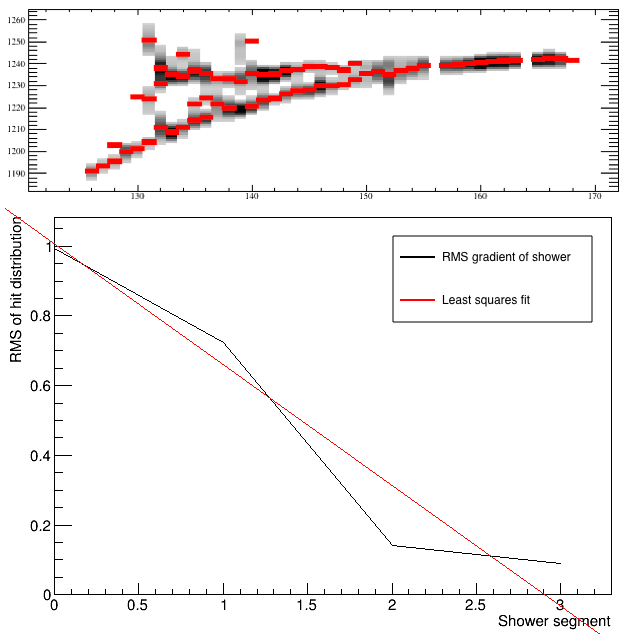
\includegraphics[width=0.98\linewidth]{ShowerReconDirectionNegative.png}
    \caption{Negative gradient.}
    \label{fig:EMShowerOrientationNegative}
  \end{subfigure}
  \caption[Demonstration of the method utilised to ensure a correct shower orientation of the shower in a given view for the purpose of shower start finding in the EMShower algorithm.]{Demonstration of the method utilised to ensure a correct shower orientation of the shower in a given view for the purpose of shower start finding in the EMShower algorithm.}
  \label{fig:EMShowerOrientation}
\end{figure}

After correctly orientating the hits along the axis of the shower in each view separately, it is straight forward to determine the initial track-like parts.  For each plane, the hits are considered in order until it becomes obvious the shower is diverging (e.g. multiplicity of hits on the wires).  The initial shower hits from each of the planes are combined in order to construct a 3D track object, which is used to provide a start point and direction.  These hits are additionally analysed to provide a dE/dx for the start of the shower.

The result of applying the full EMShower algorithm to the 35~ton $\pi^0$ event from Figure~\ref{fig:pi0Showers} is presented in Figure~\ref{fig:pi0ShowersShowers}.  The complete 3D shower objects for each photon are evident with well reconstructed properties, demonstrating the successful shower reconstruction provided by BlurredCluster and EMShower together.  The reconstruction is characterised and validated further in Section~\ref{sec:ReconstructionPerformance}.

\begin{figure}
  \centering
  \begin{subfigure}[t]{0.48\linewidth}
    \centering
    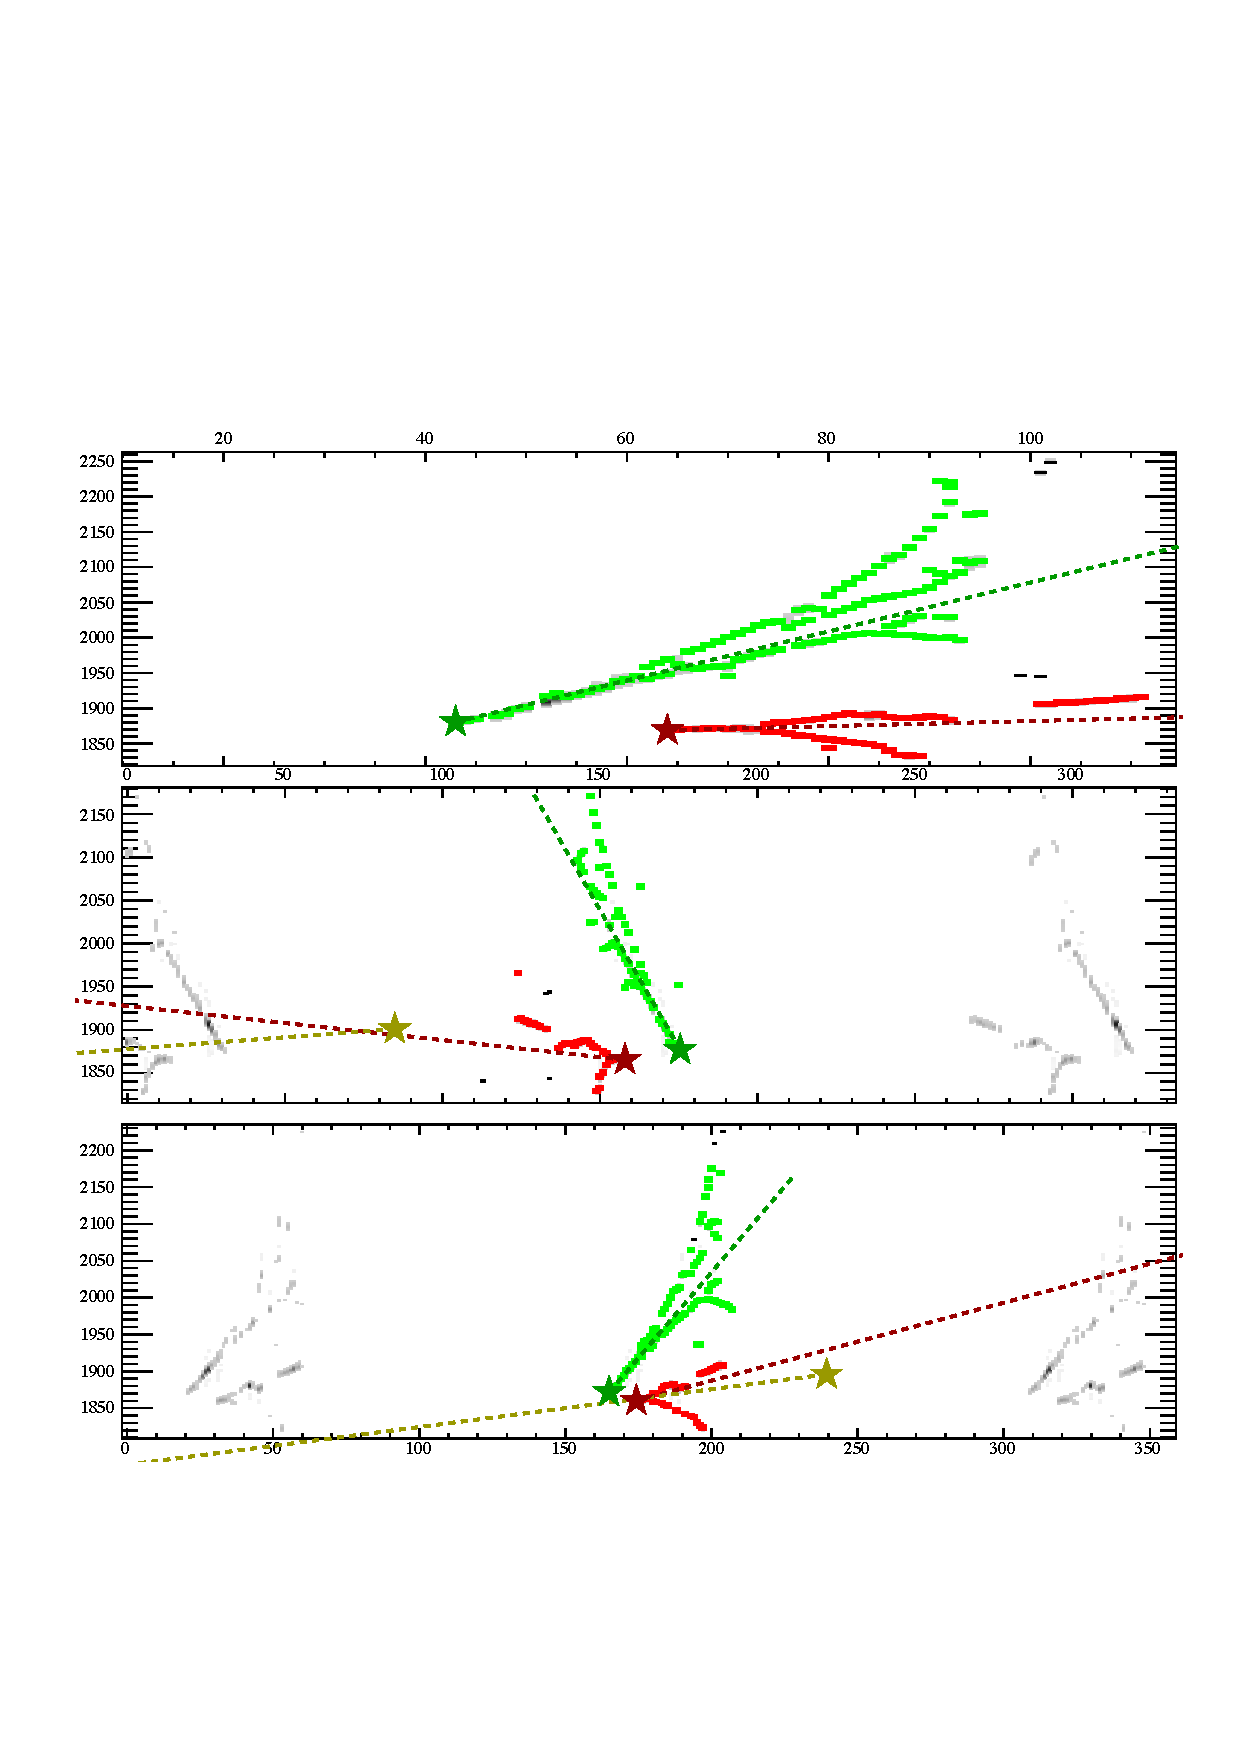
\includegraphics[width=0.98\textwidth]{EVDPi0Shower2D.pdf}
    \caption{2D.}
    \label{fig:pi0ShowersShowers2D}
  \end{subfigure}
  \hfill
  \begin{subfigure}[t]{0.48\linewidth}
    \centering
    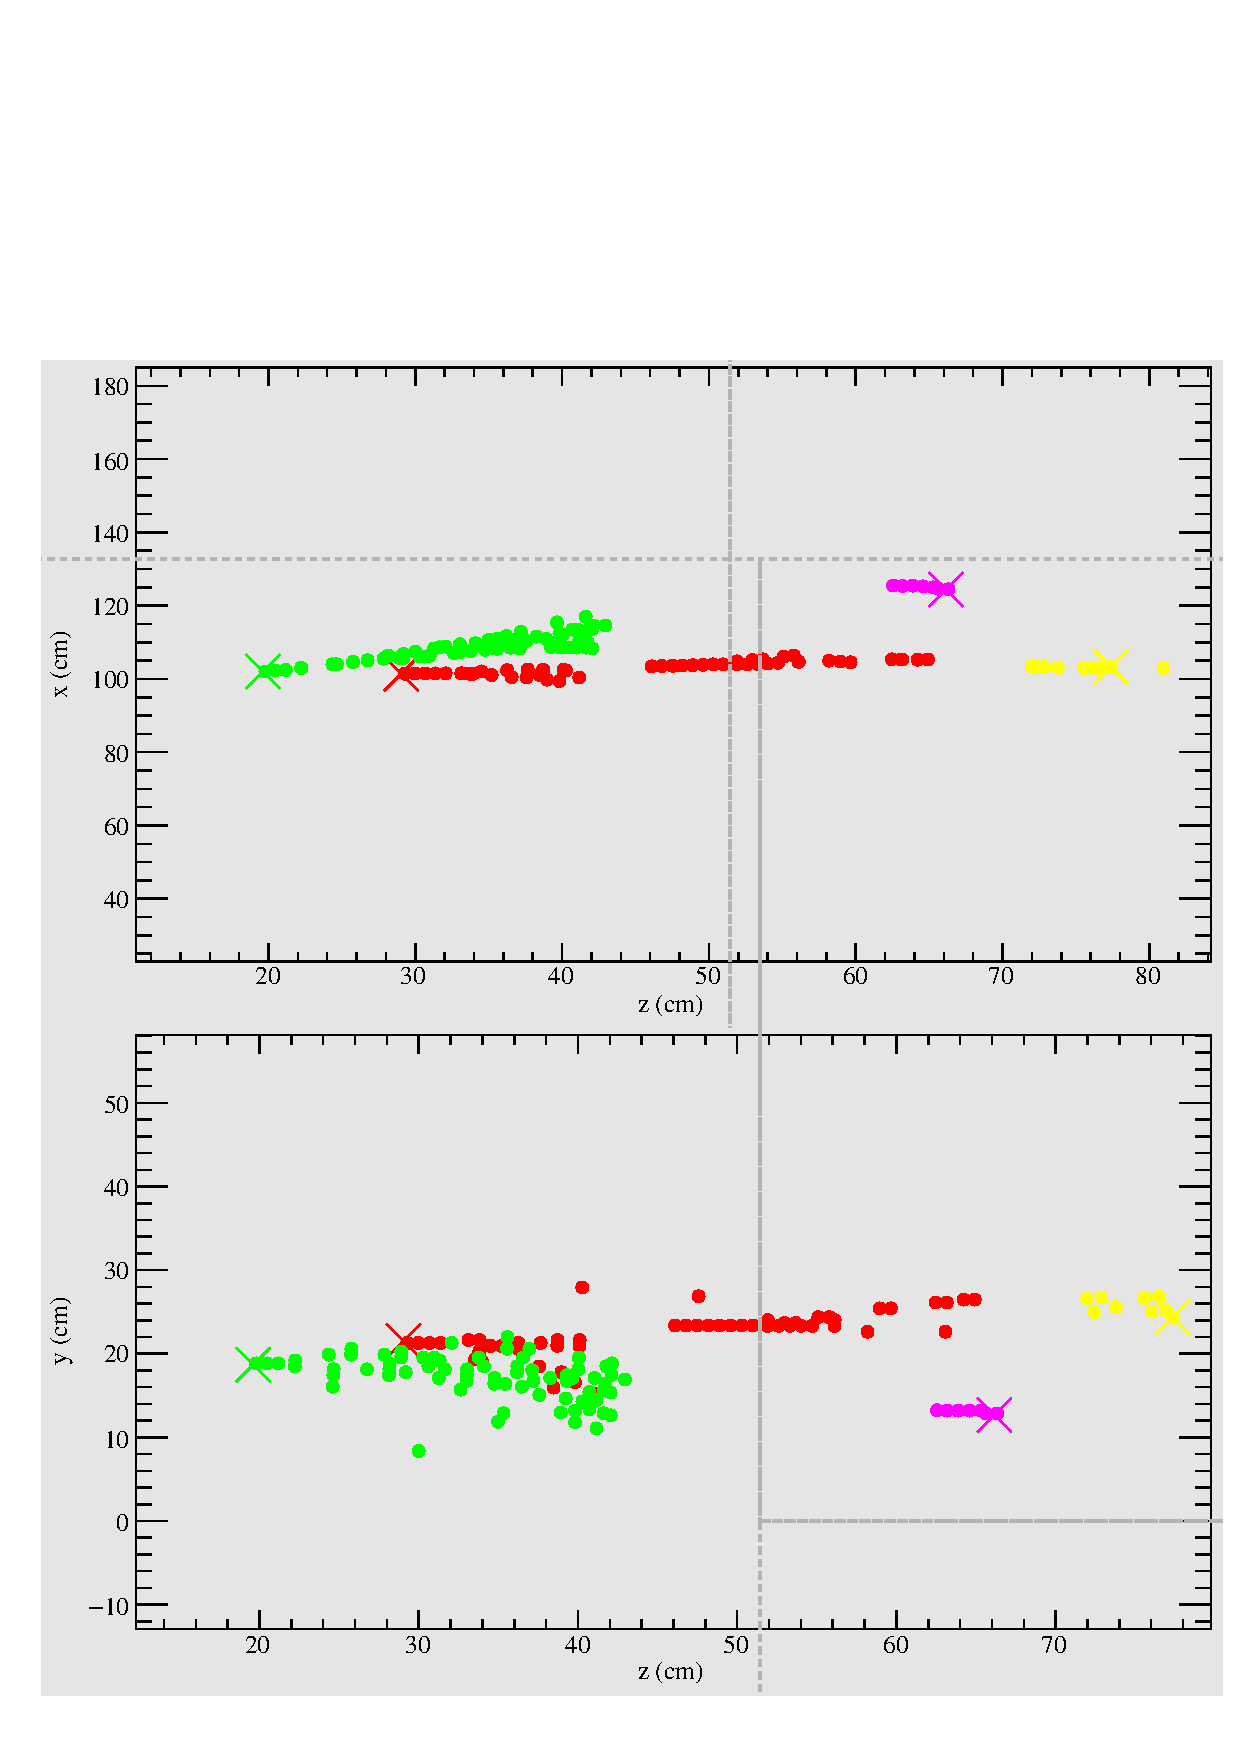
\includegraphics[width=0.98\textwidth]{EVDPi0Shower3D.pdf}
    \caption{3D.}
    \label{fig:pi0ShowersShowers3D}
  \end{subfigure}
  \caption[The output from the full 3D shower reconstruction provided by BlurredCluster/EMShower when applied to the 35~ton $\pi^0$ event shown in Figure~\ref{fig:pi0Showers}.]{The output from the full 3D shower reconstruction provided by BlurredCluster/EMShower when applied to the 35~ton $\pi^0$ event shown in Figure~\ref{fig:pi0Showers}.  The showers are shown in both the 2D wire/tick view in Figure~\ref{fig:pi0ShowersShowers2D} and in the orthogonal 3D representation in Figure~\ref{fig:pi0ShowersShowers3D}.  The stars/crosses represent the reconstructed start point and the dotted lines the reconstructed direction.}
  \label{fig:pi0ShowersShowers}
\end{figure}

%----------------------------------------------------------------------------------------------------------------------------------------------------------------------------
\subsection{Track/Shower Separation}\label{sec:TrackShowerSeparation}

The shower reconstruction described in Sections~\ref{sec:BlurredCluster} and~\ref{sec:EMShower} is optimised for shower-like hits and makes no attempt to ignore hits which originate from tracks.  This issue of track/shower separation is a hugely complex problem in LArTPCs and remains largely unsolved.  Significant progress has been made in the last year however, mainly via the use of machine learning.  The vastly differing topologies, wide band energies in the DUNE beam and highly detailed event information all contribute to a challenging reconstruction issue unlikely to be solved without the use of deep learning algorithms.

This section briefly details the development of an alternative approach to the problem, which was found to be inferior to the more recent developments.  It is nonetheless instructive to overview the subject and assess the attempted method to evaluate how the experience may inform other potential strategies in addressing the issue.

The algorithm was developed primarily for the purposes of the $\nu_e$CC oscillation appearance selection, the subject of Chapter~\ref{chap:FDAnalysis}.  An example $\nu_e$CC event is demonstrated in Figure~\ref{fig:nueCC}.  The topologies of the different particle objects are evident by eye and the purpose of the track/shower separation is to remove the track-like hits from the events, leaving just shower-like hits over which the shower reconstruction algorithms may be run.

\begin{figure}
  \centering
  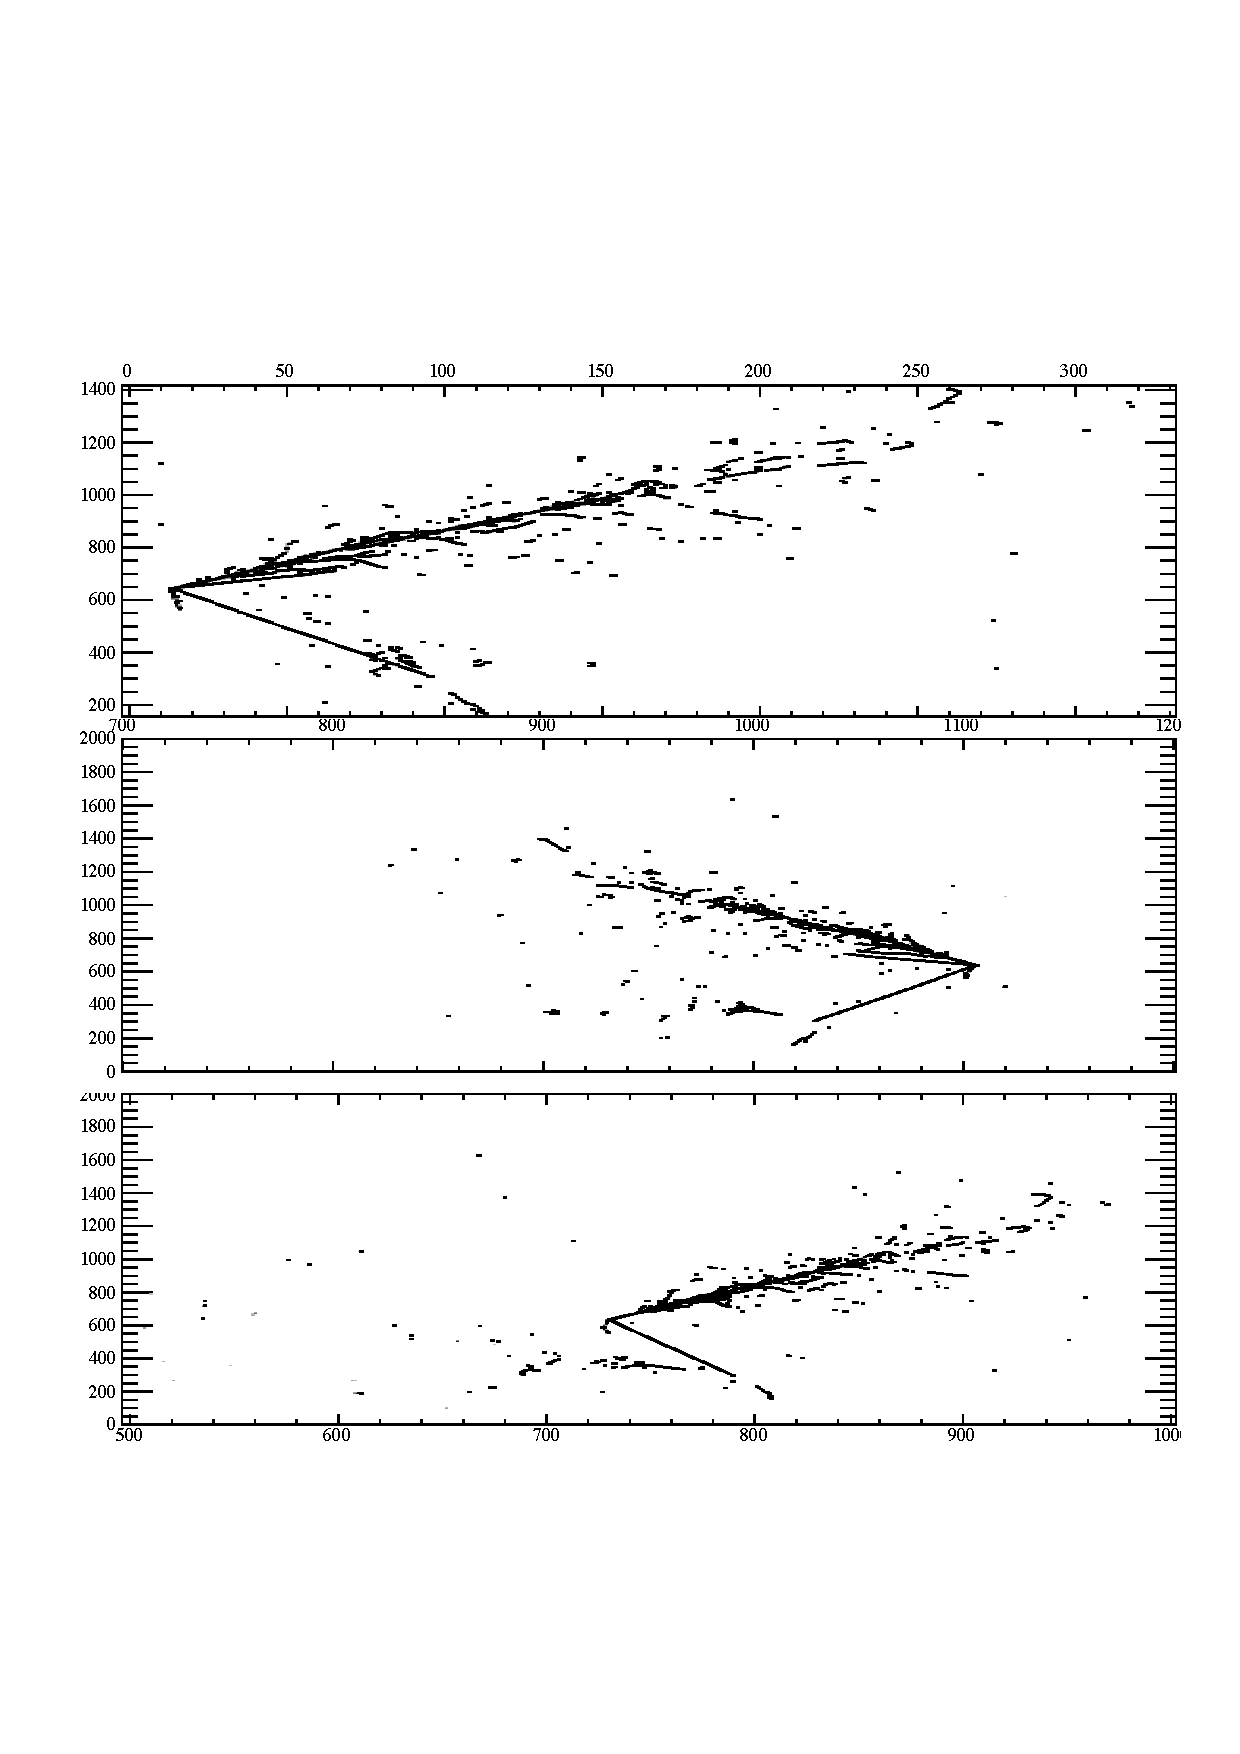
\includegraphics[width=10cm]{NuECCHits.pdf}
  \caption[An example $\nu_e$CC interaction in the DUNE far detector.]{An example $\nu_e$CC interaction in the DUNE far detector.  The Gaussian hit finder has been used to reconstruct hits, shown as black rectangles.  The electron shower is evident, along with many other smaller hadron tracks.  The $\nu_e$ energy in this event is 3.7~GeV and the electron has an energy of 1.9~GeV.}
  \label{fig:nueCC}
\end{figure}

Following the success of EMShower, which utilised as much previously executed reconstruction as possible to access all available information about an event, the track/shower separation was also conceived to benefit in this way.  It is designed to be performed following track finding and, in essence, simply analyses each of the reconstructed track objects to identify which are the result of track-like particles.  The associated hits are then removed from the sample passed on to BlurredCluster for shower reconstruction.

A typical, though simplified, event, containing a track and shower, is demonstrated in Figure~\ref{fig:TrackShowerTopology}.  The three topological objects are noted as a \textit{track}, a \textit{shower track} (the initial part of a shower before the electromagnetic cascade occurs) and a \textit{shower cone} (the rest of the shower downstream of the shower track).  The track/shower separation treats each of these objects independently to ensure a complete evaluation of the entire topology.  The algorithm proceeds in the following general steps:
\begin{itemize}
  \item tracks-like objects (including \textit{tracks} and \textit{shower tracks}) are identified;
  \item \textit{shower tracks} are identified;
  \item \textit{shower cone} activity is identified.
\end{itemize}

\begin{figure}
  \centering
  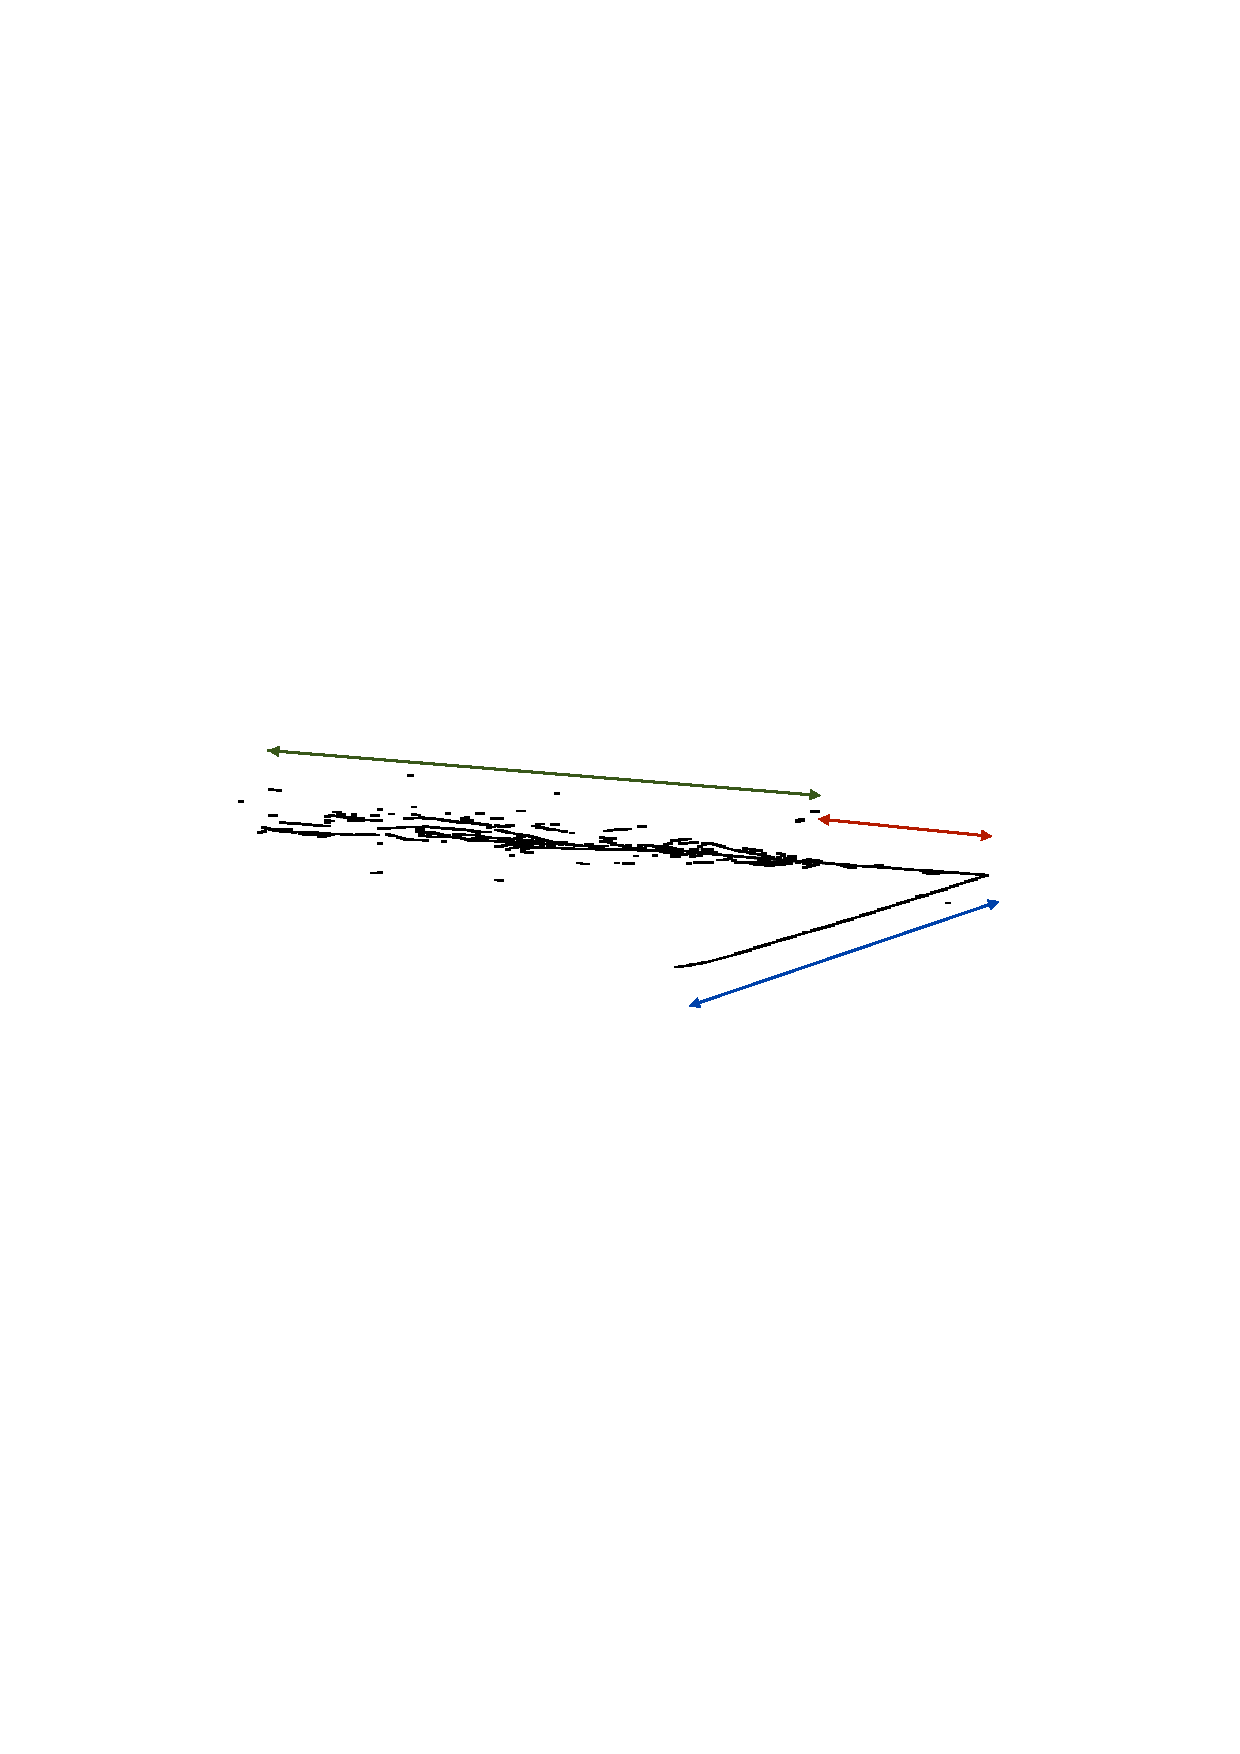
\includegraphics[width=12cm]{TrackShowerExampleEVDAnnotated.pdf}
  \caption[A simplified event topology demonstrated typical track and shower topologies.]{A simplified event topology demonstrated typical track and shower topologies.  The three distinct features are highlighted; the blue label represents a track, the red a `shower track' and the green a `shower cone'.}
  \label{fig:TrackShowerTopology}
\end{figure}

The \textit{tracks} and \textit{shower tracks} are deduced by considering additional activity along the length of each previously reconstructed track object, in both 2D and 3D.  Tracks which do not belong to the shower cone have a characteristically lower amount of external hits in a surrounding cylinder or rectangle, and are identified with good efficiency.  Following this, the number of previously determined tracks and hits in a projection from either end of these track-like objects may be used to distinguish \textit{shower tracks}.  The \textit{shower cones} are determined by examining the event following the determination of any \textit{shower tracks}.  Additional checks are in place, such as reevaluating a track-like object upon discovering a large amount of activity downstream of its end and reversing the orientation of objects based on other identified activity in the event, to ensure the method is as robust as possible.

The result of applying the algorithm to the DUNE $\nu_e$CC event shown in Figure~\ref{fig:nueCC} is demonstrated in Figure~\ref{fig:nueCCRecon}.  The electron shower is observed to be well separated from the other tracks from the vertex and reconstructed nicely.  This is a very successful reconstruction of the original event and may be utilised in the $\nu_e$CC selection discussed in Chapter~\ref{chap:FDAnalysis}.  A more general analysis of the performance of the reconstruction is considered in Section~\ref{sec:ReconstructionPerformance}.

\begin{figure}
  \centering
  \begin{subfigure}[t]{0.48\linewidth}
    \centering
    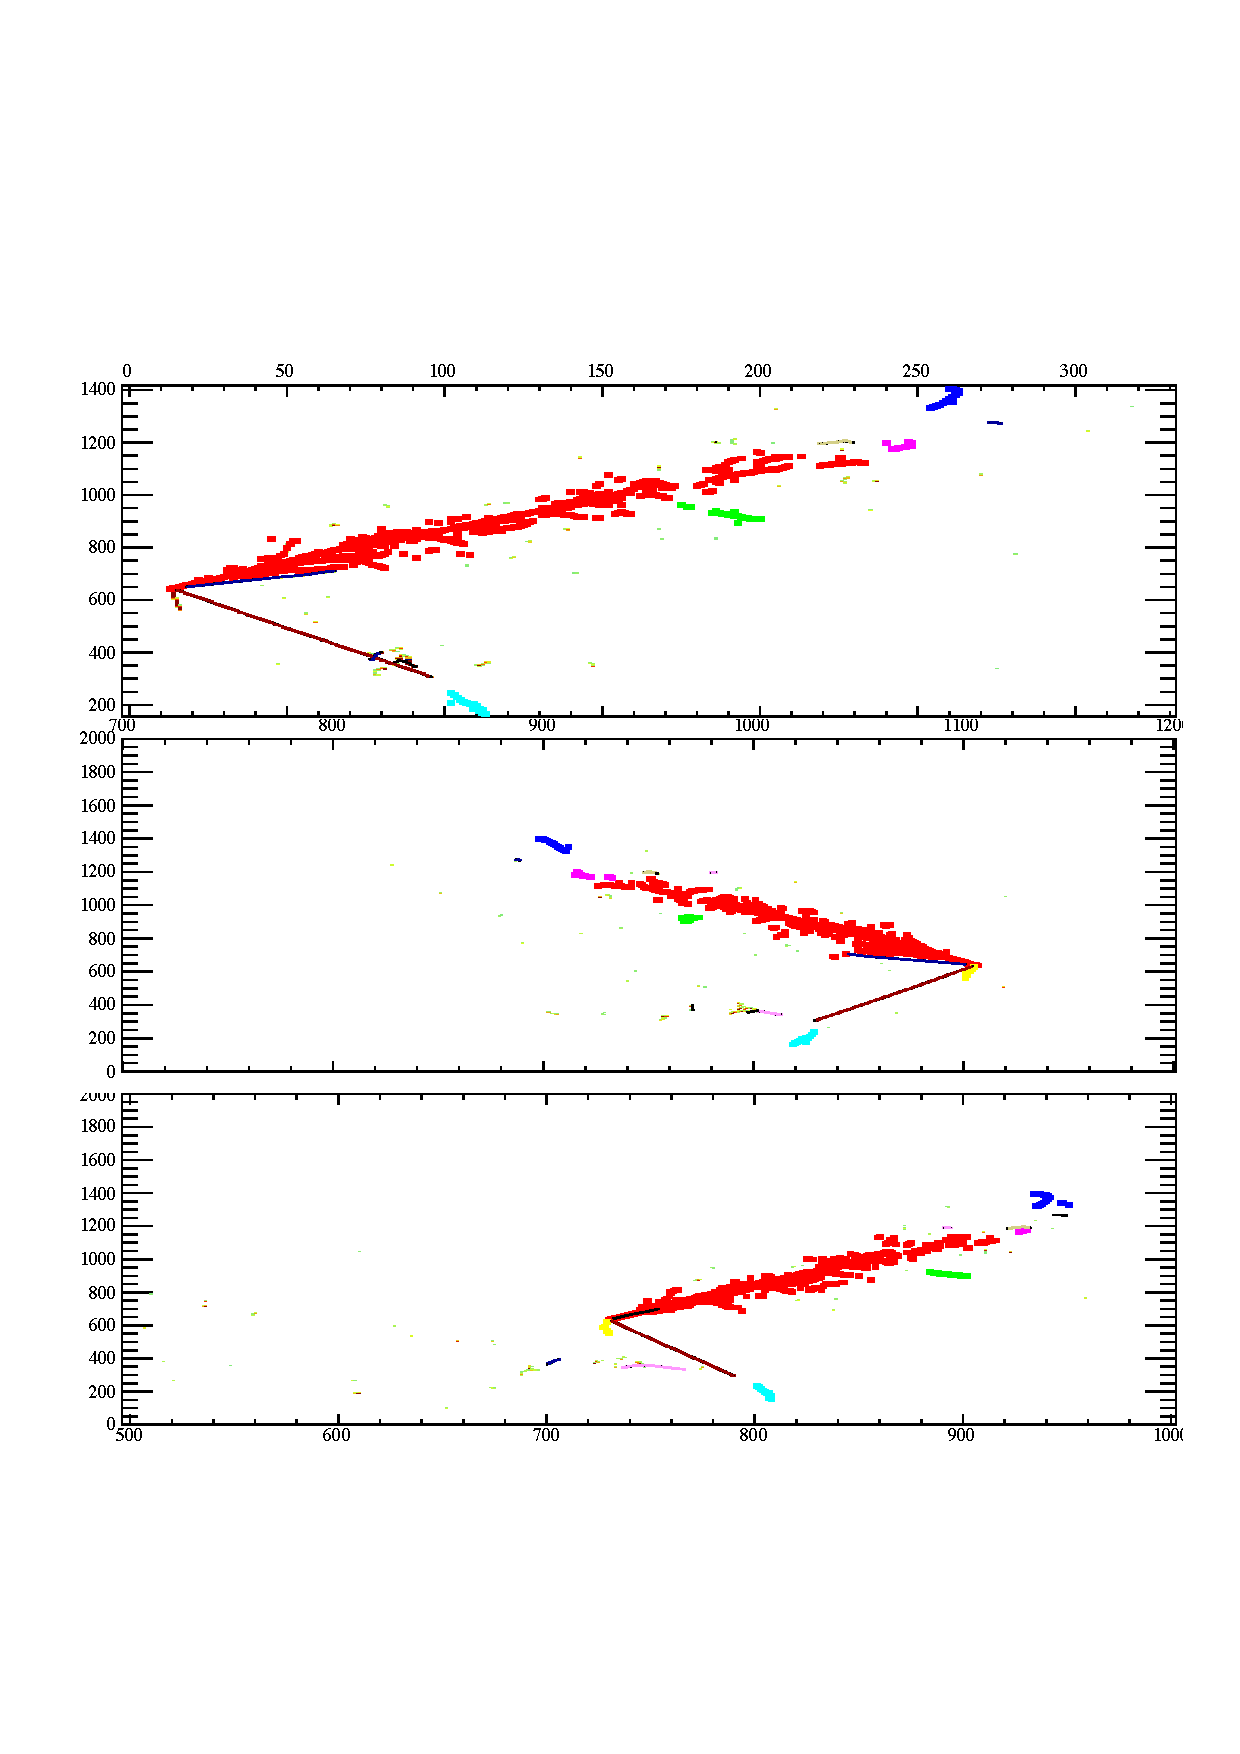
\includegraphics[width=0.98\textwidth]{NuECCTrackShower2D.pdf}
    \caption{2D.}
    \label{fig:nueCCRecon2D}
  \end{subfigure}
  \hfill
  \begin{subfigure}[t]{0.48\linewidth}
    \centering
    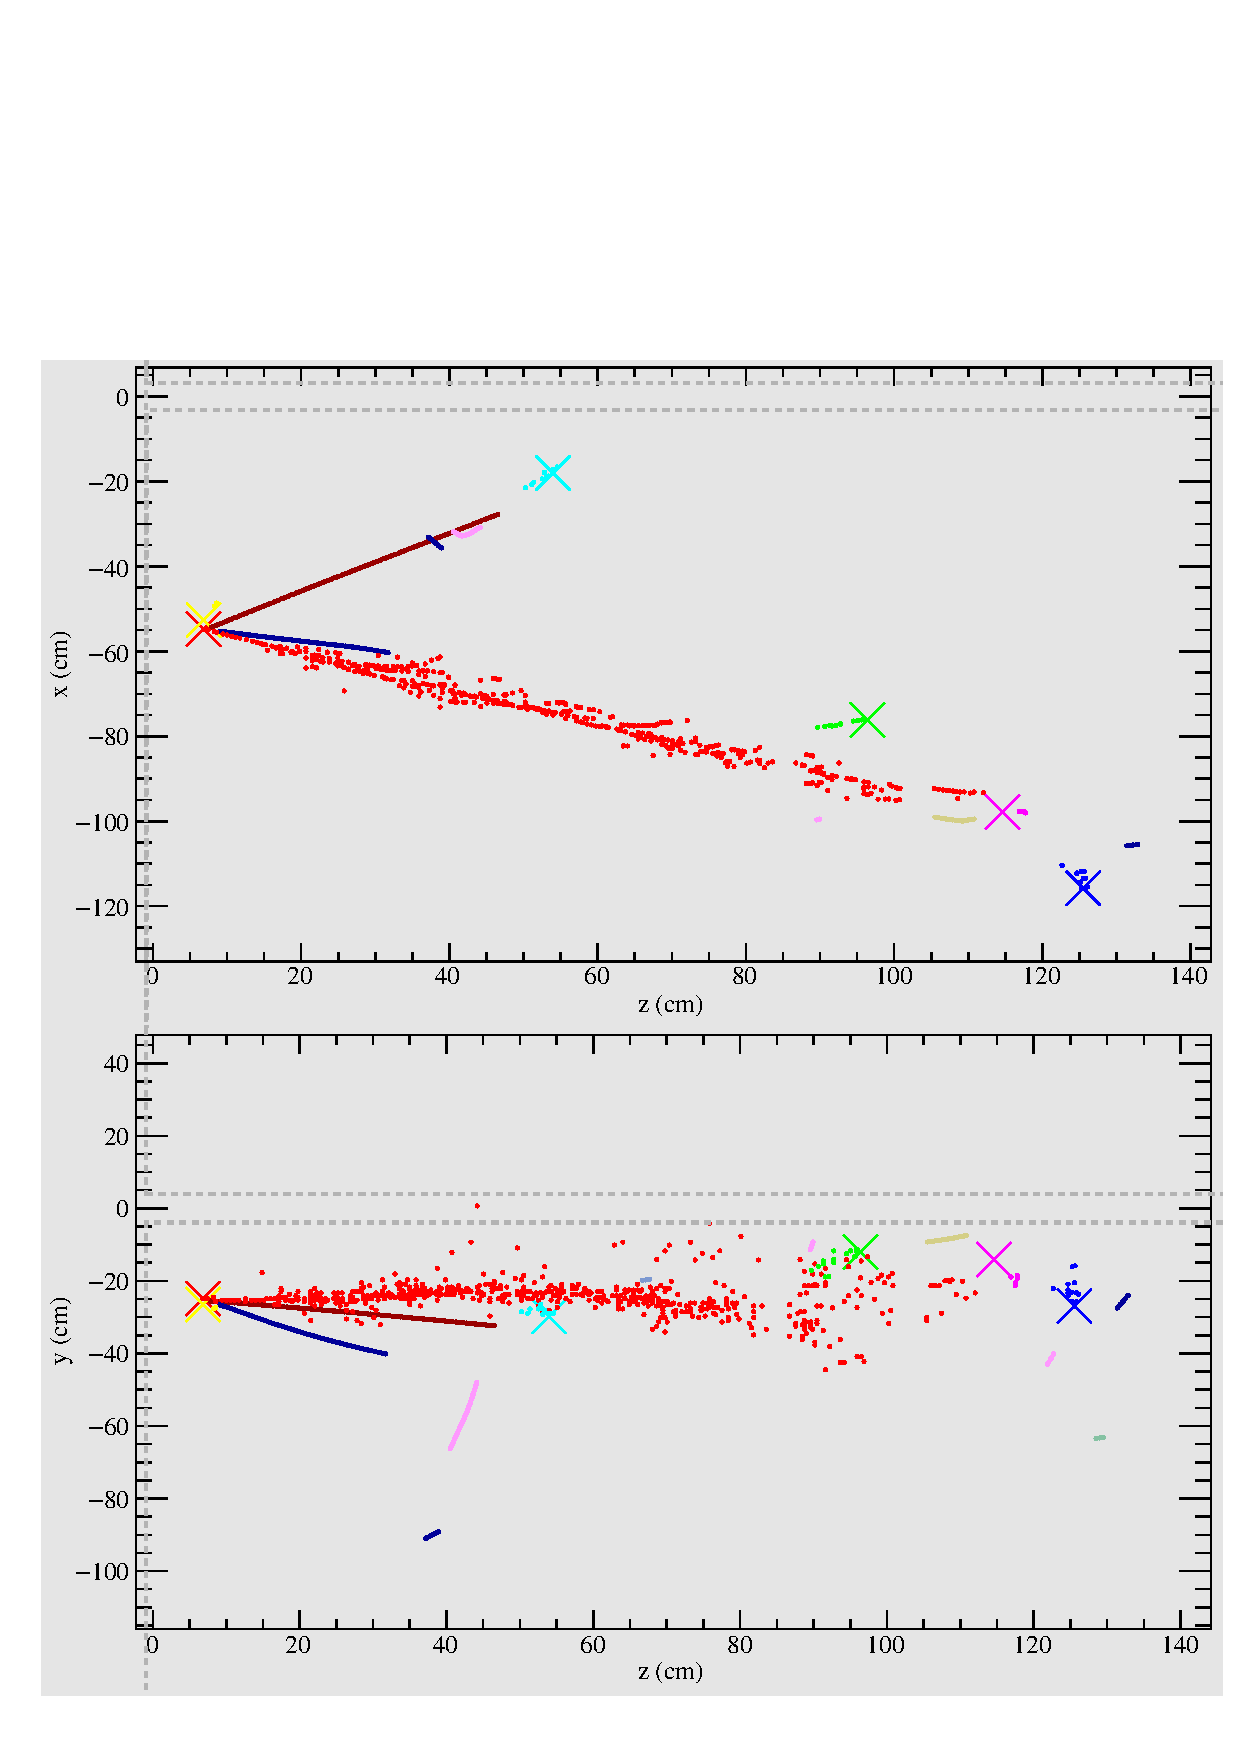
\includegraphics[width=0.98\textwidth]{NuECCTrackShower3D.pdf}
    \caption{3D.}
    \label{fig:nueCCRecon3D}
  \end{subfigure}
  \caption[The result of applying the track/shower separation, BlurredCluster and EMShower algorithms to the example DUNE far detector $\nu_e$CC event demonstrated in Figure~\ref{fig:nueCC}.]{The result of applying the track/shower separation, BlurredCluster and EMShower algorithms to the example DUNE far detector $\nu_e$CC event demonstrated in Figure~\ref{fig:nueCC}.  Both the 2D view and 3D projection are shown.}
  \label{fig:nueCCRecon}
\end{figure}

The reasoning behind performing this separation following the completion of track finding, as mentioned previously, is to utilise as much information as possible about the interaction.  There are however many drawbacks which were identified whilst developing the algorithm.  For example, any mistakes in the track reconstruction has implications on the success of the overall analysis of the event and may be a considerable problem.  Additionally, track reconstruction is not optimised in the important region around the vertex and often fails to distinguish separate particles or approaches a sensitive hit distribution too forcibly.  If the \textit{shower track} is not well reconstructed, or even just some hits misidentified, the method detailed above will often fail.  It became clear during the building of the framework that the track reconstruction would also hugely benefit from prior separation of hits, and that this problem must be solved at the hit, or even charge, level.  Such fine scrutiny is exceptionally challenging and it was only when utilising machine learning tools that the issue appeared resolvable.  As noted earlier, this is likely how the eventual solution will be found.

%----------------------------------------------------------------------------------------------------------------------------------------------------------------------------
\subsection{Performance of the Reconstruction}\label{sec:ReconstructionPerformance}

The performance of the reconstruction will be discussed in this section, with shower properties compared with true values (from the simulation) and with expectations.  The validation sample includes the following particles (generated using a particle gun with no other event activity):
\begin{itemize}
  \item Electrons, 0.1--5.0~GeV, 10~000 events, DUNE reduced far detector (10kt) geometry;
  \item Photons, 0.1--2.0~GeV, 10~000 events, DUNE reduced far detector (10kt) geometry;
  \item $\pi^0$s, 0.4--1.0~GeV, 10~000 events, DUNE 35~ton geometry.
\end{itemize}
The same, standard reconstruction was applied to each sample and the resulting shower objects analysed to quantify its functionality.

%----------------------------------------------------------------------------------------------------------------------------------------------------------------------------
\subsubsection{Shower Properties}\label{sec:ShowerProperties}

The efficacy in creating complete shower objects, including a reconstructed start point, direction, dE/dx, energy and associated hits, is demonstrated in Figure~\ref{fig:ShowerReconstructedEnergy}.  It is clear the reconstructed performs excellently at all energies above the very lowest, where the least amount of information is available to the reconstruction.  This is a very important feature of the reconstruction and great care was taken to ensure the reconstruction operates as effectively as possible.  It should be noted that this is only for single particle events, and less reliable reconstruction should be expected when the detector contains multiple particles, but it is nonetheless important in demonstrating basic capabilities.

\begin{figure}
  \centering
  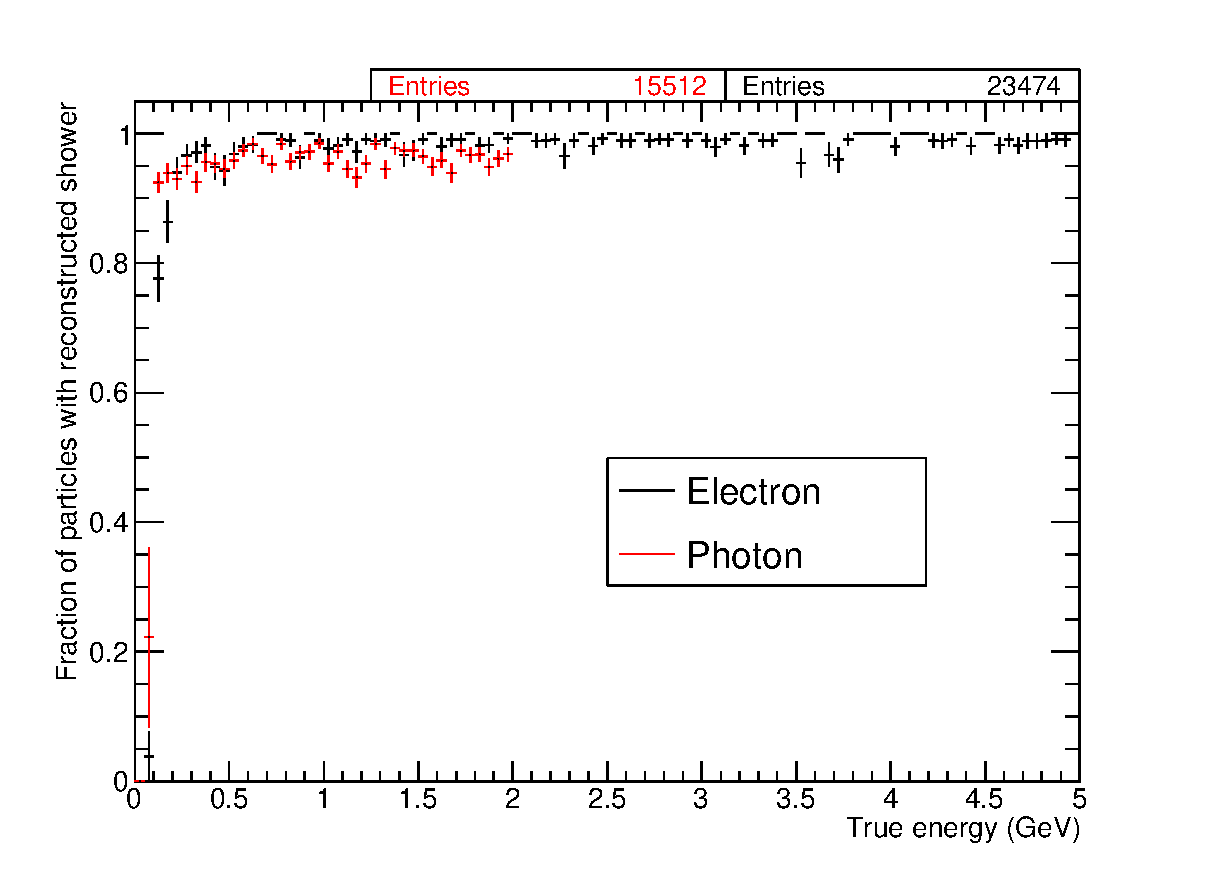
\includegraphics[width=10cm]{ShowerReconstructedEnergy.eps}
  \caption[The fraction of total shower particles for which a shower object is created when using BlurredCluster/EMShower reconstruction.]{The fraction of total shower particles for which a shower object is created when using BlurredCluster/EMShower reconstruction.  A complete reconstructed shower object is required to have a reconstructed start point, direction, dE/dx, energy and associated hits.}
  \label{fig:ShowerReconstructedEnergy}
\end{figure}

The quality of the reconstructed shower start point and direction is demonstrated in Figures~\ref{fig:ShowerStart} and~\ref{fig:ShowerDirection} respectively.  In both cases, it is clear in general the reconstruction performs very well at identifying the shower conversion point and extracting the relevant parameters.  The small (arguably insignificant) spike around zero in the direction plots results from challenging shower topologies in which a start point is successfully found but there is insufficient information from multiple planes to make an accurate direction measurement.

\begin{figure}
  \begin{minipage}[t]{0.48\linewidth}
    \centering
    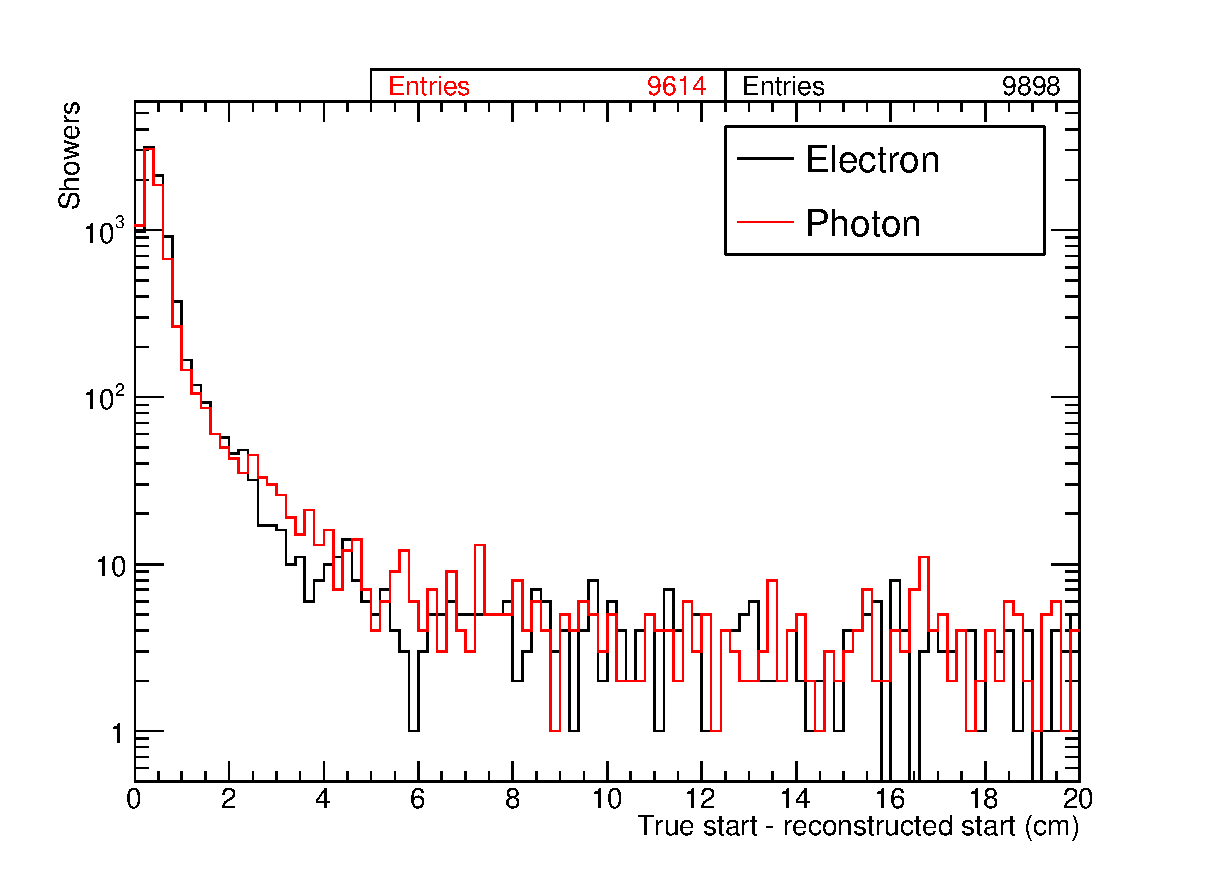
\includegraphics[width=0.98\textwidth]{ShowerStart.eps}
    \caption[The difference between the true and reconstructed shower conversion points.]{The difference between the true and reconstructed shower conversion points.}
    \label{fig:ShowerStart}
  \end{minipage}
  \hfill
  \begin{minipage}[t]{0.48\linewidth}
    \centering
    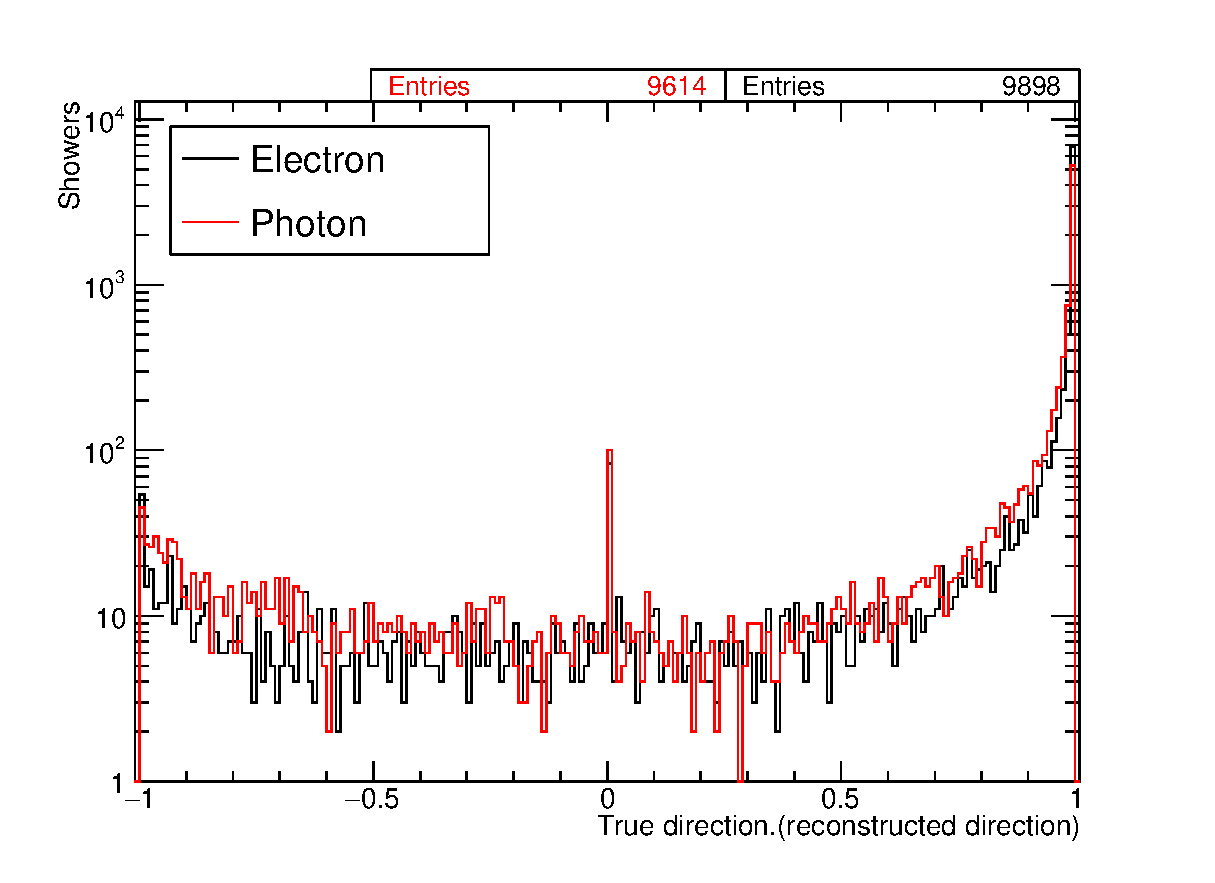
\includegraphics[width=0.98\textwidth]{ShowerDirection.eps}
    \caption[The vector dot product between the true and reconstructed initial shower direction.]{The vector dot product between the true and reconstructed initial shower direction.}
    \label{fig:ShowerDirection}
  \end{minipage}
\end{figure}

The calorimetric information provided by the reconstruction, namely the shower energy and the dE/dx from the initial shower track, is evaluated in Figure~\ref{fig:ShowerEnergy} and~\ref{fig:ShowerdEdx} respectively.  As with the previous validation plots, the reconstruction is shown to produce high quality shower objects.  The energy completeness peaks at around 80\% for both particle species demonstrating a good reconstruction efficiency and good energy conversion.  The reasons for the slightly low peak are due to small issues with fragmentation in the pattern recognition stage, especially towards the lower energy end of a shower, with more sparsely distributed hits, and misunderstandings in the shower energy conversion (described in Section~\ref{sec:ShowerEnergy}).  The dE/dx ionisation information shows very nice separation between electrons and photons, as expected, with the peaks occurring at the anticipated values.

\begin{figure}
  \begin{minipage}[t]{0.48\linewidth}
    \centering
    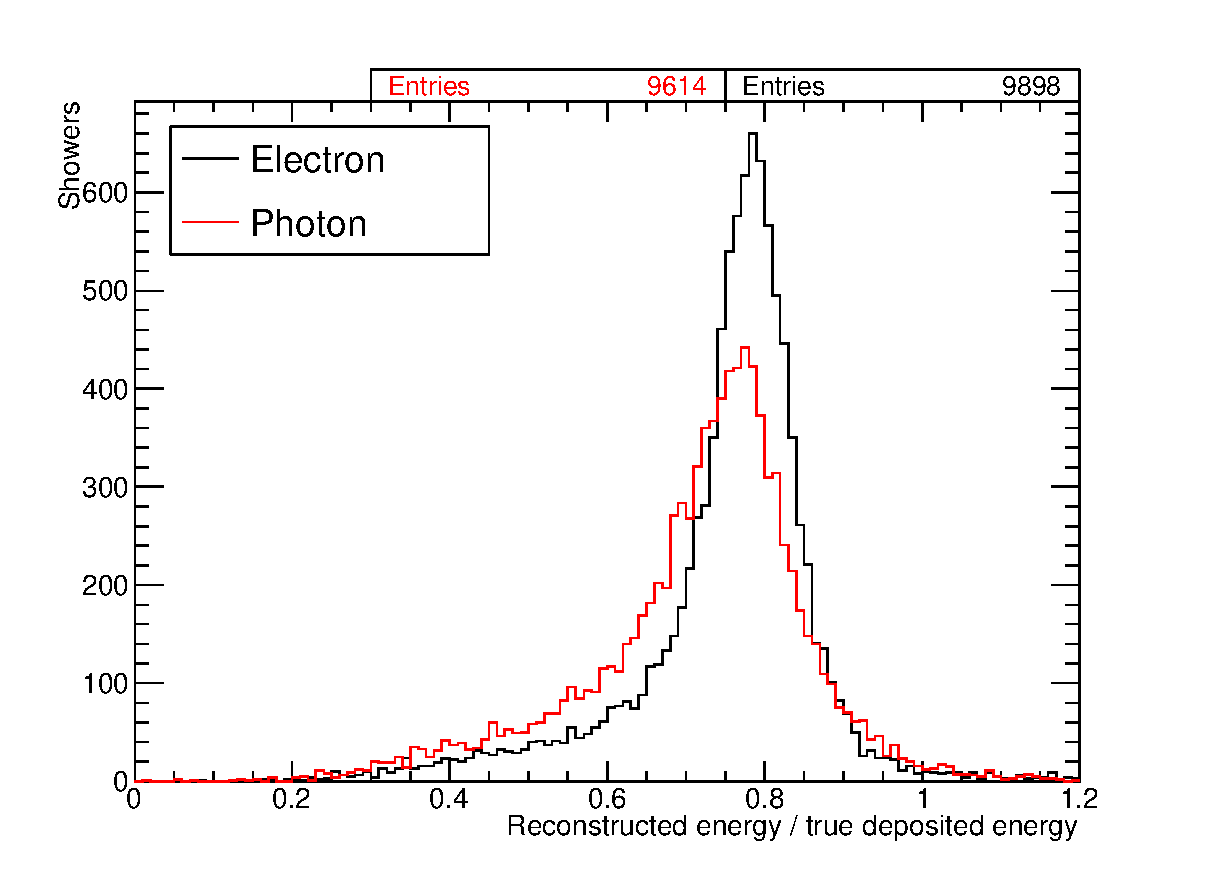
\includegraphics[width=0.98\textwidth]{ShowerDepositedEnergy.eps}
    \caption[The completeness of the reconstruction shower energy when compared with the true deposited energy from simulation.]{The completeness of the reconstruction shower energy when compared with the true deposited energy from simulation.}
    \label{fig:ShowerEnergy}
  \end{minipage}
  \hfill
  \begin{minipage}[t]{0.48\linewidth}
    \centering
    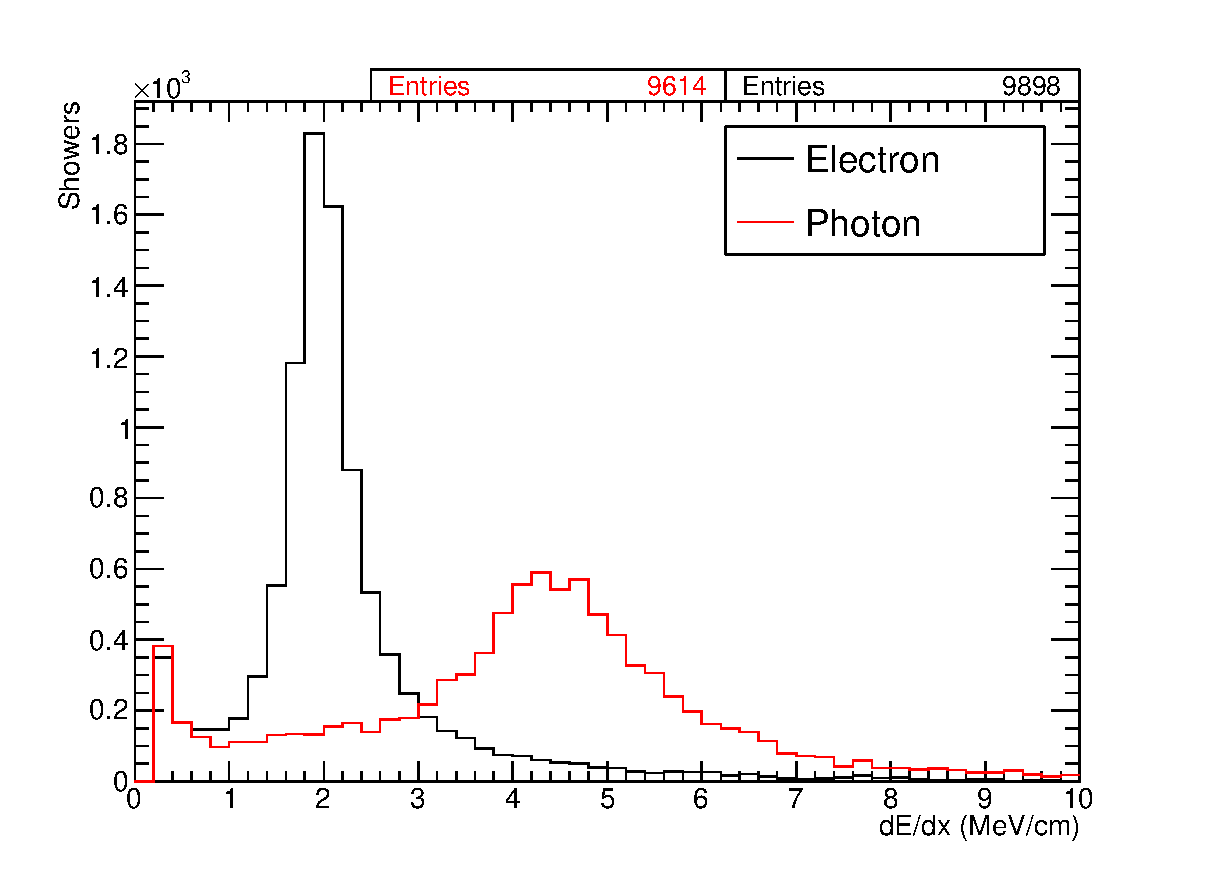
\includegraphics[width=0.98\textwidth]{ShowerdEdx.eps}
    \caption[The dE/dx information from the start of the reconstructed shower object.]{The dE/dx information from the start of the reconstructed shower object.}
    \label{fig:ShowerdEdx}
  \end{minipage}
\end{figure}

%----------------------------------------------------------------------------------------------------------------------------------------------------------------------------
\subsubsection{$\pi^0$ Reconstruction}\label{sec:pi0Reconstruction}

As the primarily motivations for developing the shower reconstruction were to demonstrate successful $\pi^0$ reconstruction, it is instructive to consider the invariant $\pi^0$ mass peak.  This is determined from the two decay photons using
\begin{equation}
  m_{\pi^0} = \sqrt{4 E_{\gamma 1} E_{\gamma 2} \sin^2{\left( \frac{\Delta \theta_{\gamma 1,2}}{2} \right)}},
\end{equation}
where $E_{\gamma n}$ is the energy of each photon and $\Delta \theta_{\gamma 1,2}$ is the angle between the two photon trajectories.

The invariant mass is determined for all $\pi^0$s where both decay photons are considered well reconstructed (i.e. populate the plot shown in Figure~\ref{fig:ShowerReconstructedEnergy}) and the distribution is shown in Figure~\ref{fig:Pi0MassPeak}.  The reconstructed $\pi^0$ mass appears very reasonable when compared to the true value of 135~MeV.  This is a particular challenging reconstruction problem and, when developed via BlurredCluster/EMShower, became the first time it had been solved in LArSoft.

\begin{figure}
  \centering
  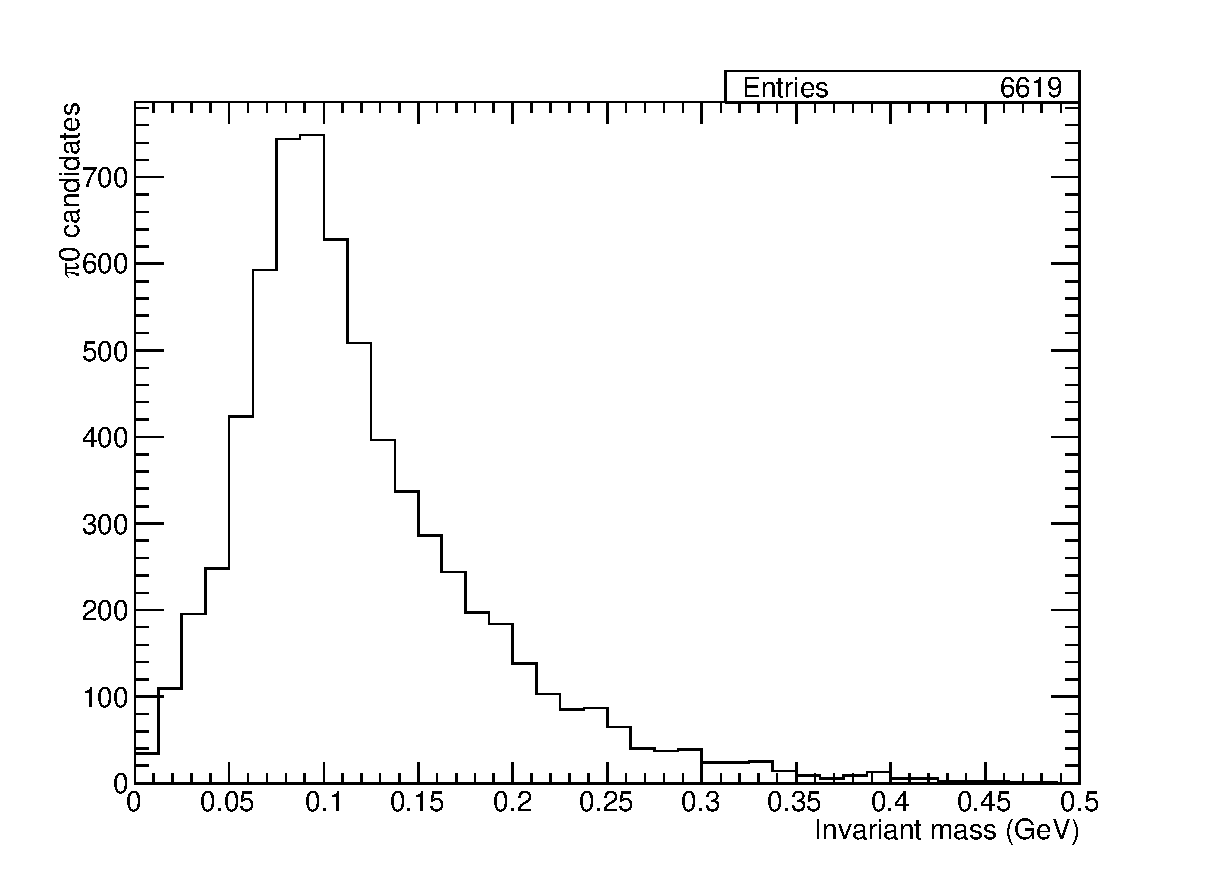
\includegraphics[width=12cm]{Pi0MassPeak.eps}
  \caption[The 35~ton fully reconstructed $\pi^0$ invariant mass peak.]{The 35~ton fully reconstructed $\pi^0$ invariant mass peak.}
  \label{fig:Pi0MassPeak}
\end{figure}

The fully reconstructed $\pi^0$ mass peak differs from expectation in two principal ways: it peaks slightly too low and is relatively broad.  Further analysis is possible by substituting reconstructed quantities for the equivalent true values in the determination of the $\pi^0$ mass.  This is demonstrated in Figure~\ref{fig:Pi0MassPeakTruth}, where the photon energy and direction are successively replaced by their associated true properties.  It may be observed the energy reconstruction causes the peak at a lower mass and the direction reconstruction is responsible for the wide distribution.  This is entirely consistent with observations from the shower reconstruction discussed in Section~\ref{sec:ShowerProperties}.

\begin{figure}
  \centering
  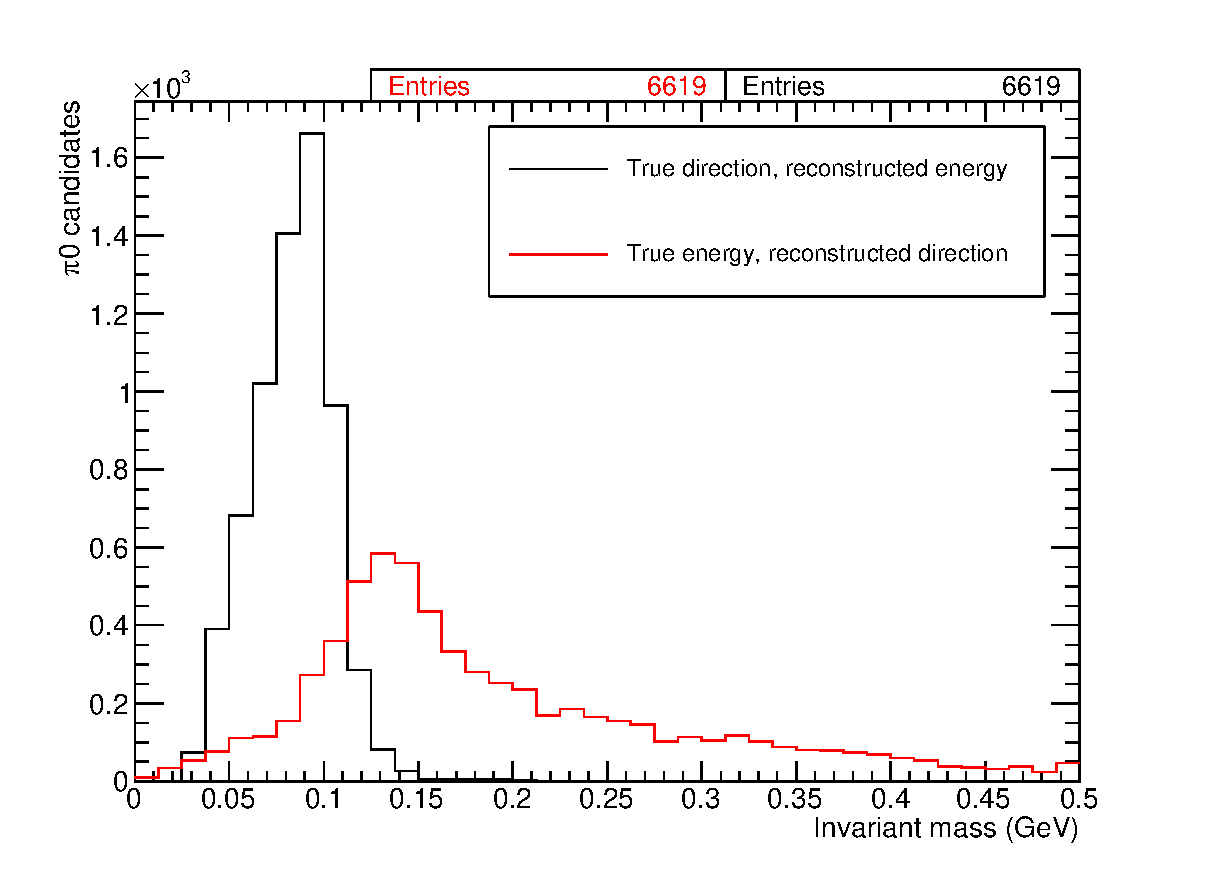
\includegraphics[width=12cm]{Pi0MassPeakTruth.eps}
  \caption[The 35~ton $\pi^0$ mass peak considered using a combination of reconstructed and truth information.]{The 35~ton $\pi^0$ mass peak considered using a combination of reconstructed and truth information.}
  \label{fig:Pi0MassPeakTruth}
\end{figure}

%----------------------------------------------------------------------------------------------------------------------------------------------------------------------------
\subsubsection{Track/Shower Separation Performance}\label{sec:TrackShowerPerformance}

The simple track/shower separation algorithm discussed in Section~\ref{sec:TrackShowerSeparation} is assessed in this present section.  In order to quantify the performance of the reconstruction, the following metrics are defined:
\begin{itemize}
  \item \textit{basic track/shower separation}: the electron shower must be reconstructed as a shower, the longest hadron track originating from the vertex must be identified as a track;
  \item \textit{good shower}: the reconstructed shower start point must be within 10~cm of the true start, the reconstructed direction with $10^{\circ}$ and the shower must be at least 50\% complete;
  \item \textit{good reconstruction}: the event must have basic track/shower separation and the electron shower must be quantified as `good'.
\end{itemize}
Without strictly requiring perfect reconstruction, these metrics have been shown to represent the status of the software reasonably well.  The validation utilised 50~000 DUNE $\nu_e$CC interactions in a reduced far detector volume, intended to represent as closely as possible the oscillation appearance signal.

The efficacy of separating the electron shower from the main hadronic tracks from the vertex, and the reconstruction performance of the electron shower, is demonstrated in Figure~\ref{fig:GoodReconstructionComponents}.  It is clear the challenge is being able to produce well separated particle objects whilst maintaining the shower qualities.  In general the reconstruction performs acceptably but is far from the final solution to this problem.

\begin{figure}
  \centering
  \begin{subfigure}[t]{0.48\linewidth}
    \centering
    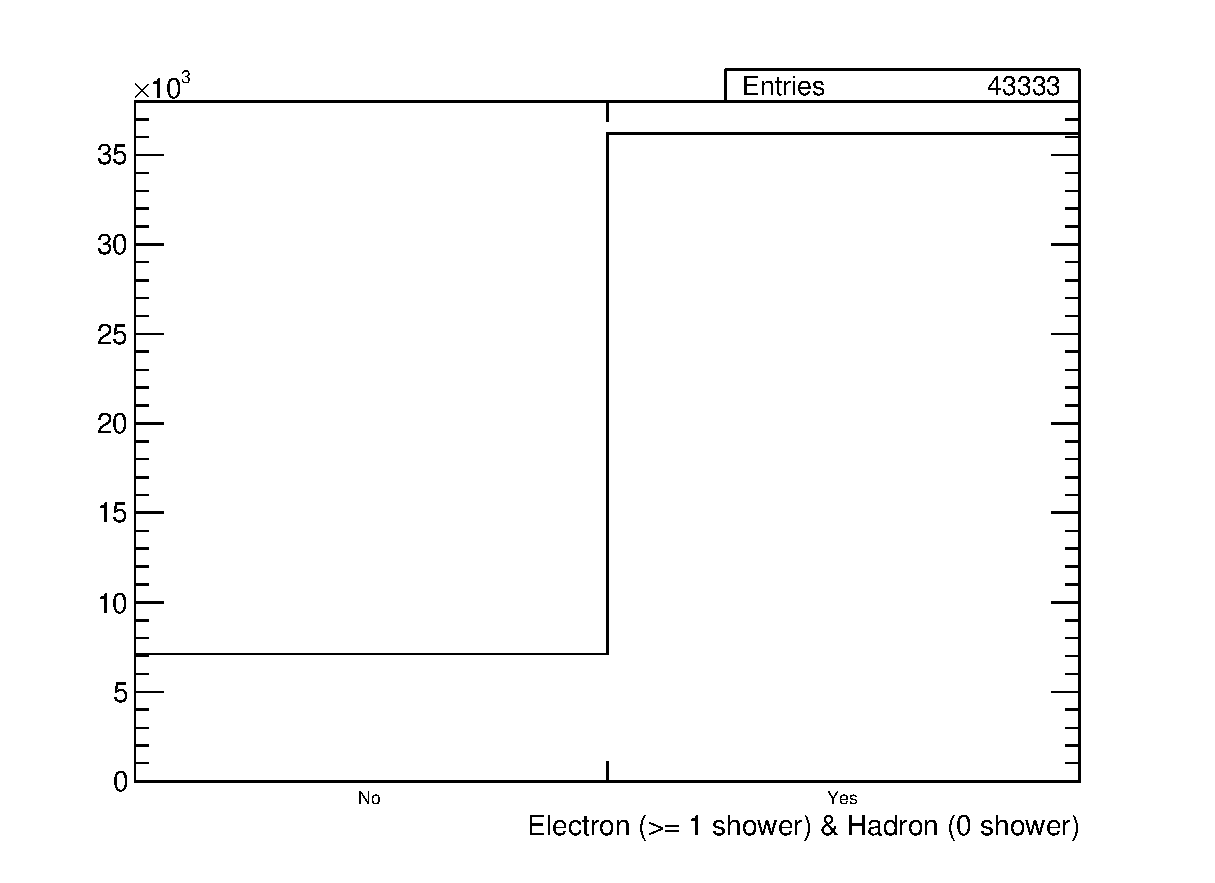
\includegraphics[width=0.98\textwidth]{TrackShowerSeparation.eps}
    \caption{Basic track/shower separation.}
    \label{fig:TrackShowerSeparation}
  \end{subfigure}
  \hfill
  \begin{subfigure}[t]{0.48\linewidth}
    \centering
    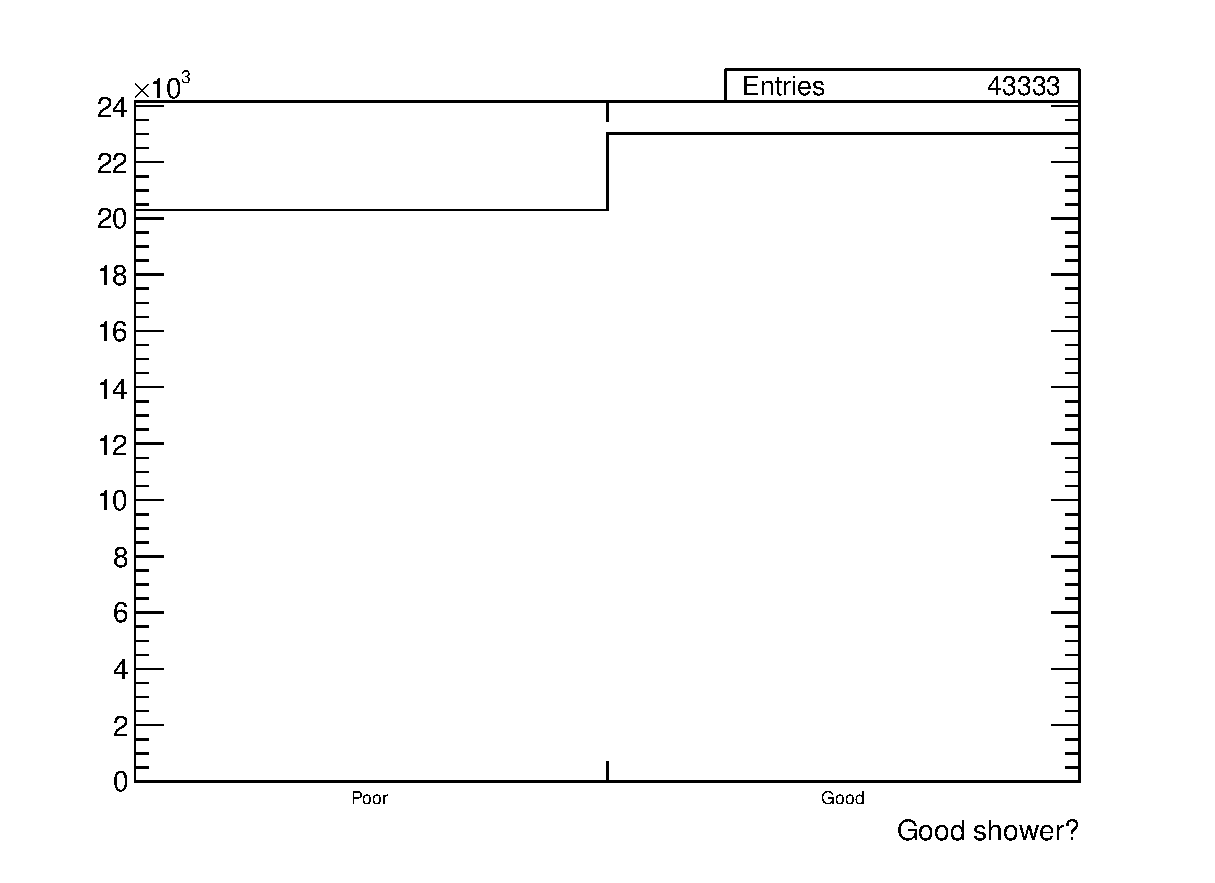
\includegraphics[width=0.98\textwidth]{ElectronGoodShower.eps}
    \caption{Good shower.}
    \label{fig:GoodShower}
  \end{subfigure}
  \caption[Performance of the track/shower separation reconstruction by considering how well separated tracks and showers from the neutrino interaction vertex are and the quality of the reconstructed electron shower.]{Performance of the track/shower separation reconstruction by considering how well separated tracks and showers from the neutrino interaction vertex are and the quality of the reconstructed electron shower.}
  \label{fig:GoodReconstructionComponents}
\end{figure}

The fraction of events which were well reconstructed, considered as a rate and as a function of true neutrino energy, is demonstrated in Figure~\ref{fig:GoodReconstruction}.  The reconstruction performs consistently except at the very lowest energies, when shower completeness becomes the main issue, but only at around 50\% efficiency.  This performance was comparable to, and even slightly superseded, other solutions within LArSoft when developed, but still requires significant improvements.  Much effort has been made recently within the LArSoft collaboration to address this issue directly and good progress has been made.  The experience here has been instructive in how to approach the topic but has demonstrated the successful solution will be attained using a different approach.

\begin{figure}
  \centering
  \begin{subfigure}[t]{0.48\linewidth}
    \centering
    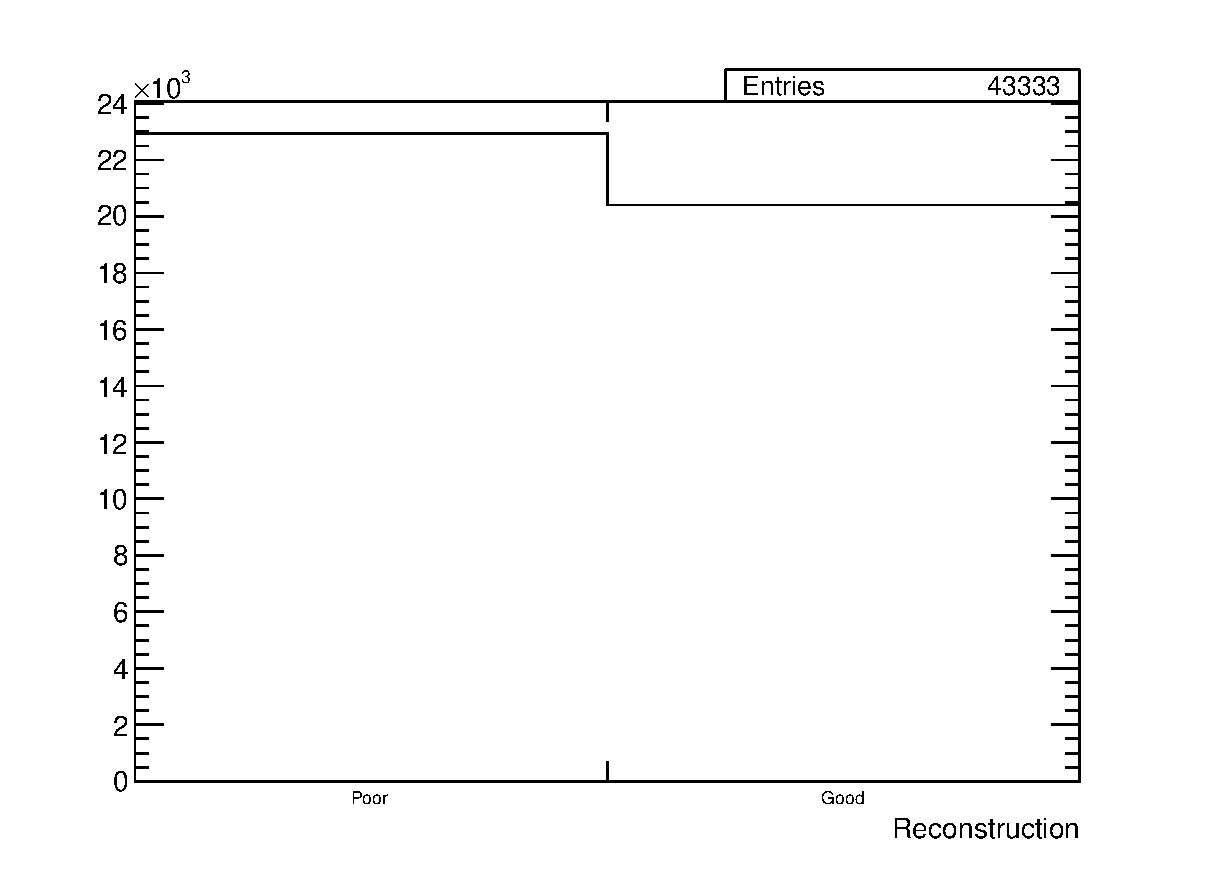
\includegraphics[width=0.98\textwidth]{GoodRecon.eps}
    \caption{Fraction of events with good reconstruction.}
    \label{fig:GoodReconstruction}
  \end{subfigure}
  \hfill
  \begin{subfigure}[t]{0.48\linewidth}
    \centering
    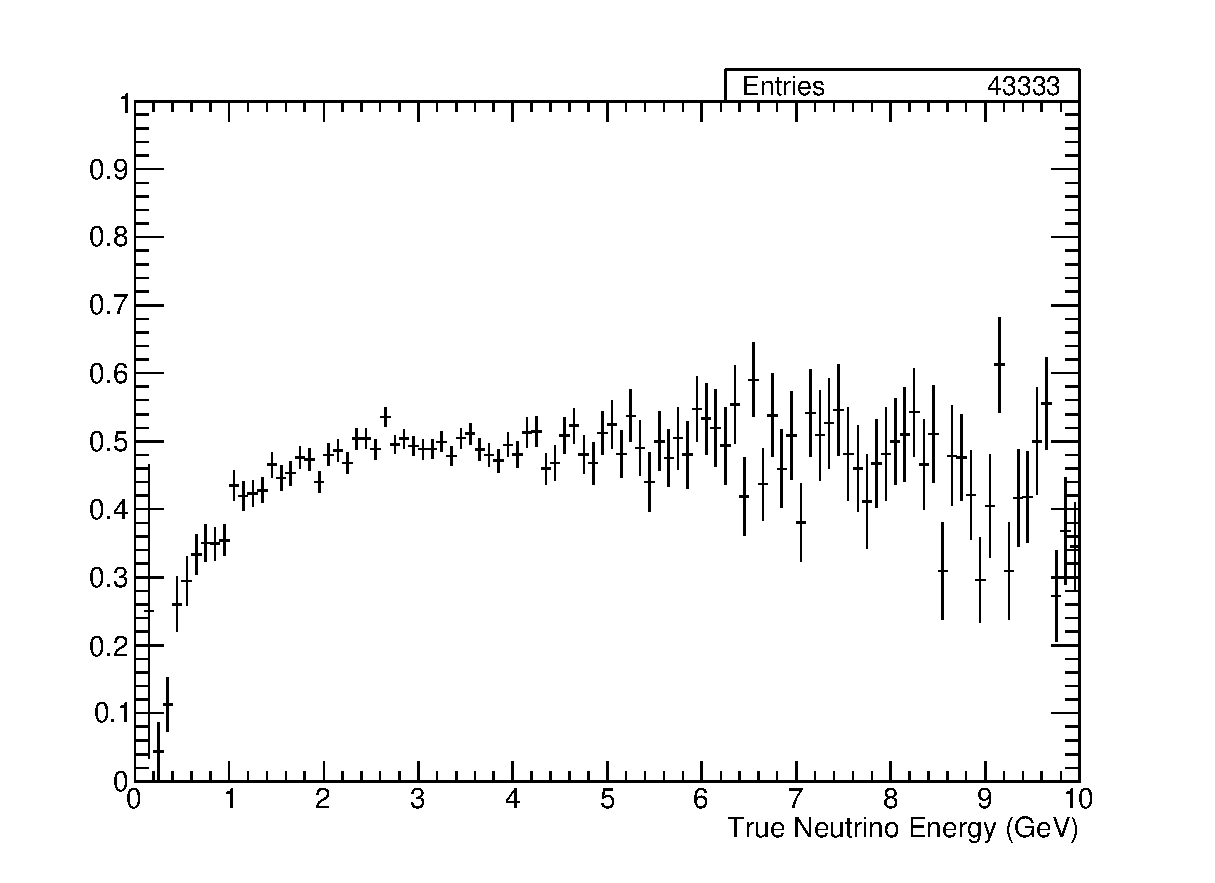
\includegraphics[width=0.98\textwidth]{GoodReconEnergy.eps}
    \caption{The performance of the reconstruction as a function of true neutrino energy.}
    \label{fig:GoodReconstructionEnergy}
  \end{subfigure}
  \caption[The performance of the track/shower separation and shower reconstruction when applied to DUNE $\nu_e$CC far detector interactions.]{The performance of the track/shower separation and shower reconstruction when applied to DUNE $\nu_e$CC far detector interactions.  The performance metrics are defined in the text.}
  \label{fig:GoodReconstruction}
\end{figure}
